% !TeX encoding = UTF-8
% !TeX program = pdflatex
% Maestro final del TFM. Antes del depósito, incorporar aquí la portada oficial,
% el nombre del máster, la institución y la dirección académica.
\documentclass[12pt,a4paper,twoside,openany]{book}

% -----------------------------------------------------------------------------
% Codificación, idioma y tipografía
% -----------------------------------------------------------------------------
\usepackage[utf8]{inputenc}
\usepackage[T1]{fontenc}
\usepackage[spanish,es-nodecimaldot]{babel}
\usepackage{lmodern}
\usepackage{microtype}
\usepackage{csquotes}
\usepackage{xspace}

% -----------------------------------------------------------------------------
% Página y composición
% -----------------------------------------------------------------------------
\usepackage[a4paper,inner=2.5cm,outer=2.5cm,top=3cm,bottom=3cm,
            headheight=28pt]{geometry}
\usepackage{setspace}
\onehalfspacing
\setlength{\parindent}{0.65cm}
\setlength{\parskip}{0pt}
\widowpenalty=10000
\clubpenalty=10000
\displaywidowpenalty=10000
\emergencystretch=2em
\usepackage{fancyhdr}
\usepackage{emptypage}
\pagestyle{fancy}
\fancyhf{}
\fancyhead[LE]{\small\thepage\quad\textsc{Resolución numérica de llamas}}
\fancyhead[RO]{\small\textsc{\leftmark}\quad\thepage}
\renewcommand{\headrulewidth}{0.4pt}
\fancypagestyle{plain}{%
  \fancyhf{}
  \fancyfoot[C]{\thepage}
  \renewcommand{\headrulewidth}{0pt}}

% -----------------------------------------------------------------------------
% Matemática, unidades, tablas y gráficos
% -----------------------------------------------------------------------------
\usepackage{amsmath,amssymb,mathtools,bm}
\usepackage{siunitx}
\sisetup{output-decimal-marker={,},per-mode=symbol,detect-all=true}
\DeclareSIUnit\atmosphere{atm}
\usepackage{booktabs,array,longtable,tabularx,multirow}
\newcolumntype{Y}{>{\raggedright\arraybackslash}X}
\newcolumntype{C}{>{\centering\arraybackslash}X}
\usepackage{graphicx}
\graphicspath{{./}{figuras/}{../}}
\usepackage{float}
\usepackage[section]{placeins}
\usepackage[font=small,labelfont=bf]{caption}
\usepackage{subcaption}
\usepackage{xcolor}
\definecolor{azulTFM}{HTML}{155C8A}
\definecolor{azulElectrico}{HTML}{0066FF}
\definecolor{verdeTFM}{HTML}{2D7F5E}
\definecolor{naranjaTFM}{HTML}{D97706}
\usepackage{tikz}
\usetikzlibrary{arrows.meta,positioning,shapes.geometric,fit,calc,babel}
\usepackage{pgfplots}
\pgfplotsset{compat=1.18}
\usepackage{pgfplotstable}

% -----------------------------------------------------------------------------
% Listas y enlaces
% -----------------------------------------------------------------------------
\usepackage{enumitem}
\setlist{itemsep=0.25em,topsep=0.35em}
\usepackage[unicode]{hyperref}
\hypersetup{
  colorlinks=true,
  linkcolor=blue,
  citecolor=blue,
  urlcolor=blue,
  filecolor=blue,
  pdftitle={Resolución numérica de llamas premezcladas en régimen laminar},
  pdfauthor={Kevin Vidal},
  pdfsubject={Llamas premezcladas laminares, métodos numéricos, solver unidimensional y FGM},
  pdfkeywords={FGM, flamelet, Cantera, PTC-SER, Newton, HPC, combustión}
}
\usepackage[spanish,nameinlink,noabbrev,capitalise]{cleveref}
\crefname{chapter}{Chapter}{Chapters}
\Crefname{chapter}{Chapter}{Chapters}
\crefname{section}{Section}{Sections}
\Crefname{section}{Section}{Sections}
\crefname{figure}{Fig.}{Figs.}
\Crefname{figure}{Fig.}{Figs.}
\crefname{table}{Table}{Tables}
\Crefname{table}{Table}{Tables}
\crefname{equation}{Eq.}{Eqs.}
\Crefname{equation}{Eq.}{Eqs.}

% -----------------------------------------------------------------------------
% Macros y convenciones
% -----------------------------------------------------------------------------
\newcommand{\vect}[1]{\bm{#1}}
\newcommand{\mat}[1]{\bm{#1}}
\newcommand{\dd}{\mathop{}\!\mathrm{d}}
\newcommand{\pd}[2]{\frac{\partial #1}{\partial #2}}
\newcommand{\norm}[1]{\left\lVert #1\right\rVert}
\newcommand{\abs}[1]{\left\lvert #1\right\rvert}
\newcommand{\Su}{S_{\mathrm{u}}}
\newcommand{\Tin}{T_{\mathrm{in}}}
\newcommand{\Tad}{T_{\mathrm{ad}}}
\newcommand{\Yk}{Y_k}
\newcommand{\omegak}{\dot{\omega}_k}
\newcommand{\FGM}{\textsc{FGM}\xspace}
\newcommand{\Vdos}{\textsc{V2}\xspace}
\newcommand{\Cantera}{\textsc{Cantera}\xspace}
\newcommand{\codigo}[1]{\texttt{#1}}


\begin{document}
\hypersetup{pageanchor=false}

% =============================================================================
% Portada y materia preliminar
% =============================================================================
\begin{titlepage}
  \centering
  \vspace*{1.8cm}
  \rule{0.88\textwidth}{0.6pt}\par
  \vspace{0.65cm}
  {\LARGE\bfseries Resolución numérica de llamas premezcladas en régimen laminar\par}
  \vspace{0.45cm}
  {\Large Desarrollo y optimización de un solver unidimensional con aplicación a la generación acelerada de manifolds FGM\par}
  \vspace{0.65cm}
  \rule{0.88\textwidth}{0.6pt}\par
  \vfill
  {\large Trabajo de Fin de Máster\par}
  \vfill
  {\large\textbf{Autor:} Kevin Vidal\par}
  \vfill
  {\large 2026\par}
\end{titlepage}

\cleardoublepage
\pagenumbering{roman}
\hypersetup{pageanchor=true}
\chapter*{Resumen}
\addcontentsline{toc}{chapter}{Resumen}
La resolución de llamas premezcladas laminares libres exige determinar de forma
acoplada la velocidad de propagación, la temperatura y la composición sobre una
malla capaz de resolver una zona reactiva delgada. Este coste se multiplica al
generar familias de flamelets para modelos \emph{flamelet-generated manifold}
(FGM). El presente trabajo desarrolla \Vdos, un solver unidimensional
especializado que combina Newton amortiguado, continuación pseudo-transitoria
PTC--SER, rescate por Euler implícito, adaptación de malla, un Jacobiano
tridiagonal por bloques y un backend nativo para termoquímica, cinética y
transporte.

La metodología se valida principalmente con metano--aire y GRI-Mech~3.0, un
mecanismo detallado de referencia de 53 especies. La comparación con \Cantera
se realiza bajo el mismo mecanismo, modelo de transporte y criterios de
aceptación, y separa la convergencia no lineal, la independencia espacial y la
coherencia física del rendimiento. En el nivel espacial más fino del caso
estequiométrico, \Vdos y \Cantera predijeron velocidades de
\SI{0.376287}{\metre\per\second} y \SI{0.376441}{\metre\per\second},
respectivamente, una diferencia de \SI{0.041}{\percent}. En un barrido frío de
cinco mezclas, el tiempo acumulado fue \SI{28.32}{\second} para \Vdos y
\SI{61.38}{\second} para \Cantera; esta comparación temporal se considera
preliminar hasta completar repeticiones alternadas. La ablación de la región de
confianza mostró, además, que reutilizar una solución fuera de una vecindad
paramétrica local puede aumentar sustancialmente el coste, lo que justifica una
continuación protegida por criterios de aceptación.

Como extensión, se implementó transporte multicomponente con Soret y se evaluó
en hidrógeno--aire. La aplicación FGM construye una tabla en coordenadas
\((Z,c)\) a partir de flamelets previamente certificados. La validación por
exclusión mostró que cinco valores de mezcla son insuficientes para una tabla de
producción, con errores de liberación de calor de hasta \SI{27.9}{\percent}.
Por tanto, la contribución no se formula como una nueva física de llama, sino
como una arquitectura reproducible orientada a reducir el tiempo extremo a
extremo necesario para obtener familias de soluciones aceptadas y a identificar
con claridad el dominio en el que esa especialización resulta ventajosa.

\textbf{Palabras clave:} combustión premezclada; llamas laminares; FGM;
continuación pseudo-transitoria; Newton; malla adaptativa; Cantera; transporte
multicomponente; Soret.

\cleardoublepage
\chapter*{Abstract}
\addcontentsline{toc}{chapter}{Abstract}
Freely propagating premixed laminar flames require the coupled determination of
flame speed, temperature, and composition on a mesh capable of resolving a thin
reaction zone. This cost is multiplied when families of flamelets are generated
for flamelet-generated manifold (FGM) models. This work develops \Vdos, a
specialised one-dimensional solver that combines damped Newton iterations,
PTC--SER pseudo-transient continuation, a backward-Euler rescue, adaptive
meshing, a tridiagonal por bloques Jacobian, and a native backend for thermochemistry,
kinetics, and transport.

The methodology is validated primarily for methane--air using GRI-Mech~3.0, a
53-species detailed reference mechanism. Comparisons with \Cantera use the same
mechanism, transport model, and acceptance criteria, and distinguish nonlinear
convergence, spatial convergence, and physical consistency from performance. On
the finest spatial level for the stoichiometric case, \Vdos and \Cantera
predicted flame speeds of \SI{0.376287}{\metre\per\second} and
\SI{0.376441}{\metre\per\second}, respectively, a
\SI{0.041}{\percent} difference. In a cold five-mixture sweep, accumulated
solution times were \SI{28.32}{\second} for \Vdos and
\SI{61.38}{\second} for \Cantera; this timing comparison remains
preliminary until alternating repetitions are completed. A trust-region
ablation further showed that reusing a converged solution outside a local
parameter neighbourhood can substantially increase cost, which motivates
acceptance-aware bounded continuation.

As an extension, native multicomponent transport with Soret diffusion was
implemented and evaluated for hydrogen--air. The FGM application constructs a
\((Z,c)\) table from previously certified flamelets. Leave-one-mixture-out
validation showed that five mixture values are insufficient for a production
manifold, with heat-release errors reaching \SI{27.9}{\percent}. The main
contribution is therefore not a new flame model, but a reproducible architecture
for reducing the end-to-end cost of obtaining accepted families of laminar
flames while explicitly delimiting the regime in which the specialised strategy
is advantageous.

\textbf{Keywords:} premixed combustion; laminar flames; FGM; pseudo-transient
continuation; Newton method; adaptive mesh; Cantera; multicomponent transport;
Soret diffusion.

\cleardoublepage
\tableofcontents
\cleardoublepage
\listoffigures
\cleardoublepage
\listoftables

\cleardoublepage
\chapter*{Nomenclatura}
\addcontentsline{toc}{chapter}{Nomenclatura}
\markboth{Nomenclatura}{Nomenclatura}
La tesis emplea unidades SI. Las cantidades molares del backend se expresan por
\(\mathrm{kmol}\); por tanto, \(W_k\) se usa en \(\mathrm{kg\,kmol^{-1}}\).
Un subíndice \(j\) identifica un nodo espacial, \(k\) una especie y \(r\) una
reacción. Los símbolos se reúnen a continuación por familia para evitar
introducir definiciones dispersas en capítulos posteriores.

\begin{longtable}{@{}p{0.25\textwidth}p{0.63\textwidth}@{}}
\toprule
\textbf{Símbolo latino} & \textbf{Definición} \\
\midrule
\endhead
\(A_r,b_r,E_{a,r}\) & Factor preexponencial, exponente térmico y energía de activación de la reacción \(r\). \\
\(a_{i,k}\) & Coeficiente \(i\) del polinomio termoquímico NASA de la especie \(k\). \\
\(\mat A_j,\mat B_j,\mat C_j,\mat L_j\) & Bloques inferior, diagonal, superior y multiplicador de la eliminación lineal. \\
\(\mat P_j,\mat L_j^{\rm LU},\mat U_j\) & Matriz de permutación y factores triangular inferior y superior del bloque pivotado. \\
\(\mathcal A,\mathcal A_\ell\) & Predicado global de aceptación y condición de su capa \(\ell\). \\
\(c\) & Variable de progreso normalizada del manifold. \\
\(c_p,c_{p,k}\) & Capacidades caloríficas específicas de mezcla y especie a presión constante. \\
\(C_k\) & Concentración molar de la especie \(k\). \\
\(D_k\) & Coeficiente de difusión promediado por mezcla de la especie \(k\). \\
\(D_z,D\) & Operadores discretos de derivación espacial. \\
\(d,d_{\rm tr}\) & Dimensión del vector de control del manifold y distancia de confianza paramétrica. \\
\(\mathrm{Da},\mathrm{Le}_k,\mathrm{Ma}\) & Números de Damköhler, Lewis y Mach. \\
\(E_2,\Delta_{\infty},E_m,E_Y\) & Error relativo de perfil, diferencia máxima absoluta, error de flujo másico y cierre de composición. \\
\(e_J,e_q\) & Errores de verificación direccional del Jacobiano y de validación cruzada de tabla. \\
\(\vect e_i\) & Vector canónico asociado a la variable global \(i\). \\
\(\vect F,\mat J_F\) & Residual estacionario discreto y su Jacobiano. \\
\(F_{\rm guard}\) & Límite independiente del residual usado para aceptar convergencia no lineal. \\
\(\vect G,\mat J_G\) & Residual de Euler implícito y su Jacobiano. \\
\(g(c),G(c)\) & Indicador FGM de actividad y su distribución acumulada normalizada. \\
\(h,h_k^{\mathrm{mol}},h_k^{\mathrm{mass}}\) & Entalpía de mezcla y entalpías molar y másica de la especie \(k\). \\
\(h_j^-,h_j^+,h_j^c\) & Distancias izquierda, derecha y total del stencil del nodo \(j\). \\
\(J_k,J_k^*\) & Flujo difusivo másico corregido y flujo preliminar de la especie \(k\). \\
\(j_a,T_a\) & Índice y temperatura prescrita del nodo de anclaje. \\
\(k_{f,r},k_{b,r},q_r\) & Constantes directa e inversa y tasa de progreso de la reacción \(r\). \\
\(K,N,n_v\) & Número de especies, nodos y variables por nodo. \\
\(L\) & Longitud del dominio unidimensional. \\
\(\mat M\) & Matriz de masa diagonal del sistema pseudo-transitorio. \\
\(\mathcal M,\vect q\) & Aplicación del manifold y vector de estado termoquímico reconstruido. \\
\(\mathcal I,\mathcal Q,\mathcal S\) & Operador de interpolación y conjuntos de campos y especies seleccionados. \\
\(\dot m,m_j,\overline{\dot m}\) & Flujo másico por unidad de área, valor nodal \(\rho_j u_j\) y promedio nodal. \\
\(n_j,N_{\rm tabla}\) & Nodos del eje \(j\) y número total de estados de una tabla. \\
\(p,p_0\) & Presión termodinámica y su valor uniforme de bajo Mach. \\
\(q_c,\dot q\) & Flujo conductivo y liberación volumétrica de calor. \\
\(q_{\rm abs},s_q\) & Escalas de regularización absoluta y normalización de un campo \(q\). \\
\(R\) & Constante universal de los gases. \\
\(\vect r_{\rm lin}\) & Defecto a posteriori entre el residual no lineal y su predicción lineal. \\
\(r_\phi,r_h\) & Radios de confianza en equivalencia y defecto de entalpía. \\
\(R_j,S_{\psi,j},C_{\psi,j},P\) & Indicadores de ratio, pendiente y curvatura de malla, y umbral de poda. \\
\(R_{\max},S_{\max},C_{\max}\) & Umbrales de inserción de los tres indicadores de malla. \\
\(\vect s,w_v\) & Corrección no lineal y escala ponderada de la variable física \(v\). \\
\(S_t,S_{t,5\phi}\) & Aceleración temporal de una llama y del barrido de cinco mezclas. \\
\(\Su\) & Velocidad de llama laminar referida a la mezcla no quemada. \\
\(t_{\rm solve}\) & Tiempo exclusivo de resolución de una llama. \\
\(T,\Tin,\Tad,T_{\mathrm u},T_{\mathrm b}\) & Temperatura local, de entrada, adiabática, no quemada y quemada. \\
\(u,V_k\) & Velocidad axial y velocidad difusiva de la especie \(k\). \\
\(W,W_k\) & Masa molar de mezcla y de la especie \(k\). \\
\(w_T,w_q,w_k\) & Pesos del indicador adaptativo de progreso. \\
\(X_k,Y_k\) & Fracciones molar y másica de la especie \(k\). \\
\(\vect x,\vect x^{\rm tr},\vect x^n\) & Estado discreto, estado candidato y estado del nivel pseudo-temporal anterior. \\
\(z,Z\) & Coordenada espacial y fracción de mezcla de Bilger. \\
\(Z_e\) & Fracción másica del elemento químico \(e\). \\
\bottomrule
\end{longtable}

\begin{longtable}{@{}p{0.25\textwidth}p{0.63\textwidth}@{}}
\toprule
\textbf{Símbolo griego} & \textbf{Definición} \\
\midrule
\endhead
\(\alpha_T\) & Difusividad térmica de mezcla, \(\lambda/(\rho c_p)\). \\
\(\alpha_\ell\) & Factor de amortiguamiento de la iteración no lineal \(\ell\). \\
\(\beta_{\mathrm B},\beta_c\) & Escalar elemental de Bilger y progreso químico no normalizado. \\
\(\gamma,\gamma_t\) & Amortiguamiento de los predictores secante y tangente.
\\
\(\ell\) & Coordenada de continuación, \(\ell=\log\phi\). \\
\(\delta,\delta_T\) & Escala espacial genérica y espesor térmico de llama. \\
\(\delta_{\mathrm{abs}},\delta_{\mathrm{rel}}\) & Perturbaciones absoluta y relativa del Jacobiano por diferencias finitas. \\
\(\delta_i\) & Perturbación total aplicada a la columna \(i\) del Jacobiano. \\
\(\delta_{\rm lin,j},\epsilon_{\rm lin}\) & Indicador local de defecto de linealización y su escala de regularización. \\
\(\Delta h,\Delta\tau,\Delta\psi\) & Defecto de entalpía, paso pseudo-temporal y rango de un perfil de malla. \\
\(\Delta z_j^-,\Delta z_j^+,\Delta z_j^c\) & Espaciados izquierdo, derecho y total del stencil principal. \\
\(\boldsymbol\eta,\eta_k\) & Vector de control del manifold y peso de concentración de una especie en el indicador FGM. \\
\(\eta_i\) & Indicador de error para insertar un nuevo flamelet paramétrico. \\
\(\varepsilon_{\Su},\delta_q^{(r)}\) & Diferencia relativa de velocidad de llama y cambio entre ciclos de malla. \\
\(\varepsilon_a,\varepsilon_r\) & Tolerancias absoluta y relativa usadas en la norma ponderada. \\
\(\epsilon,\varepsilon_\psi,\varepsilon_d\) & Regularizadores positivos para la malla FGM y los indicadores espaciales. \\
\(\lambda\) & Conductividad térmica. \\
\(\mu_i\) & Entrada diagonal de la matriz de masa: uno para fila diferencial y cero para fila algebraica. \\
\(\nu'_{kr},\nu''_{kr}\) & Coeficientes estequiométricos de reactivos y productos. \\
\(\rho\) & Densidad de la mezcla. \\
\(\phi\) & Relación de equivalencia combustible--oxidante. \\
\(\tau_{\mathrm{tr}},\tau_{\mathrm q}\) & Escalas temporales de transporte y química. \\
\(\dot\omega_k^{\mathrm{mol}},\dot\omega_k^{\mathrm{mass}}\) & Tasas netas de producción molar y másica. \\
\(\dot\omega_c\) & Fuente másica normalizada de la variable de progreso tabulada. \\
\(\psi\) & Variable escalar genérica usada en derivadas e indicadores de malla. \\
\bottomrule
\end{longtable}

\begin{longtable}{@{}p{0.25\textwidth}p{0.63\textwidth}@{}}
\toprule
\textbf{Índice} & \textbf{Significado} \\
\midrule
\endhead
\(\mathrm{ad},\mathrm b,\mathrm{in},\mathrm u\) & Adiabático, quemado, entrada y no quemado. \\
\(a,\mathrm{exc}\) & Nodo de anclaje y especie de exceso usada para normalización. \\
\(\mathrm f,\mathrm{ox}\) & Corrientes de combustible y oxidante. \\
\(j,j\!+\!1/2\) & Nodo y cara entre los nodos \(j\) y \(j+1\). \\
\(k,r\) & Índices de especie y reacción. \\
\(\mathrm{mol},\mathrm{mass}\) & Bases molar y másica. \\
\((\cdot)^*,\overline{(\cdot)}\) & Valor preliminar y promedio entre caras. \\
\(m,n,\mathrm{tr}\) & Iteración de Newton, nivel pseudo-temporal y estado de prueba. \\
\bottomrule
\end{longtable}

\begin{longtable}{@{}p{0.25\textwidth}p{0.63\textwidth}@{}}
\toprule
\textbf{Sigla} & \textbf{Significado} \\
\midrule
\endhead
BE & Euler implícito (\emph{backward Euler}). \\
BLAS/LAPACK & Bibliotecas básicas de álgebra lineal y de álgebra lineal numérica. \\
CFD & Dinámica de fluidos computacional (\emph{computational fluid dynamics}). \\
CPU & Unidad central de procesamiento. \\
CSV & Archivo de valores separados por comas. \\
FD & Diferencias finitas (\emph{finite differences}). \\
FGM & Manifold generado por flamelets (\emph{flamelet-generated manifold}). \\
FPI/FPV & Prolongación flamelet de ILDM y modelo flamelet/variable de progreso. \\
GRI-Mech & Mecanismo cinético detallado para combustión de gas natural. \\
HP & Equilibrio a entalpía y presión constantes. \\
HPC & Computación de alto rendimiento. \\
ILDM & Manifold intrínseco de baja dimensión. \\
ISAT & Tabulación adaptativa en ejecución (\emph{in-situ adaptive tabulation}). \\
JIT & Compilación en tiempo de ejecución (\emph{just in time}). \\
JSON/NPZ & Formatos de metadatos y arreglos comprimidos empleados en las salidas. \\
LES/RANS & Simulación de grandes escalas y ecuaciones de Reynolds promediadas. \\
LLVM & Infraestructura de compilación empleada indirectamente por Numba. \\
LU & Factorización triangular inferior--superior. \\
NASA & Administración Nacional de Aeronáutica y el Espacio; designa aquí sus polinomios termoquímicos. \\
NOx & Óxidos de nitrógeno. \\
PDF & Función de densidad de probabilidad en el contexto de modelado de combustión. \\
PREMIX & Solver unidimensional histórico para llamas premezcladas. \\
PTC & Continuación pseudo-transitoria. \\
SER & Relajación de evolución conmutada (\emph{switched evolution relaxation}). \\
SI & Sistema Internacional de Unidades. \\
TFM & Trabajo Fin de Máster. \\
\Vdos & Solver especializado desarrollado en este trabajo. \\
\bottomrule
\end{longtable}

\begin{longtable}{@{}p{0.25\textwidth}p{0.63\textwidth}@{}}
\toprule
\textbf{Término técnico} & \textbf{Uso en esta tesis} \\
\midrule
\endhead
Backend & Núcleo que evalúa propiedades, cinética o transporte detrás de la interfaz del solver. \\
Caché & Almacenamiento persistente de perfiles certificados para reutilizarlos como semillas. \\
Flamelet & Solución canónica unidimensional que aporta estados al manifold. \\
Kernel & Rutina computacional intensiva, normalmente compilada y repetida sobre muchos nodos. \\
Disposición & Orden de almacenamiento de las variables en memoria. \\
Manifold & Variedad termoquímica de dimensión reducida parametrizada por variables de control. \\
Solver & Conjunto de algoritmos que ensambla y resuelve el problema discreto. \\
Stencil & Conjunto de nodos que intervienen en una aproximación espacial local. \\
\emph{Speedup} & Cociente entre el tiempo de referencia y el tiempo del método evaluado. \\
\emph{Upwind} & Discretización convectiva aguas arriba. \\
\bottomrule
\end{longtable}

\cleardoublepage
\pagenumbering{arabic}

% =============================================================================
\chapter{Introducción}
\label{chap:introduccion}

\section{Motivación y contexto}

La combustión continúa desempeñando un papel relevante en turbinas de gas,
motores, hornos industriales y sistemas energéticos que incorporan combustibles
convencionales o alternativas como hidrógeno y amoníaco. Su simulación es
costosa porque la dinámica del flujo, el transporte molecular y la cinética
química detallada operan sobre escalas muy diferentes y permanecen fuertemente
acopladas \cite{Peters1984,Poinsot2005,Kee2017}. En una simulación
tridimensional, este coste se repite en cada celda y paso temporal, de modo que
la evaluación de especies, tasas de reacción y propiedades puede limitar la
exploración sistemática de diseños y condiciones de operación.

Los métodos de reducción de química buscan conservar la respuesta termoquímica
relevante sin transportar explícitamente todo el espacio de especies. Entre
ellos se encuentran los manifolds intrínsecos de baja dimensión, la tabulación
adaptativa y los enfoques basados en flamelets
\cite{MaasPope1992,Pope1997,Peters1984}. El método FGM construye una
representación de baja dimensión a partir de soluciones canónicas de llama y
permite consultar posteriormente el estado termoquímico mediante pocas
variables de control \cite{vanOijen2000,vanOijenReview2016}.

La reducción, sin embargo, no elimina el coste de la química; desplaza una parte
importante hacia el preprocesamiento. Cada fila del manifold procede de una
llama que debe converger, satisfacer balances y disponer de resolución espacial
suficiente antes de ser tabulada. Cuando se incorporan presión, entalpía,
deformación o transporte preferencial, el número de flamelets aumenta y el
tiempo acumulado de generación puede convertirse en un cuello de botella
\cite{DoniniThesis2014,vanOijenReview2016}. Por ello, en una campaña FGM la
pregunta relevante no es únicamente cuánto cuesta una iteración, sino cuánto
tiempo requiere obtener una familia completa de soluciones aceptadas.

\section{Planteamiento y justificación del problema}

Una llama premezclada laminar libre constituye un problema no lineal de contorno
en el que la velocidad de propagación no se prescribe. En un sistema ligado al
frente, el flujo másico, la temperatura y la composición se determinan de forma
acoplada; además, la invariancia por traslación exige una condición de anclaje
que fije la posición de la llama sin imponer su velocidad. La química detallada
añade rigidez, escalas muy diferentes y una zona reactiva estrecha, por lo que
la solución requiere combinar discretización conservativa, globalización no
lineal, adaptación de malla y controles de dominio.

Esta cadena impone una condición esencial para cualquier comparación de
rendimiento: una ejecución más rápida solo constituye una mejora si alcanza una
solución de calidad comparable. En consecuencia, este TFM adopta como métrica
principal el \emph{tiempo extremo a extremo hasta una llama aceptada}, entendido
como el coste de resolver el sistema no lineal, adaptar la malla y superar los
controles definidos de estado, conservación y suficiencia espacial.

\section{Posicionamiento frente a la literatura}

La resolución de llamas unidimensionales con química detallada cuenta con una
tradición consolidada. PREMIX estableció una arquitectura basada en Newton,
integración transitoria de respaldo y adaptación de malla
\cite{Grcar1988,KeePremix1998}, y herramientas actuales como \Cantera,
FlameMaster u OpenSMOKE++ mantienen formulaciones robustas de propósito general.
Las comparaciones entre marcos muestran que, cuando se igualan las hipótesis
físicas y la resolución espacial, las predicciones de llamas premezcladas pueden
alcanzar una concordancia elevada \cite{Langer2018}. Por ello, el presente
trabajo no parte de que los solvers existentes sean inadecuados ni presenta como
novedades aisladas a Newton, PTC, la adaptación de malla o la estructura
matricial local.

La reducción específica del tiempo de solución también ha sido estudiada.
Lapointe et al. desarrollaron métodos dispersos e iterativos para mecanismos que
alcanzan miles de especies \cite{Lapointe2019}, mientras que Perini et al.
combinaron Jacobianos analíticos dispersos, solvers iterativos, paralelización y
refinamiento progresivo \cite{Perini2025}. Estos trabajos muestran que el
beneficio de una estrategia depende del tamaño y de la estructura del problema.
En la misma dirección, Wu et al. observaron que la elección entre álgebra densa
y dispersa cambia al crecer el mecanismo \cite{Wu2023}.

El régimen estudiado aquí es deliberadamente más acotado. Se emplea GRI-Mech~3.0,
un mecanismo detallado de referencia de 53 especies, para aislar y validar la
metodología numérica antes de considerar mecanismos cinéticos grandes. En este
régimen se investiga si explotar la estructura tridiagonal por bloques, reducir
la sobrecarga de evaluaciones repetitivas y reutilizar de forma controlada
soluciones paramétricamente próximas disminuye el coste acumulado de una familia
de llamas. \Cantera se mantiene como referencia independiente; \Vdos se usa
como plataforma de investigación especializada, no como sustituto universal.

\section{Objetivos}

\subsection{Objetivo general}

Desarrollar, optimizar y validar una metodología numérica reproducible para
resolver de forma eficiente familias de llamas premezcladas laminares
unidimensionales, reduciendo el tiempo extremo a extremo respecto de una
referencia \Cantera sin degradar materialmente la fidelidad física y numérica,
y demostrar su aplicación a la generación de tablas FGM.

\subsection{Objetivos específicos}

\begin{enumerate}
  \item Formular las ecuaciones estacionarias de continuidad, especies y
        energía para una llama premezclada libre, con condiciones de contorno y
        transporte coherentes con el modelo adoptado.
  \item Discretizar el problema preservando la localidad espacial para explotar
        la estructura tridiagonal por bloques del Jacobiano.
  \item Implementar una estrategia robusta que combine Newton amortiguado,
        continuación pseudo-transitoria PTC--SER y rescate por Euler implícito.
  \item Verificar estado, conservación, convergencia no lineal, independencia
        espacial y suficiencia del dominio antes de aceptar una llama.
  \item Comparar \Vdos y \Cantera bajo condiciones físicas y criterios de
        aceptación equivalentes, utilizando velocidad de llama, perfiles,
        balances y tiempo de ejecución.
  \item Cuantificar mediante ablaciones el efecto de optimizaciones concretas,
        en particular la sustitución compilada por bloques, la continuación
        paramétrica acotada y el refresco local del Jacobiano.
  \item Extender la metodología a transporte multicomponente con Soret y
        delimitar la evidencia disponible para este régimen.
  \item Construir una cadena FGM común a ambas rutas y verificar mediante
        exclusión de mezclas si la discretización paramétrica es suficiente.
\end{enumerate}

\section{Contribuciones y originalidad}

La contribución se sitúa en la integración y evaluación causal de técnicas
conocidas dentro de un flujo especializado y certificado. En concreto, el
trabajo aporta: (i) una implementación instrumentable de la llama libre 1D;
(ii) una resolución directa que conserva el pivotado de los bloques y fusiona
las sustituciones repetidas en un kernel compilado; (iii) una estrategia
Newton--PTC--BE asociada a criterios explícitos de aceptación; (iv) continuación
paramétrica que reutiliza únicamente soluciones previamente aceptadas dentro de
una vecindad declarada; (v) un refresco local del Jacobiano activado mediante un
defecto de linealización; y (vi) una cadena FGM en la que la calidad del solver
y la suficiencia del muestreo paramétrico se verifican por separado.

La originalidad no se formula, por tanto, como la invención de cada componente,
sino como una arquitectura de \emph{tiempo hasta aceptación} cuya evidencia se
obtiene mediante comparaciones completas y ablaciones, evitando extrapolar un
microbenchmark aislado al rendimiento del solver. Esta delimitación es
coherente con la literatura previa y permite distinguir con precisión qué
resultados han sido demostrados y cuáles permanecen como extensiones futuras.

\section{Alcance y limitaciones}

La campaña principal considera llamas planas, estacionarias y premezcladas a
presión constante, con metano--aire, \SI{300}{\kelvin},
\SI{1}{\atmosphere} y GRI-Mech~3.0. El caso base emplea transporte promediado
por mezcla y no incluye Soret. Como extensión se implementa transporte
multicomponente con termodifusión y se presentan resultados iniciales para
hidrógeno--aire. Radiación, formación de hollín, química superficial y
configuraciones multidimensionales permanecen fuera del alcance.

Los resultados con 53 especies no demuestran escalabilidad hacia mecanismos con
centenares o miles de especies. En ese régimen deberán evaluarse de nuevo el
balance entre factorización directa, álgebra dispersa, métodos de Krylov,
precondicionamiento y paralelización \cite{Lapointe2019,Wu2023,Perini2025}.
Asimismo, los tiempos de una única ejecución se identifican como preliminares y
no sustituyen una campaña estadística. La aplicación FGM se considera validada
como cadena de generación, pero no como tabla lista para CFD mientras la
validación por exclusión indique resolución insuficiente en el eje paramétrico.

\section{Estructura del documento}

El \cref{chap:marco-teorico} presenta los fundamentos físicos y el estado del
arte necesarios para situar el problema y las estrategias numéricas. El
\cref{chap:metodologia} desarrolla el modelo, la discretización, el solver
\Vdos, la extensión de transporte y la metodología FGM, junto con el protocolo
de comparación y reproducibilidad. El \cref{chap:resultados} reúne únicamente
la evidencia obtenida, mientras que el \cref{chap:discusion} interpreta esos
resultados frente a los objetivos, la literatura y las limitaciones del estudio.
Finalmente, el \cref{chap:conclusiones} sintetiza las conclusiones y establece
las líneas de trabajo futuro. Los apéndices contienen la configuración,
parámetros y trazabilidad reproducible.

% =============================================================================
% =============================================================================
% =============================================================================
\chapter{Marco teórico y estado del arte}
\label{chap:marco-teorico}
\chaptermark{Marco teórico y estado del arte}

Este capítulo establece la base física y matemática necesaria para estudiar la
resolución de llamas premezcladas laminares y su utilización posterior en
modelos de reducción química. En primer lugar se describe la estructura de una
llama libre, las escalas características de transporte y reacción y las
propiedades matemáticas que surgen de su acoplamiento; posteriormente se revisan
las principales estrategias desarrolladas para resolver este tipo de problemas
y acelerar la evaluación de química y transporte, mientras que la última parte
introduce los modelos \emph{Flamelet-Generated Manifold} (FGM) como una
aplicación de familias de llamas unidimensionales y analiza su evolución,
parametrización y principales campos de aplicación. Esta secuencia permite
separar los fundamentos del problema de las estrategias numéricas disponibles y
conduce finalmente al vacío de investigación abordado en esta tesis.


% =============================================================================
\section{Llamas premezcladas laminares y estructura física}
\label{sec:premixed-laminar-flames}

La combustión de una mezcla gaseosa puede presentarse en distintas
configuraciones según la forma en que combustible y oxidante alcanzan la región
de reacción, entre ellas se encuentra la llama \emph{premezclada}, en la que
ambos componentes se combinan antes de iniciarse la combustión, por lo que la
mezcla fresca que alcanza el frente contiene ya una proporción determinada de
combustible y oxidante. Esta configuración se diferencia de la combustión no
premezclada, donde ambos componentes llegan por corrientes separadas y su mezcla
ocurre localmente antes de la reacción
\cite{Peters1984,Smooke1991}.

Una llama premezclada puede desarrollarse bajo diferentes regímenes de flujo;
cuando el movimiento del gas permanece suficientemente ordenado y las
fluctuaciones turbulentas no dominan el transporte, se habla de una llama
\emph{laminar}. En este régimen, la propagación del frente depende
principalmente del acoplamiento entre el transporte molecular de especies, la
conducción térmica y la cinética química, ya que el calor y las especies se
redistribuyen continuamente mientras las reacciones transforman la mezcla
fresca en productos quemados, por lo que la llama premezclada laminar
constituye una configuración fundamental para estudiar la interacción entre
transporte y reacción sin incorporar todavía los efectos adicionales asociados
con la turbulencia \cite{Peters1984,Smooke1991}.

La estructura puede simplificarse aún más cuando la curvatura del frente varía
sobre una longitud mucho mayor que el espesor de la propia llama, pues, en una
región suficientemente pequeña, el frente puede aproximarse localmente como
\emph{plano}. Bajo esta aproximación, las variaciones más importantes de
temperatura, composición, densidad y velocidad ocurren en la dirección normal al
frente, denotada por \(z\), mientras que las variaciones en las direcciones
transversales resultan comparativamente pequeñas, de modo que la estructura
local puede representarse mediante una descripción unidimensional que conserva
los mecanismos de transporte y reacción responsables de la propagación
\cite{Peters1984,Poinsot2005}.

Dentro de esta descripción se distingue la llama \emph{libre}, cuya velocidad
de propagación no está impuesta por un quemador, una pared o un dispositivo
externo de estabilización. En un sistema de referencia fijo en el laboratorio,
el frente se desplaza hacia la mezcla fresca; en cambio, cuando el fenómeno se
observa desde un sistema ligado al propio frente, la llama permanece
estacionaria y es la mezcla fresca la que atraviesa sucesivamente sus diferentes
regiones hasta transformarse en productos quemados, lo que permite describir la
propagación mediante perfiles estacionarios en la coordenada \(z\).

La estructura interna asociada con este proceso puede interpretarse como una
transición continua desde la mezcla fresca hasta el estado quemado. En la región
inicial, la temperatura y la composición permanecen prácticamente uniformes;
al aproximarse al frente, la conducción térmica transporta energía desde la
región caliente hacia la mezcla fresca y eleva progresivamente su temperatura,
formando la zona de precalentamiento, este aumento térmico acelera las
reacciones y conduce a una región de mayor actividad, denominada zona reactiva,
en la que se consumen los reactivos, se forman especies intermedias y se
concentra gran parte de la liberación de energía, mientras que después de esta
región las transformaciones más lentas continúan modificando la composición al
mismo tiempo que disminuyen los gradientes y el sistema se aproxima
progresivamente al estado quemado.

La \cref{fig:premixed-flame-structure} resume esta evolución mostrando de forma
esquemática las principales regiones de la llama, donde la temperatura \(T\)
aumenta desde el estado fresco hasta aproximarse al valor correspondiente a los
productos quemados, mientras que la tasa de liberación de calor \(\dot q\)
permanece reducida fuera de la zona reactiva y alcanza su máximo en la región de
mayor actividad química; sin embargo, esta representación global no implica que
la conversión de reactivos en productos ocurra de manera instantánea en una
única posición, ya que, cuando se emplea química detallada, diferentes
reacciones elementales se desarrollan con intensidades máximas en regiones
distintas del frente. Esta estructura se complementa en la
\cref{fig:species-structure-flame}, donde \(\mathrm{CH_4}\) y
\(\mathrm{O_2}\) se consumen progresivamente, productos como
\(\mathrm{CO_2}\) y \(\mathrm{H_2O}\) se forman de manera acumulativa y
radicales o especies intermedias como \(\mathrm{H}\), \(\mathrm{O}\),
\(\mathrm{OH}\) y CO presentan máximos localizados en posiciones diferentes
\cite{Peters1984,Smooke1991}.


\begin{figure}[htbp]
\centering
\begin{tikzpicture}[x=1cm,y=1cm,font=\small,>=Latex]

% Regiones
\draw[rounded corners=2pt,fill=azulTFM!6,draw=azulTFM!55]
    (0,2.65) rectangle (3.0,3.65);

\draw[rounded corners=2pt,fill=naranjaTFM!8,draw=naranjaTFM!60]
    (3.0,2.65) rectangle (6.0,3.65);

\draw[rounded corners=2pt,fill=naranjaTFM!18,draw=naranjaTFM!85,very thick]
    (6.0,2.65) rectangle (7.75,3.65);

\draw[rounded corners=2pt,fill=verdeTFM!7,draw=verdeTFM!55]
    (7.75,2.65) rectangle (11.2,3.65);

\node[align=center,font=\small\bfseries] at (1.50,3.15)
    {Mezcla fresca};

\node[align=center,font=\small\bfseries] at (4.50,3.15)
    {Zona de\\precalentamiento};

\node[align=center,font=\small\bfseries] at (6.875,3.15)
    {Zona\\reactiva};

\node[align=center,font=\small\bfseries] at (9.475,3.15)
    {Productos\\quemados};

% Dirección del flujo
\draw[-{Latex[length=2.4mm]},very thick]
    (0.35,4.10) -- (11.00,4.10);

\node[above=1.5mm,align=center] at (5.70,4.10)
    {Dirección del flujo en el sistema de referencia ligado a la llama};

% Frente plano
\draw[naranjaTFM!90,very thick]
    (6.875,2.35) -- (6.875,3.95);

\node[font=\footnotesize,naranjaTFM!90!black]
    at (6.875,4.35)
    {frente plano};

% Ejes
\draw[-{Latex[length=2mm]}]
    (0,0) -- (11.55,0) node[right] {\(z\)};

\draw[-{Latex[length=2mm]}]
    (0,0) -- (0,2.20);

\node[rotate=90] at (-0.72,1.10) {magnitud relativa};

% Temperatura
\draw[very thick,azulTFM]
    (0.22,0.42)
    .. controls (2.2,0.42) and (2.75,0.46) ..
    (3.20,0.58)
    .. controls (4.20,0.85) and (5.20,1.35) ..
    (6.00,1.78)
    .. controls (6.45,2.02) and (7.05,2.10) ..
    (7.75,2.12)
    .. controls (8.80,2.13) and (10.20,2.13) ..
    (11.10,2.13);

\node[left=2mm] at (0,0.42) {\(T_{\mathrm u}\)};
\node[left=2mm] at (0,2.13) {\(T_{\mathrm b}\)};
\node[azulTFM!90!black,font=\footnotesize] at (10.55,1.85) {\(T\)};

% Liberación de calor
\draw[very thick,naranjaTFM]
    (0.25,0.10)
    .. controls (4.90,0.10) and (5.45,0.10) ..
    (5.85,0.20)
    .. controls (6.20,0.55) and (6.55,1.25) ..
    (6.90,1.55)
    .. controls (7.20,1.18) and (7.50,0.42) ..
    (7.90,0.15)
    .. controls (8.30,0.10) and (9.80,0.10) ..
    (11.10,0.10);

\node[naranjaTFM!90!black,font=\footnotesize] at (8.35,0.55) {\(\dot q\)};

% Límites
\draw[dashed,gray!60] (3.0,0) -- (3.0,2.65);
\draw[dashed,gray!60] (6.0,0) -- (6.0,2.65);
\draw[dashed,gray!60] (7.75,0) -- (7.75,2.65);

% Etiquetas
\node[align=center,text width=2.5cm,font=\footnotesize]
    at (1.50,-0.55) {estado fresco};

\node[align=center,text width=2.5cm,font=\footnotesize]
    at (4.50,-0.55) {\(T\) aumenta};

\node[align=center,text width=2.5cm,font=\footnotesize]
    at (6.875,-0.55) {máxima actividad\\química};

\node[align=center,text width=2.8cm,font=\footnotesize]
    at (9.475,-0.55) {estado quemado};

\end{tikzpicture}

\caption{Estructura conceptual de una llama premezclada laminar y plana.}
\label{fig:premixed-flame-structure}
\end{figure}


\begin{figure}[htbp]
\centering
\begin{tikzpicture}[x=1cm,y=1cm,font=\small,>=Latex]

% Fondo por regiones
\fill[azulTFM!5]      (0,0) rectangle (3.0,4.6);
\fill[naranjaTFM!6]   (3.0,0) rectangle (6.2,4.6);
\fill[naranjaTFM!14]  (6.2,0) rectangle (8.0,4.6);
\fill[verdeTFM!6]     (8.0,0) rectangle (11.2,4.6);

\draw[azulTFM!55]               (0,0) rectangle (3.0,4.6);
\draw[naranjaTFM!60]            (3.0,0) rectangle (6.2,4.6);
\draw[naranjaTFM!85,very thick] (6.2,0) rectangle (8.0,4.6);
\draw[verdeTFM!55]              (8.0,0) rectangle (11.2,4.6);

% Títulos
\node[align=center,font=\bfseries] at (1.50,4.10) {Mezcla\\fresca};
\node[align=center,font=\bfseries] at (4.60,4.10) {Precalentamiento};
\node[align=center,font=\bfseries] at (7.10,4.10) {Zona\\reactiva};
\node[align=center,font=\bfseries] at (9.60,4.10) {Productos\\quemados};

% Flecha
\draw[-{Latex[length=2.5mm]},thick,gray!75] (0.7,4.45) -- (10.5,4.45);
\node[above,font=\footnotesize] at (5.6,4.45)
    {progreso global de la combustión};

% Ejes
\draw[-{Latex[length=2.2mm]},thick]
    (0,0) -- (11.55,0) node[right] {$z$};

\draw[-{Latex[length=2.2mm]},thick]
    (0,0) -- (0,3.65);

\node[rotate=90] at (-0.75,1.82) {fracción relativa};

% Separadores
\draw[dashed,gray!60] (3.0,0) -- (3.0,3.6);
\draw[dashed,gray!60] (6.2,0) -- (6.2,3.6);
\draw[dashed,gray!60] (8.0,0) -- (8.0,3.6);

% Reactivos
\draw[very thick,blue]
  (0.2,3.0)
  .. controls (2.3,3.0) and (4.6,2.9) ..
  (5.9,2.2)
  .. controls (6.5,1.7) and (7.0,0.9) ..
  (7.5,0.18)
  .. controls (8.3,0.08) and (9.5,0.05) ..
  (11.0,0.05);

\node[blue!80!black] at (1.2,3.18) {$\mathrm{CH_4}$};

\draw[very thick,teal!70!black]
  (0.2,2.45)
  .. controls (2.2,2.45) and (4.7,2.35) ..
  (6.0,1.9)
  .. controls (6.8,1.55) and (7.35,0.8) ..
  (7.9,0.14)
  .. controls (8.5,0.06) and (9.8,0.04) ..
  (11.0,0.04);

\node[teal!70!black] at (1.1,2.63) {$\mathrm{O_2}$};

% Productos
\draw[very thick,green!60!black]
  (0.2,0.05)
  .. controls (4.8,0.05) and (5.8,0.2) ..
  (6.55,1.0)
  .. controls (7.0,1.7) and (7.6,2.55) ..
  (8.2,2.9)
  .. controls (9.0,3.05) and (10.0,3.08) ..
  (11.0,3.08);

\node[green!50!black] at (10.25,3.22) {$\mathrm{CO_2}$};

\draw[very thick,cyan!60!black]
  (0.2,0.03)
  .. controls (4.9,0.03) and (5.9,0.15) ..
  (6.6,0.8)
  .. controls (7.2,1.5) and (7.9,2.2) ..
  (8.5,2.55)
  .. controls (9.3,2.72) and (10.2,2.76) ..
  (11.0,2.76);

\node[cyan!60!black] at (10.2,2.88) {$\mathrm{H_2O}$};

% Radicales e intermedias
\draw[very thick,red!75!black]
  (0.2,0.02)
  .. controls (4.8,0.02) and (5.45,0.10) ..
  (5.9,0.45)
  .. controls (6.25,1.20) and (6.55,1.85) ..
  (6.9,2.05)
  .. controls (7.2,1.75) and (7.55,1.00) ..
  (7.95,0.18)
  .. controls (8.35,0.05) and (9.3,0.02) ..
  (11.0,0.02);

\node[red!75!black] at (6.0,2.48) {$\mathrm{OH}$};

\draw[very thick,magenta!75!black]
  (0.2,0.01)
  .. controls (5.2,0.01) and (5.8,0.10) ..
  (6.15,0.55)
  .. controls (6.45,1.35) and (6.75,1.75) ..
  (7.05,1.85)
  .. controls (7.35,1.50) and (7.7,0.75) ..
  (8.05,0.12)
  .. controls (8.4,0.03) and (9.5,0.01) ..
  (11.0,0.01);

\node[magenta!75!black] at (7.55,2.14) {$\mathrm{H}$};

\draw[very thick,orange!95!black]
  (0.2,0.01)
  .. controls (5.0,0.01) and (5.7,0.05) ..
  (6.05,0.32)
  .. controls (6.35,0.90) and (6.65,1.35) ..
  (6.95,1.45)
  .. controls (7.2,1.15) and (7.45,0.55) ..
  (7.8,0.10)
  .. controls (8.2,0.02) and (9.3,0.01) ..
  (11.0,0.01);

\node[orange!95!black] at (6.55,1.74) {$\mathrm{O}$};

\draw[very thick,brown!80!black]
  (0.2,0.02)
  .. controls (4.9,0.02) and (5.6,0.08) ..
  (6.0,0.28)
  .. controls (6.45,0.70) and (6.95,1.00) ..
  (7.45,0.95)
  .. controls (8.0,0.82) and (8.5,0.58) ..
  (9.0,0.28)
  .. controls (9.6,0.10) and (10.2,0.04) ..
  (11.0,0.02);

\node[brown!80!black] at (8.7,0.86) {$\mathrm{CO}$};

\end{tikzpicture}

\caption{Perfiles conceptuales de especies a través de una llama premezclada.}
\label{fig:species-structure-flame}
\end{figure}

Los perfiles mostrados en la \cref{fig:species-structure-flame} resultan del
acoplamiento entre convección, difusión y reacción química, pues la convección
transporta la mezcla a través del frente, la difusión molecular redistribuye las
especies y la conducción lleva energía desde la región caliente hacia la mezcla
fresca, mientras que la cinética consume reactivos, genera especies intermedias
y libera el calor que sostiene el proceso. Estos mecanismos no actúan de forma
independiente, ya que una modificación del transporte altera los perfiles de
temperatura y composición y, con ello, las tasas de reacción, mientras que un
cambio en la cinética modifica la distribución del calor liberado y repercute
nuevamente sobre la propagación del frente.

Como resultado de este equilibrio, la velocidad de llama laminar \(\Su\) no se
prescribe en una llama libre, sino que debe determinarse conjuntamente con los
perfiles de temperatura y composición. En régimen estacionario y
unidimensional, la conservación de masa establece que el flujo másico por
unidad de área permanece constante, \(\dot m=\rho u\), por lo que la velocidad
referida a la mezcla no quemada se obtiene mediante la
\cref{eq:Su-mdot}:
\begin{equation}
  \Su=\frac{\dot m}{\rho_{\mathrm u}},
  \label{eq:Su-mdot}
\end{equation}
donde \(\rho_{\mathrm u}\) es la densidad de la mezcla fresca. El valor de
\(\dot m\), y por tanto de \(\Su\), queda determinado únicamente cuando los
balances de transporte y reacción permiten conectar de forma estacionaria el
estado fresco con el estado quemado, por lo que la velocidad de llama puede
interpretarse como una incógnita global, o autovalor no lineal, del problema de
contorno.

La velocidad caracteriza la rapidez con la que se propaga el frente, pero no
describe por sí sola su extensión espacial, para lo cual puede emplearse el
espesor térmico, que relaciona el incremento total de temperatura con el máximo
gradiente presente en el perfil según la
\cref{eq:thermal-thickness}:
\begin{equation}
  \delta_T=
  \frac{T_{\mathrm b}-T_{\mathrm u}}
       {\displaystyle\max_z\abs{\dd T/\dd z}},
  \label{eq:thermal-thickness}
\end{equation}
donde \(T_{\mathrm u}\) y \(T_{\mathrm b}\) representan las temperaturas de la
mezcla no quemada y de los productos quemados, respectivamente. Esta magnitud
proporciona una escala característica de la anchura térmica de la llama, aunque
no define una frontera exacta de la zona reactiva.

La velocidad \(\Su\) y el espesor térmico \(\delta_T\) caracterizan,
respectivamente, la propagación y la extensión espacial de la llama, pero ambas
magnitudes describen el resultado global del proceso y no explican por sí solas
qué determina dichos valores. Para interpretar su origen es necesario introducir
las escalas características asociadas con el transporte y la reacción química,
pues estas permiten comparar la rapidez con la que se redistribuyen energía y
especies con aquella a la que la mezcla se transforma químicamente.


% =============================================================================
\section{Escalas características y acoplamiento físico-químico}
\label{sec:characteristic-scales}

La estructura y la propagación de una llama dependen de la relación entre los
procesos de transporte y las transformaciones químicas. Desde el punto de vista
térmico, la capacidad de la mezcla para difundir energía se caracteriza mediante
la difusividad térmica definida en la
\cref{eq:thermal-diffusivity}:
\begin{equation}
  \alpha_T=
  \frac{\lambda}{\rho c_p},
  \label{eq:thermal-diffusivity}
\end{equation}
donde \(\lambda\) es la conductividad térmica, \(\rho\) la densidad y \(c_p\)
la capacidad calorífica específica de la mezcla.

Si \(\delta\) representa una longitud característica, que puede asociarse con
el espesor térmico de la llama, el tiempo necesario para que la energía se
difunda sobre dicha distancia puede estimarse mediante la
\cref{eq:transport-time-scale}:
\begin{equation}
  \tau_{\mathrm{tr}}
  \sim
  \frac{\delta^2}{\alpha_T},
  \label{eq:transport-time-scale}
\end{equation}
de modo que esta escala temporal depende tanto de las propiedades térmicas de la
mezcla como de la distancia sobre la que debe redistribuirse la energía.

La transformación química introduce, a su vez, una escala temporal
\(\tau_{\mathrm q}\), asociada con la rapidez de las reacciones, cuya relación
con la escala de transporte puede expresarse mediante el número de Damköhler
definido en la \cref{eq:damkohler}:
\begin{equation}
  \mathrm{Da}
  =
  \frac{\tau_{\mathrm{tr}}}{\tau_{\mathrm q}},
  \label{eq:damkohler}
\end{equation}
por lo que valores elevados de \(\mathrm{Da}\) corresponden a transformaciones
químicas comparativamente rápidas respecto del transporte, mientras que valores
menores indican una mayor importancia relativa de este último. En un mecanismo
detallado, sin embargo, no existe una única escala química, ya que cada reacción
elemental posee su propia dependencia cinética y puede evolucionar a una rapidez
diferente, de modo que dentro de una misma llama coexisten procesos cuyos
tiempos característicos pueden separarse por varios órdenes de magnitud
\cite{Peters1984,Smooke1991}.

El transporte de especies incorpora otra escala relevante, pues cada componente
de la mezcla posee una movilidad propia y no necesariamente se difunde al mismo
ritmo que la energía. Esta relación se caracteriza mediante el número de Lewis
de la especie \(k\), definido en la \cref{eq:lewis-number}:
\begin{equation}
  \mathrm{Le}_k=
  \frac{\alpha_T}{D_k},
  \label{eq:lewis-number}
\end{equation}
donde \(D_k\) es el coeficiente de difusión correspondiente. Cuando
\(\mathrm{Le}_k\approx1\), la difusión térmica y la difusión de la especie
presentan escalas semejantes; si \(\mathrm{Le}_k<1\), la especie se difunde
comparativamente más rápido que la energía, mientras que para
\(\mathrm{Le}_k>1\) ocurre lo contrario, diferencias que pueden modificar la
composición local que alcanza la zona reactiva y, con ello, las tasas químicas
y la estructura del frente \cite{Poinsot2005}.

Este comportamiento adquiere especial importancia para especies ligeras como el
hidrógeno, cuya elevada movilidad favorece fenómenos de difusión preferencial.
Además del transporte producido por gradientes de composición, los fuertes
gradientes térmicos presentes en una llama pueden contribuir al movimiento de
las especies mediante termodifusión o efecto Soret, cuya influencia depende de
la mezcla y de las especies consideradas, aunque puede resultar apreciable para
componentes ligeros; por ello, una descripción de transporte adecuada para
determinadas mezclas de hidrocarburos no necesariamente conserva la misma
precisión cuando aumenta la participación de hidrógeno
\cite{Poinsot2005}.

Las escalas de transporte y reacción se encuentran, además, acopladas a través
del estado termoquímico de la mezcla, determinado por su temperatura \(T\),
presión \(p\) y composición, representada mediante el vector de fracciones
másicas \(\vect Y\). La cinética química establece las tasas de producción o
consumo de cada especie \(k\), denotadas por
\(\dot{\omega}_k(T,\vect Y,p)\), mientras que la termodinámica relaciona este
estado con propiedades como la entalpía específica de la especie \(h_k\), la
capacidad calorífica de la mezcla \(c_p\) y la densidad \(\rho\); a su vez, el
transporte determina propiedades como el coeficiente de difusión \(D_k\) y la
conductividad térmica \(\lambda\). Cuando las reacciones modifican la
temperatura o la composición cambian también las propiedades termodinámicas y
de transporte, lo que altera los flujos de energía y especies y modifica
nuevamente las condiciones bajo las que continúa la reacción.

Este acoplamiento resulta particularmente intenso debido a la sensibilidad de la
cinética a la temperatura, habitualmente descrita mediante expresiones de tipo
Arrhenius, y a la participación de radicales y especies intermedias que, aun en
concentraciones reducidas, pueden intervenir de forma decisiva en determinadas
rutas químicas. En conjunto, una llama con química detallada combina procesos de
transporte y reacción que evolucionan sobre escalas temporales muy diferentes,
al mismo tiempo que las mayores variaciones de temperatura y composición
permanecen concentradas alrededor de la zona reactiva, características que no
solo determinan la estructura física del frente, sino también la naturaleza
matemática del problema de llama libre.


% =============================================================================
\section{Características matemáticas del problema de llama libre}
\label{sec:free-flame-mathematical-character}

La descripción estacionaria de una llama premezclada libre conduce a un problema
de contorno no lineal en el que los perfiles de temperatura, composición,
densidad y velocidad permanecen estrechamente acoplados. A diferencia de otros
problemas donde la velocidad de entrada puede imponerse como condición conocida,
en una llama libre el flujo másico y, por tanto, la velocidad de propagación
\(\Su\), forman parte de la solución y deben resultar compatibles con los
estados fresco y quemado conectados por el frente.

A esta característica se añade la invariancia por traslación de una llama plana
ideal, pues, si un perfil estacionario satisface los balances, desplazarlo una
distancia constante a lo largo de la coordenada \(z\) no modifica su estructura
física. La posición absoluta del frente no queda, por tanto, determinada
únicamente por las ecuaciones de conservación, lo que introduce una
indeterminación espacial distinta de la velocidad de propagación y exige
distinguir entre la localización del perfil y el valor de \(\Su\).

El problema presenta además una marcada disparidad de escalas. Las reacciones
elementales pueden evolucionar con tiempos característicos muy diferentes,
mientras que los mayores gradientes de temperatura y composición se concentran
en una región relativamente estrecha alrededor de la zona reactiva, de modo que
la solución combina regiones extensas de variación suave con una transición
espacial mucho más localizada. La coexistencia de procesos químicos rápidos y
lentos confiere al sistema su carácter rígido, mientras que la localización de
los gradientes introduce una segunda dificultad asociada con la representación
espacial del frente.

La extensión finita del dominio incorpora finalmente una consideración
adicional, ya que sus extremos deben representar adecuadamente los estados
fresco y quemado que, en la idealización física, se alcanzan suficientemente
lejos de la región reactiva. Si las fronteras se sitúan demasiado próximas al
frente pueden modificar su estructura interna, aun cuando el sistema
discretizado alcance una solución algebraicamente convergida, por lo que la
convergencia del sistema y la representación física del problema constituyen
aspectos relacionados pero conceptualmente diferentes.

En conjunto, la llama premezclada libre conduce a un problema de contorno no
lineal y fuertemente acoplado, con una velocidad de propagación desconocida,
invariancia por traslación, múltiples escalas químicas y fuertes gradientes
espaciales localizados. Estas características permiten establecer el contexto
para revisar cómo la literatura ha abordado las principales dificultades de su
resolución numérica.


% =============================================================================

% =============================================================================

% =============================================================================
\section{Estado del arte de la resolución numérica de llamas premezcladas}
\label{sec:state-art-flames}

La resolución de llamas premezcladas combina química rígida, transporte y
gradientes espaciales localizados. Desde PREMIX, estos problemas se han tratado
mediante métodos híbridos de Newton e integración temporal, junto con adaptación
de malla \cite{KeePremix1998,Grcar1988}. Los desarrollos posteriores actúan sobre
tres niveles distintos: evaluación de propiedades, resolución de una llama y
continuación entre llamas. Esta revisión distingue esos niveles para situar el
alcance de las mejoras descritas en la literatura.

\subsection{Solvers unidimensionales}
\label{sec:premix-1d-formulation}

PREMIX estableció una arquitectura en la que Newton proporciona convergencia
local rápida y la integración temporal recupera estados desde los que la
iteración estacionaria no progresa \cite{KeePremix1998,Grcar1988}.
La \cref{tab:state-art-solvers} reúne esta tradición y las formulaciones
particionadas, que separan el tratamiento de química y transporte.

\begin{table}[htbp]
\centering
\small
\caption{Antecedentes de la resolución de llamas unidimensionales.}
\label{tab:state-art-solvers}
\begin{tabularx}{\textwidth}{@{}p{0.25\textwidth}YY@{}}
\toprule
\textbf{Antecedente} & \textbf{Estrategia} & \textbf{Alcance} \\
\midrule
PREMIX y Grcar et al.\ \cite{KeePremix1998,Grcar1988} &
Newton amortiguado, respaldo temporal y adaptación espacial. &
Problema de contorno de llama premezclada estacionaria. \\
Cantera y OpenSMOKE++ \cite{GoodwinCantera2025,CuociOpenSMOKE2015} &
Integración de cinética, termodinámica y transporte en marcos de cálculo
generales. &
Herramientas de referencia para sistemas reactivos con química detallada. \\
Cuoci et al.\ \cite{CuociOperatorSplitting2013} &
Separación de operadores de transporte y química. &
Formulación particionada para llamas laminares. \\
Ember \cite{LongEmber2018} &
Separación de operadores reequilibrada e integración transitoria. &
Flujos reactivos 1D sometidos a deformación, una configuración distinta
de la llama libre plana. \\
\bottomrule
\end{tabularx}
\end{table}

Langer et al.\ compararon varios de estos marcos y encontraron concordancia
entre soluciones de llama bajo condiciones equivalentes; su comparación
temporal se centró en reactores homogéneos \cite{Langer2018}. Por ello, ese
antecedente respalda la comparación física entre códigos, pero no determina
el tiempo de arranque de una llama libre.

\subsection{Discretización, transporte y verificación espacial}
\label{sec:discretization-transport-mesh}

La adaptación concentra nodos en las regiones de mayor variación de temperatura
y composición \cite{KeePremix1998,Smooke1991}. Sin embargo, un residual pequeño
solo acredita convergencia del sistema discretizado: la verificación espacial
requiere estudiar el cambio de las magnitudes de interés al refinar la malla
\cite{Roache1998}. En la llama libre, las fronteras deben representar además
los estados fresco y quemado. La resolución de malla y la extensión del
dominio constituyen, por tanto, fuentes distintas de error espacial.

El transporte también condiciona la comparación. Grcar, Bell y Day mostraron
la importancia de Soret en llamas pobres de hidrógeno \cite{GrcarSoret2009}.
Este antecedente muestra que el modelo de transporte influye en la solución
física, además de en el coste computacional. Las formulaciones promediadas por
mezcla y multicomponente con Soret representan distintos niveles de descripción
del transporte.

\subsection{Globalización no lineal y continuación}
\label{sec:nonlinear-globalization}

La continuación pseudo-transitoria regulariza el problema estacionario mediante
una dinámica artificial. El control SER adapta el pseudo-paso según la evolución
del residual \cite{MulderVanLeer1985,Mulder1985}; Kelley y Keyes establecieron
resultados de convergencia para esta familia de métodos \cite{KelleyKeyes1998}.
Estas estrategias complementan la combinación Newton--respaldo temporal de
Grcar et al.\ \cite{Grcar1988} y actúan dentro de la resolución de una llama.

La continuación paramétrica opera entre problemas: utiliza soluciones previas
para recorrer una rama de llamas, como estudiaron Giovangigli y Smooke
\cite{GiovangigliSmooke1993}. Su beneficio corresponde al coste de una familia,
no al arranque de la primera llama. Lapointe et al.\ también aceleraron campañas
de flamelets, aunque para llamas de difusión y con ventajas especialmente
marcadas bajo Lewis unitario \cite{LapointeFlamelet2020}; ese resultado no es
directamente equivalente a una familia premezclada con Soret.

\subsection{Jacobianos y resolución lineal}
\label{sec:jacobians-linear-solvers}

El acoplamiento espacial local favorece matrices bandeadas o por bloques,
mientras que el tamaño del mecanismo determina el coste del acoplamiento
químico \cite{KeePremix1998,Lapointe2019}. La
\cref{tab:literature-acceleration-levels} compara tres desarrollos que explotan
las derivadas y la estructura del sistema.

\begin{table}[htbp]
\centering
\small
\caption{Estrategias de Jacobiano y alcance de sus resultados temporales.}
\label{tab:literature-acceleration-levels}
\begin{tabularx}{\textwidth}{@{}p{0.23\textwidth}YY@{}}
\toprule
\textbf{Referencia} & \textbf{Aportación} & \textbf{Alcance de la evidencia} \\
\midrule
Hück et al.\ \cite{Huck2018} &
Diferenciación algorítmica del solver ULF. &
En las llamas libres ensayadas, los tiempos publicados equivalen a una
reducción aproximada del 1--12\,\%; la ganancia en el Jacobiano de reactores
es mucho mayor. \\
Lapointe et al.\ \cite{Lapointe2019} &
Jacobiano aproximado disperso y resolución iterativa. &
Mecanismos de hasta 2878 especies, con transporte aproximado mediante
Lewis constante no unitario. \\
Perini et al.\ \cite{Perini2025} &
Jacobianos analíticos dispersos, métodos iterativos paralelos y estrategia
híbrida transitoria--estacionaria. &
Escalabilidad para mecanismos grandes, con resultados circunscritos a
la formulación de transporte estudiada. \\
\bottomrule
\end{tabularx}
\end{table}

GMRES y las tolerancias de Newton inexacto proporcionan herramientas generales
para reducir el trabajo lineal \cite{SaadSchultz1986,EisenstatWalker1996}.
Su utilidad depende del precondicionamiento y del tamaño del sistema. La
eficiencia relativa de los métodos iterativos y de la LU estructurada también
depende del coste de ensamblado y de la trayectoria no lineal; por ello, los
resultados con mecanismos de miles de especies no se trasladan directamente
a mecanismos de menor tamaño.

\subsection{Evaluación acelerada de propiedades y química}
\label{sec:chem-transport-acceleration}

La generación de código especializa las operaciones repetitivas para cada
mecanismo. pyJac genera Jacobianos químicos analíticos \cite{Niemeyer2017};
KinetiX produce kernels de cinética, termodinámica y transporte promediado por
mezcla \cite{DanciuKinetiX2025}; y Pyrometheus utiliza una representación
simbólica para generar termoquímica portable y compatible con diferenciación
automática \cite{CisnerosGaribay2026}. Estas herramientas se centran en componentes
del cálculo termoquímico; su alcance es distinto del de un solver que resuelve
el problema de contorno completo.

Wu et al.\ estudiaron Jacobianos analíticos para integrar química rígida
\cite{Wu2023}. Otra vía, ISAT, reutiliza información química con control de
error \cite{Pope1997,YangPope1998}. Ambas se distinguen de la continuación
entre perfiles de llama: actúan sobre el cálculo químico y no sustituyen
la resolución del problema de contorno.

\section{Estado del arte de los modelos FGM}
\label{sec:fgm-state-of-art}

FGM reconstruye el estado termoquímico a partir de pocas variables de control
y una tabla generada con flamelets \cite{vanOijen2000,vanOijenReview2016}.
Su ahorro principal ocurre durante la simulación CFD; la construcción previa
de la tabla sigue requiriendo resolver las llamas que cubren las condiciones
de interés. La generación previa y la consulta durante CFD corresponden,
por tanto, a etapas computacionales diferentes.

\subsection{Origen y construcción del manifold}
\label{sec:fgm-origin}

Van Oijen y de Goey formularon FGM para llamas premezcladas
\cite{vanOijen2000}; los trabajos posteriores ampliaron su fundamentación
y sus familias de flamelets \cite{vanOijenThesis2002,vanOijenCounterflow2002}.
A diferencia de ILDM, basado en la separación de escalas de la química
homogénea \cite{MaasPope1992}, FGM construye la variedad mediante llamas que
incorporan transporte. FPI constituye un enfoque relacionado de reducción
mediante trayectorias flamelet \cite{Gicquel2000}.

\subsection{Variables de control y transporte diferencial}
\label{sec:fgm-parametrization}
\label{sec:fgm-h2-transport}

La variable de progreso debe distinguir los estados relevantes a lo largo
del flamelet. Niu et al.\ propusieron optimizar sus pesos para mejorar la
parametrización \cite{Niu2013}. Cuando intervienen pérdidas térmicas,
difusión diferencial o estiramiento, pueden necesitarse coordenadas
adicionales \cite{vanOijenReview2016}. La \cref{tab:fgm-literature-extensions}
resume trabajos sobre parametrización y transporte diferencial en combustibles
ligeros.

\begin{table}[htbp]
\centering
\small
\caption{Parametrización y transporte en desarrollos FGM para combustibles ligeros.}
\label{tab:fgm-literature-extensions}
\begin{tabularx}{\textwidth}{@{}p{0.30\textwidth}YY@{}}
\toprule
\textbf{Referencia} & \textbf{Aspecto estudiado} &
\textbf{Relevancia física} \\
\midrule
De Swart et al.\ \cite{deSwart2010} &
Difusión preferencial en mezclas H$_2$/CH$_4$. &
Cambios de composición asociados a diferentes difusividades. \\
Böttler et al.\ \cite{Bottler2024} &
Inestabilidades termodifusivas y turbulencia en hidrógeno pobre. &
Efectos de deformación y curvatura sobre el estado termoquímico. \\
Sanchez Bahoque y van Oijen \cite{SanchezBahoque2024} &
Manifolds de distinta dimensionalidad. &
Relación entre las coordenadas y las magnitudes reconstruidas. \\
Kinuta et al.\ y Pérez-Sánchez et al.\ \cite{Kinuta2024,PerezSanchez2025} &
Difusión preferencial en aplicaciones de hidrógeno. &
Influencia del estiramiento, las pérdidas térmicas o la mezcla parcial,
según la configuración. \\
Kai et al.\ \cite{KaiAyukawa2024} &
Difusión preferencial y estiramiento en amoníaco. &
Influencia del transporte y del estiramiento en la propagación. \\
\bottomrule
\end{tabularx}
\end{table}

Estos antecedentes relacionan la dimensionalidad del manifold con los
fenómenos físicos representados. La inclusión de Soret en una llama plana y
la representación de curvatura o estiramiento en una tabla constituyen
extensiones distintas, asociadas a familias de flamelets diferentes.

\subsection{Aplicaciones en sistemas energéticos}
\label{sec:fgm-applications}

Las aplicaciones a turbinas han incorporado manifolds multidimensionales y
pérdidas de calor \cite{DoniniThesis2014,ProchKempf2015}. En motores se han
estudiado presión variable, sprays y cierres FGM para encendido por compresión
\cite{Bekdemir2011,Wehrfritz2016,Maghbouli2019}; en mezclas amoníaco--metano,
se han evaluado emisiones y comportamiento de combustión
\cite{Honzawa2019,Fuzesi2023}. Estas aplicaciones amplían la cobertura física
de las tablas. Su mayor dimensionalidad aumenta las exigencias de generación,
mientras que la consulta tabulada mantiene el propósito de reducir el coste
del cálculo termoquímico durante CFD.

\section{Síntesis del estado del arte y vacío identificado}
\label{sec:research-gap}

La literatura aporta métodos de globalización, Jacobianos estructurados y
kernels especializados \cite{Grcar1988,KelleyKeyes1998,Lapointe2019,
DanciuKinetiX2025}. Estas aportaciones actúan sobre niveles diferentes:
propiedades termoquímicas, resolución no lineal y generación de familias de
llamas. Sus resultados dependen del mecanismo, del transporte y de la
configuración física considerados.

La diversidad de formulaciones y condiciones limita la comparación directa
de los tiempos publicados. Una mejora en la evaluación química no implica
necesariamente una reducción equivalente del coste de una llama completa;
del mismo modo, la reutilización de perfiles beneficia a una familia, pero
no describe el coste de su primer arranque. En FGM, la convergencia de los
flamelets y la precisión de interpolación de la tabla son también propiedades
distintas \cite{vanOijenReview2016}.

En los antecedentes revisados queda abierta la evaluación conjunta de estas
estrategias para familias de llamas libres bajo condiciones comparables de
transporte y precisión espacial. Este vacío sitúa el estudio del coste
computacional en relación con la calidad de las soluciones, y proporciona
el contexto para la metodología desarrollada en el capítulo siguiente.



\chapter{Metodología}
\label{chap:metodologia}

La entrada del problema está formada por el mecanismo químico, las composiciones
de combustible y oxidante, la relación de equivalencia \(\phi\), la temperatura
de entrada \(\Tin\), la presión \(p\) y el dominio inicial \([0,L]\).
La relación \(\phi\) compara la proporción combustible--oxidante con su valor
estequiométrico: \(\phi<1\) identifica mezclas pobres y \(\phi>1\), ricas.
La salida buscada es la velocidad de llama \(\Su\) junto con los perfiles de
velocidad axial, temperatura y composición. Estas magnitudes se obtienen
simultáneamente; no se prescribe \(\Su\) como dato de entrada.

El objetivo metodológico es construir un solver especializado para la llama
premezclada libre y estudiar su comportamiento con una referencia independiente.
La \cref{fig:methodology-map} organiza las dependencias: el modelo define el
residual, su estructura determina el álgebra y la solución no lineal, y solo un
perfil aceptado se utiliza en FGM. La comparación con \Cantera permite valorar
coherencia y coste dentro del alcance fijado, sin presuponer qué implementación
será más rápida.

\begin{figure}[htbp]
\centering
\begin{tikzpicture}[
 box/.style={draw=azulTFM,rounded corners,fill=azulTFM!6,
 text width=3.65cm,minimum height=13mm,align=center,font=\small},
 arr/.style={-{Latex[length=2mm]},thick}]
 \node[box] (physics) at (0,0) {Modelo físico\\Datos, balances y fronteras};
 \node[box] (disc) at (4.8,0) {Discretización\\Estado y residual};
 \node[box] (linear) at (9.6,0) {Álgebra lineal\\Jacobiano y LU por bloques};
 \node[box] (nonlinear) at (9.6,-2.3) {Solución no lineal\\Inicialización, Newton, PTC y BE};
 \node[box] (cert) at (4.8,-2.3) {Control espacial\\Malla, dominio y aceptación};
 \node[box] (fgm) at (0,-2.3) {Aplicación FGM\\Continuación, proyección y error};
 \draw[arr] (physics)--(disc);
 \draw[arr] (disc)--(linear);
 \draw[arr] (linear)--(nonlinear);
 \draw[arr] (nonlinear)--(cert);
 \draw[arr] (cert)--(fgm);
 \draw[arr] (cert.south)--++(0,-.65)-|
 node[pos=.25,below,font=\footnotesize]{si cambia la malla: volver a resolver}
 (nonlinear.south);
\end{tikzpicture}
\caption{Orden causal de la metodología. La verificación acompaña cada nivel;
la aceptación de una llama no sustituye la validación de la tabla FGM.}
\label{fig:methodology-map}
\end{figure}

\section{Modelo físico y termoquímico}
\label{chap:modelo}

\subsection{Configuración del problema}

Se considera una llama plana premezclada que se propaga en la dirección \(z\).
El sistema de referencia se fija a la llama, de manera que el gas fresco entra
por \(z=0\) y los productos salen por \(z=L\). Las hipótesis y su consecuencia
numérica se resumen en la \cref{tab:model-assumptions}. Las hipótesis fijan
qué balances y términos intervienen antes de elegir cómo resolverlos.

\begin{table}[htbp]
\centering
\caption{Hipótesis del caso base y consecuencia sobre el sistema resuelto.}
\label{tab:model-assumptions}
\begin{tabularx}{\textwidth}{@{}p{0.25\textwidth}YY@{}}
\toprule
\textbf{Aspecto} & \textbf{Hipótesis} & \textbf{Consecuencia matemática} \\
\midrule
Geometría y régimen & Llama plana, estacionaria y unidimensional. & Todas las
variables dependen solo de \(z\); desaparecen derivadas tangenciales y
curvatura. \\
Hidrodinámica & Bajo Mach y presión termodinámica uniforme. & La presión se fija
como parámetro; no se integra una ecuación axial de momento ni se propagan ondas
acústicas. \\
Termodinámica & Mezcla gaseosa ideal. & La densidad se cierra algebraicamente
mediante \(p=\rho RT/W\). \\
Química & Fase homogénea con mecanismo detallado. & Se resuelve una ecuación por
especie y las tasas dependen de \(T,p,\vect Y\). \\
Transporte & Modelo promediado por mezcla, sin Soret en el caso base. & Se
calculan \(K\) flujos de difusión y se corrigen para imponer suma nula. \\
Energía & Adiabática, sin radiación ni fuentes volumétricas externas. & El
balance contiene convección, conducción, difusión de entalpía y química. \\
\bottomrule
\end{tabularx}
\end{table}

Sean \(K\) el número de especies del mecanismo, \(u(z)\) la velocidad axial,
\(T(z)\) la temperatura y \(Y_k(z)\) la fracción másica de la especie \(k\).
El vector de estado continuo de la \cref{eq:continuous-state} agrupa esas
incógnitas; el superíndice \(\mathsf T\) indica transposición:
\begin{equation}
  \vect{q}(z)=\left[u,T,Y_1,\ldots,Y_K\right]^{\mathsf T},
  \label{eq:continuous-state}
\end{equation}
con la restricción de normalización de la \cref{eq:mass-fractions-sum}:
\begin{equation}
  \sum_{k=1}^{K}Y_k=1.
  \label{eq:mass-fractions-sum}
\end{equation}
Aunque solo \(K-1\) fracciones son independientes, conservar las \(K\) especies
facilita la evaluación vectorizada. En cada frontera se sustituye una ecuación
de especie por \cref{eq:mass-fractions-sum} para evitar singularidad.

\subsection{Hipótesis de bajo Mach}

El número de Mach, \(\mathrm{Ma}\), es el cociente entre la velocidad del
flujo y la velocidad del sonido. Para \(\mathrm{Ma}\ll1\), la formulación
de bajo Mach separa la presión termodinámica \(p_0\), que fija el
estado de la mezcla, de las pequeñas perturbaciones mecánicas. Para la llama
plana considerada, según la \cref{eq:low-mach-pressure}:
\begin{equation}
  p(z)=p_0+O(\mathrm{Ma}^2p_0),
  \qquad \frac{\dd p_0}{\dd z}=0.
  \label{eq:low-mach-pressure}
\end{equation}
En consecuencia, \(p_0\) es un dato y no una incógnita nodal. La velocidad axial
sí pertenece al estado, pero queda determinada por continuidad y por el flujo
másico seleccionado por la llama. Esta es la razón por la que no aparece una
ecuación axial de momento en la \cref{eq:continuous-state}. La formulación corresponde a la llama libre plana documentada en
\Cantera \cite{CanteraDocs32}; no incluye la velocidad radial ni el
autovalor de presión de un flujo axisimétrico de estancamiento.

\subsection{Ecuación de estado y propiedades de mezcla}

Para gas ideal, según la \cref{eq:ideal-gas-mixture}:
\begin{equation}
  p=\rho R T/W,
  \qquad
  W=\left(\sum_{k=1}^{K}\frac{Y_k}{W_k}\right)^{-1},
  \label{eq:ideal-gas-mixture}
\end{equation}
Aquí \(\rho\) es la densidad, \(W_k\) la masa molar de la especie,
\(W\) la masa molar de mezcla y \(R\) la constante universal de los gases.
Se emplean \(W_k\) en \(\mathrm{kg\,kmol^{-1}}\) y
\(R\) en \(\mathrm{J\,kmol^{-1}\,K^{-1}}\), de modo que la ecuación
devuelve \(\rho\) en \(\mathrm{kg\,m^{-3}}\). Las
fracciones molares se obtienen mediante la \cref{eq:Y-to-X}:
\begin{equation}
  X_k=\frac{Y_k W}{W_k}.
  \label{eq:Y-to-X}
\end{equation}
La fracción molar \(X_k\) mide la proporción de cantidad de sustancia, mientras
que \(Y_k\) mide la proporción de masa; la conversión anterior permite usar
cada base donde corresponde. La capacidad calorífica \(c_p\), a presión
constante, y la entalpía específica \(h\) de mezcla se expresan en la \cref{eq:mixture-cp-h}:
\begin{equation}
  c_p=\sum_{k=1}^{K}Y_k c_{p,k},
  \qquad
  h=\sum_{k=1}^{K}Y_k h_k.
  \label{eq:mixture-cp-h}
\end{equation}

En la \cref{eq:mixture-cp-h}, \(c_{p,k}\) y \(h_k\) son propiedades másicas.
Las cantidades con superíndice \(\circ\) de las
\cref{eq:nasa-cp,eq:nasa-h,eq:nasa-s} son molares; se dividen por \(W_k\)
para obtener la base másica.

El núcleo nativo de evaluación de propiedades, o \emph{backend}, calcula
\(c_{p,k}(T)\), \(h_k(T)\) y \(s_k(T)\) mediante las
formas polinómicas de NASA. Las \cref{eq:nasa-cp,eq:nasa-h,eq:nasa-s}
expresan, respectivamente, calor específico, entalpía y entropía en su forma
de siete coeficientes:
\begin{align}
  \frac{c_{p,k}^{\circ}}{R} & =a_{1,k}+a_{2,k}T+a_{3,k}T^2+a_{4,k}T^3+a_{5,k}T^4,
  \label{eq:nasa-cp}\\
  \frac{h_k^{\circ}}{RT} & =a_{1,k}+\frac{a_{2,k}}{2}T
  +\frac{a_{3,k}}{3}T^2+\frac{a_{4,k}}{4}T^3
  +\frac{a_{5,k}}{5}T^4+\frac{a_{6,k}}{T},
  \label{eq:nasa-h}\\
  \frac{s_k^{\circ}}{R} & =a_{1,k}\ln T+a_{2,k}T
  +\frac{a_{3,k}}{2}T^2+\frac{a_{4,k}}{3}T^3
  +\frac{a_{5,k}}{4}T^4+a_{7,k}.
  \label{eq:nasa-s}
\end{align}
Los coeficientes \(a_{1,k},\ldots,a_{7,k}\) y sus intervalos de temperatura
proceden del mecanismo; se selecciona el conjunto correspondiente a la
temperatura evaluada. La propiedad \(s_k^\circ\) es la entropía molar estándar,
y el superíndice \(\circ\) identifica el estado estándar termoquímico. La base de
datos termoquímica de NASA documenta la construcción de estas funciones
\cite{McBride2002}.

\subsection{Conservación de masa}

La ecuación de continuidad estacionaria se expresa en la \cref{eq:continuity}:
\begin{equation}
  \frac{\dd}{\dd z}(\rho u)=0.
  \label{eq:continuity}
\end{equation}
Por tanto, \(\dot m=\rho u\), en \(\mathrm{kg\,m^{-2}\,s^{-1}}\), es
constante. Su valor es desconocido, pero no debe confundirse con otra
indeterminación: un desplazamiento de la llama ideal no altera sus balances.
Esta invariancia por traslación deja libre la posición del frente. Se elimina el modo nulo imponiendo una
temperatura en un nodo de anclaje, según la \cref{eq:anchor-temperature}:
\begin{equation}
  T(z_a)=T_a,
  \qquad
  T_a=0.75\,\Tin+0.25\,\Tad.
  \label{eq:anchor-temperature}
\end{equation}
Aquí \(z_a\) es la posición de anclaje y \(T_a\) la temperatura impuesta en
ella. La estimación \(\Tad\) procede del equilibrio adiabático a presión
constante. La elección de una temperatura intermedia sitúa el anclaje dentro
de la transición térmica, donde el perfil permite identificar la posición
del frente. Así se fija su fase espacial, no su velocidad de propagación.

Una vez resuelto el sistema, la velocidad de propagación no necesita una
ecuación adicional. Se recupera de la solución en la corriente fresca, según la \cref{eq:freeflame-speed-recovery}:
\begin{equation}
  \Su=\frac{\dot m}{\rho_\mathrm{u}},
  \qquad \dot m=\rho(z)u(z)\quad\forall z.
  \label{eq:freeflame-speed-recovery}
\end{equation}
El anclaje selecciona la posición del perfil y las ecuaciones seleccionan
\(\dot m\). La densidad \(\rho_{\rm u}\) se evalúa en la mezcla no quemada
a la presión y temperatura de entrada; prescribir también la velocidad de
entrada convertiría el problema libre en uno
sobrecondicionado.



\subsection{Conservación de especies}

Para cada especie \(k\), la \cref{eq:species-continuous} equilibra
convección, difusión y producción química:
\begin{equation}
  \rho u\frac{\dd Y_k}{\dd z}
  +\frac{\dd J_k}{\dd z}=\dot\omega_k,
  \qquad k=1,\ldots,K,
  \label{eq:species-continuous}
\end{equation}
Aquí \(V_k\) es la velocidad difusiva de la especie respecto del movimiento
medio de la mezcla, \(J_k=\rho Y_kV_k\) su flujo difusivo másico
en \(\mathrm{kg\,m^{-2}\,s^{-1}}\), y
\(\dot\omega_k\equiv\dot\omega_k^{\rm mass}\) su producción neta
en \(\mathrm{kg\,m^{-3}\,s^{-1}}\). Un valor positivo de esta fuente indica
producción y uno negativo, consumo. La consistencia exige las identidades de la \cref{eq:species-conservation-constraints}:
\begin{equation}
  \sum_{k=1}^{K}J_k=0,
  \qquad
  \sum_{k=1}^{K}\dot\omega_k=0.
  \label{eq:species-conservation-constraints}
\end{equation}

Para anticipar la discretización, \(j\) identifica un nodo y \(j+1/2\)
la cara entre dos nodos vecinos. El modelo promediado por mezcla calcula allí
un flujo preliminar sobre la cara \(j+1/2\), según la \cref{eq:preliminary-diffusion-flux}:
\begin{equation}
  J_{k,j+1/2}^{*}=-\rho_{j+1/2}
  \frac{W_k}{W_{j+1/2}}D_{k,j+1/2}
  \frac{X_{k,j+1}-X_{k,j}}{z_{j+1}-z_j},
  \label{eq:preliminary-diffusion-flux}
\end{equation}
y se aplica la corrección de la \cref{eq:corrected-diffusion-flux}:
\begin{equation}
  J_{k,j+1/2}=J_{k,j+1/2}^{*}
  -Y_{k,j}\sum_{\ell=1}^{K}J_{\ell,j+1/2}^{*}.
  \label{eq:corrected-diffusion-flux}
\end{equation}
El coeficiente \(D_{k,j+1/2}\), en \(\mathrm{m^2\,s^{-1}}\), representa
la difusión de la especie respecto de la mezcla. El asterisco identifica el
flujo preliminar, antes de corregir la suma másica. El signo negativo expresa
el transporte desde mayor hacia menor fracción molar. La elección de
\(Y_{k,j}\) corresponde al valor izquierdo de la cara.
Definiendo \(S_J=\sum_kJ^*_{k,j+1/2}\), la
\cref{eq:flux-correction-proof} muestra la condición de cancelación:
\begin{equation}
 \sum_kJ_{k,j+1/2}=\left(1-\sum_kY_{k,j}\right)S_J.
 \label{eq:flux-correction-proof}
\end{equation}
La suma es nula cuando la composición está normalizada. Durante Newton puede
existir una desviación transitoria; por ello se verifica el cierre de composición
al aceptar la solución. La ruta base mantiene gradientes molares.

Los coeficientes binarios y de mezcla dependen de integrales de colisión. Las
correlaciones de Neufeld, Janzen y Aziz proporcionan aproximaciones prácticas
para potenciales de Lennard--Jones \cite{Neufeld1972}. La conductividad y la
difusión se evalúan en lote sobre caras para evitar reconstruir objetos por nodo.

\subsubsection{Extensión nativa multicomponente con Soret}
\label{sec:native-soret-method}

La extensión utiliza el sistema de transporte de Dixon--Lewis. Los parámetros
moleculares, las tablas de integrales de colisión de Monchick--Mason y los
polinomios termoquímicos determinan tanto la difusión ordinaria como la térmica.
Los ajustes de propiedades y la solución lineal se realizan nativamente. Una
ruta independiente que consulta \Cantera se conserva únicamente como referencia
de verificación \cite{CanteraDocs32}. Para la cara \(f=j+1/2\), sean
\(\Delta z_j=z_{j+1}-z_j\) y \(T_f,\rho_f,W_f\) las propiedades de cara.
El flujo se evalúa mediante la \cref{eq:multicomponent-soret-face}:
\begin{equation}
 J_{k,j+1/2}=\frac{\rho_f W_k}{W_f^2}
 \sum_{i=1}^K W_iD_{ki,f}
 \frac{X_{i,j+1}-X_{i,j}}{\Delta z_j}
 -D_{k,f}^{T}\frac{T_{j+1}-T_j}{T_f\Delta z_j}.
 \label{eq:multicomponent-soret-face}
\end{equation}
En la primera contribución, \(D_{ki,f}\) acopla el flujo de la especie \(k\)
con el gradiente molar de la especie \(i\): ya no se trata cada especie mediante
un único coeficiente de mezcla. La segunda contribución contiene \(D^T_{k,f}\)
y expresa la difusión inducida por el gradiente térmico, o efecto Soret.
Su sentido depende del signo de \(D^T_{k,f}\), no solo del gradiente. Esta ruta
solo acepta gradientes molares y exige explícitamente transporte
multicomponente. El tratamiento de este transporte durante la linealización se desarrolla en
la \cref{sec:transport-linear-algebra}.

Aquí \(D_{ki,f}\) se expresa en \(\mathrm{m^2\,s^{-1}}\), mientras que
\(D_{k,f}^{T}\) tiene unidades de \(\mathrm{kg\,m^{-1}\,s^{-1}}\): este
último no es una difusividad ordinaria y su contribución ya es un flujo másico.
El transporte nativo no constituye un modelo físico nuevo. Reproduce una
formulación establecida y utiliza datos de colisión con procedencia y licencia
documentadas en el material suplementario. La restricción multicomponente
del caso Soret describe el alcance de V2, no una limitación universal de
\Cantera. El equilibrio inicial y parte de los diagnósticos siguen usando
\Cantera; las evaluaciones nativas de transporte no lo invocan.

La verificación comprende los coeficientes de difusión, la conductividad y la
termodifusión frente a la referencia; el cierre del flujo másico; y la
consistencia entre residual completo y stencil local. Se incluyen estados
frescos, quemados e intermedios a 1 y 10 atm, además de composiciones positivas
de prueba. Una prueba adicional impide importar o invocar \Cantera durante la
construcción y evaluación del transporte nativo.

\subsection{Cinética química}

El mecanismo especifica qué especies participan y con qué proporciones.
En la \cref{eq:reaction-generic}, \(\mathcal S_k\) representa la especie
química, mientras que \(\nu'_{kr}\) y \(\nu''_{kr}\) son sus coeficientes
estequiométricos como reactivo y producto en la reacción reversible \(r\):
\begin{equation}
  \sum_{k=1}^{K}\nu'_{kr}\mathcal{S}_k
  \rightleftharpoons
  \sum_{k=1}^{K}\nu''_{kr}\mathcal{S}_k,
  \label{eq:reaction-generic}
\end{equation}
Para una reacción elemental, la tasa de progreso de la
\cref{eq:rate-of-progress} es la diferencia entre las velocidades directa e
inversa. Las constantes \(k_{f,r}\) y \(k_{b,r}\) corresponden a esos dos
sentidos y \(C_k=\rho Y_k/W_k\) es la concentración molar
en \(\mathrm{kmol\,m^{-3}}\):
\begin{equation}
  q_r=k_{f,r}\prod_k C_k^{\nu'_{kr}}
  -k_{b,r}\prod_k C_k^{\nu''_{kr}},
  \label{eq:rate-of-progress}
\end{equation}
La tasa \(q_r\) se expresa en \(\mathrm{kmol\,m^{-3}\,s^{-1}}\). Sumar
su contribución sobre las reacciones, ponderada por la diferencia
\(\nu''_{kr}-\nu'_{kr}\), produce la fuente molar de cada especie en la
\cref{eq:molar-production}:
\begin{equation}
  \dot\omega_k^{\mathrm{mol}}=
  \sum_r(\nu''_{kr}-\nu'_{kr})q_r.
  \label{eq:molar-production}
\end{equation}
La tasa másica que aparece en el balance de especies se obtiene mediante la \cref{eq:molar-to-mass-production}:
\begin{equation}
  \dot\omega_k^{\mathrm{mass}}=W_k\dot\omega_k^{\mathrm{mol}}.
  \label{eq:molar-to-mass-production}
\end{equation}
Esta conversión es crítica en la implementación: el backend devuelve
\(\dot\omega_k^{\mathrm{mass}}\) en \(\mathrm{kg\,m^{-3}\,s^{-1}}\) y entalpías
parciales molares en \(\mathrm{J\,kmol^{-1}}\). Por ello el término químico se
evalúa como
\(h_k^{\mathrm{mol}}\dot\omega_k^{\mathrm{mass}}/W_k\), que es idéntico a
\(h_k^{\mathrm{mol}}\dot\omega_k^{\mathrm{mol}}\) y tiene unidades de potencia
volumétrica. La constante directa sigue
una ley de Arrhenius modificada, según la \cref{eq:arrhenius}:
\begin{equation}
  k_{f,r}=A_rT^{b_r}\exp\left(-\frac{E_{a,r}}{RT}\right).
  \label{eq:arrhenius}
\end{equation}
En la \cref{eq:arrhenius}, \(A_r\) es el factor preexponencial,
\(b_r\) el exponente térmico adimensional y \(E_{a,r}\) la energía de
activación. Las unidades de \(A_r\) dependen del orden de reacción y de
\(b_r\); \(E_{a,r}\) y \(R\) deben usar la misma base molar.
Las reacciones de tercer cuerpo y de presión variable requieren concentraciones
efectivas y funciones de \emph{falloff}; se evalúan con los parámetros del
mecanismo. El caso de referencia emplea GRI-Mech 3.0
\cite{SmithGRI1999}. La implementación se valida contra propiedades y velocidades
obtenidas con \Cantera, en vez de asumir equivalencia por usar el mismo archivo.

\subsection{Conservación de energía}

La conducción se caracteriza mediante la conductividad térmica
\(\lambda\), en \(\mathrm{W\,m^{-1}\,K^{-1}}\). Sin radiación ni pérdidas
externas, la \cref{eq:energy-continuous} equilibra el transporte y la
conversión de energía:
\begin{equation}
  \rho u c_p\frac{\dd T}{\dd z}
  -\frac{\dd}{\dd z}\left(\lambda\frac{\dd T}{\dd z}\right)
  +\sum_{k=1}^{K}\frac{J_k}{W_k}
  \frac{\dd h_k^{\mathrm{mol}}}{\dd z}
  +\sum_{k=1}^{K}\frac{h_k^{\mathrm{mol}}}{W_k}
  \dot\omega_k^{\mathrm{mass}}=0,
  \label{eq:energy-continuous}
\end{equation}
donde \(h_k^{\mathrm{mol}}/W_k\) es la entalpía específica másica. La expresión
usa exactamente las bases devueltas por el backend: \(J_k\) y
\(\dot\omega_k^{\mathrm{mass}}\) son másicos, mientras
\(h_k^{\mathrm{mol}}\) es molar. Así se distinguen sin ambigüedad la convección
sensible, la conducción, el transporte difusivo de entalpía y la fuente
química. En el residual se divide por \(\rho c_p\) para reducir diferencias de
escala.

El calor volumétrico usado en la tabla se obtiene mediante la \cref{eq:heat-release}:
\begin{equation}
  \dot q=-\sum_{k=1}^{K}h_k^{\mathrm{mol}}
  \dot\omega_k^{\mathrm{mol}}
  =-\sum_{k=1}^{K}\frac{h_k^{\mathrm{mol}}}{W_k}
  \dot\omega_k^{\mathrm{mass}},
  \label{eq:heat-release}
\end{equation}
con unidades de \(\mathrm{W\,m^{-3}}\). Un valor positivo representa
liberación neta de calor. La cantidad \(\dot q\) reúne el término químico ya
incluido en el balance de energía: no se añade como una segunda fuente.
También se almacena como diagnóstico y como indicador para la tabla FGM.

\subsection{Condiciones de contorno}

En la entrada se prescribe la mezcla fresca y la temperatura, según las \cref{eq:bc-left-T,eq:bc-left-Y}:
\begin{align}
  T(0)&=\Tin,\label{eq:bc-left-T}\\
  J_k(0)+\dot m\,Y_k(0)&=\dot m\,Y_{k,\mathrm{in}}.
  \label{eq:bc-left-Y}
\end{align}
La segunda expresión permite que el valor del primer nodo se ajuste de forma
coherente con el flujo difusivo. La continuidad discreta determina el flujo
másico, salvo en el nodo de anclaje donde se usa \cref{eq:anchor-temperature}.

En la salida suficientemente alejada de la zona reactiva se impone la condición de la \cref{eq:bc-right-default}:
\begin{equation}
  \left.\frac{\dd T}{\dd z}\right|_{L}=0,
  \qquad
  \left.\frac{\dd Y_k}{\dd z}\right|_{L}=0.
  \label{eq:bc-right-default}
\end{equation}
Una variante de flujo total compatible con la formulación de referencia se
mantiene como opción, pero el valor productivo por defecto es gradiente nulo. El
dominio se expande si los gradientes en el borde no son suficientemente pequeños;
así se evita declarar convergencia sobre una llama truncada.

\subsection{Alcance del modelo}

El caso base emplea difusión promediada por mezcla; la extensión descrita
incorpora transporte multicomponente y Soret. Ambos conservan las hipótesis de
llama plana, estacionaria y adiabática. No se incluyen estiramiento, curvatura,
radiación, interacción con paredes, hollín ni química heterogénea. La
construcción FGM posterior utiliza esta familia de llamas y no amplía por sí
misma su dominio de validez.

\section{Discretización y cierre del sistema}
\label{chap:numerico}

El modelo continuo se transforma ahora en un conjunto finito de ecuaciones.
Para cualquier perfil de prueba, el \emph{residual} \(\vect F(\vect x)\)
agrupa los desequilibrios de los balances y de las condiciones de contorno.
Resolver \(\vect F(\vect x)=\vect0\) significa que todos ellos se satisfacen
en la malla considerada. Un residual pequeño aún no demuestra que esa malla
represente con suficiente precisión el problema continuo.

\subsection{Organización del estado discreto}

Sea una malla no uniforme \(0=z_0<z_1<\cdots<z_{N-1}=L\). El estado se guarda en
orden por punto, según la \cref{eq:point-major-disposición}:
\begin{equation}
  \vect{x}=\left[
  u_0,T_0,Y_{1,0},\ldots,Y_{K,0},
  u_1,T_1,Y_{1,1},\ldots,Y_{K,1},\ldots
  \right]^{\mathsf T}.
  \label{eq:point-major-disposición}
\end{equation}
La malla contiene \(N\) nodos, numerados de \(0\) a \(N-1\).
Cada estado nodal \(\vect x_j=(u_j,T_j,Y_{1,j},\ldots,Y_{K,j})^{\mathsf T}\)
forma un bloque de tamaño \(n_v=K+2\); el vector global \(\vect x\) contiene
los \(N\) bloques y tiene \(Nn_v\) componentes. Esta disposición es coherente
con la dependencia espacial del residual: las ecuaciones del nodo \(j\) dependen
principalmente de \(j-1,j,j+1\). Además, las variables de un punto son contiguas
durante la evaluación termoquímica.

\subsection{Aproximaciones espaciales}

Los espaciados de la malla se definen en la \cref{eq:appendix-mesh-spacing}.
La anchura del volumen de control interior es \(\Delta z_j^c/2\):
\begin{equation}
 \Delta z_j^-=z_j-z_{j-1},\qquad
 \Delta z_j^+=z_{j+1}-z_j,\qquad
 \Delta z_j^c=\Delta z_j^-+\Delta z_j^+.
 \label{eq:appendix-mesh-spacing}
\end{equation}
En lo sucesivo, \(D_z\) indica una aproximación de derivada espacial:
sobre un perfil nodal representa un gradiente, y sobre un flujo de cara,
su divergencia. No se trata de una misma matriz aplicada indistintamente
a ambos tipos de datos.

La diferencia de los flujos que atraviesan sus caras, dividida por esa anchura,
produce la divergencia de la \cref{eq:flux-divergence-discrete}:
\begin{equation}
  \left.\frac{\dd J_k}{\dd z}\right|_j
  \approx \frac{2\left(J_{k,j+1/2}-J_{k,j-1/2}\right)}
  {\Delta z_j^c}.
  \label{eq:flux-divergence-discrete}
\end{equation}
El flujo conductivo y su divergencia se definen en las
\cref{eq:conductive-face-flux,eq:conductive-divergence}:
\begin{align}
 q_{c,j+1/2}&=-\lambda_{j+1/2}
 \frac{T_{j+1}-T_j}{\Delta z_j^+},
 \label{eq:conductive-face-flux}\\
 (D_zq_c)_j&=\frac{2(q_{c,j+1/2}-q_{c,j-1/2})}{\Delta z_j^c}.
 \label{eq:conductive-divergence}
\end{align}
Por tanto, el término \(-(D_zq_c)_j\) adopta la forma conservativa de la \cref{eq:conduction-discrete}:
\begin{equation}
  \left.\frac{\dd}{\dd z}\left(\lambda\frac{\dd T}{\dd z}\right)\right|_j
  \approx \frac{2}{\Delta z_j^c}
  \left[
  \lambda_{j+1/2}\frac{T_{j+1}-T_j}{\Delta z_j^+}
  -\lambda_{j-1/2}\frac{T_j-T_{j-1}}{\Delta z_j^-}
  \right].
  \label{eq:conduction-discrete}
\end{equation}

La convección usa por defecto una diferencia aguas arriba. Para velocidad
positiva, según la \cref{eq:upwind-positive}:
\begin{equation}
  \left.\frac{\dd \psi}{\dd z}\right|_j
  \approx\frac{\psi_j-\psi_{j-1}}{\Delta z_j^-},
  \label{eq:upwind-positive}
\end{equation}
con \(\psi=T\) o \(Y_k\). Se elige el esquema aguas arriba por su
comportamiento no oscilatorio para la convección sobre las mallas iniciales
gruesas; su contrapartida es una aproximación de primer orden.
La ruta productiva conserva esta aproximación convectiva. La discretización central del término de difusión
física no cancela la difusión numérica introducida por el esquema aguas arriba:
su efecto debe cuantificarse mediante convergencia de malla.

\subsection{Balances interiores}

Al integrar el balance de especies sobre el volumen de control y aproximar
convección y fuente con valores nodales, se obtiene la
\cref{eq:species-fv-derivation}:
\begin{equation}
 \rho_j u_j(D_zY_k)_j+
 \frac{J_{k,j+1/2}-J_{k,j-1/2}}{\Delta z_j^c/2}
 -\dot\omega_{k,j}^{\mathrm{mass}}=0.
 \label{eq:species-fv-derivation}
\end{equation}
Los flujos de cara son compartidos por los dos volúmenes adyacentes, lo que
conserva la cancelación de los términos difusivos internos.
Multiplicar por \(-1/\rho_j\) no altera la raíz para \(\rho_j>0\).
El residual normalizado de especies en un nodo interior se expresa en la \cref{eq:species-residual-discrete}:
\begin{equation}
  F_{Y_k,j}=\frac{1}{\rho_j}\left[
  \dot\omega_{k,j}-\rho_j u_j(D_zY_k)_j
  -(D_zJ_k)_j\right].
  \label{eq:species-residual-discrete}
\end{equation}
El residual de especie tiene unidades de \(\mathrm{s^{-1}}\): representa
la producción neta una vez descontados convección y difusión, dividida por
la densidad. Su anulación expresa el equilibrio entre los tres mecanismos.
La \cref{eq:species-residual-discrete} reúne la convección aguas arriba de la \cref{eq:upwind-positive}, la divergencia conservativa de la \cref{eq:flux-divergence-discrete} y la fuente química másica.

Para escribir la fila térmica sin ocultar la base de unidades, se define
el promedio de caras de la \cref{eq:species-face-average}:
\begin{equation}
 \overline J_{k,j}=\frac{J_{k,j-1/2}+J_{k,j+1/2}}{2}.
 \label{eq:species-face-average}
\end{equation}
El operador
\((D_zh_k^{\mathrm{mol}})_j\) usa la misma dirección aguas arriba que la
temperatura. El residual implementado se expresa en la \cref{eq:energy-residual-discrete-main}:
\begin{equation}
 \begin{aligned}
  F_{T,j}={}&-u_j(D_zT)_j
  +\frac{[D_z(\lambda D_zT)]_j}{\rho_jc_{p,j}}\\
  &-\frac{1}{\rho_jc_{p,j}}\sum_{k=1}^{K}\left[
    \frac{h_{k,j}^{\mathrm{mol}}}{W_k}\dot\omega_{k,j}^{\mathrm{mass}}
    +\frac{\overline J_{k,j}}{W_k}(D_zh_k^{\mathrm{mol}})_j
  \right].
 \end{aligned}
  \label{eq:energy-residual-discrete-main}
\end{equation}
El residual térmico se expresa en \(\mathrm{K\,s^{-1}}\). Un valor positivo
indica una tendencia neta al calentamiento en la ecuación normalizada y uno
negativo, al enfriamiento. La solución estacionaria anula esa tendencia.
La \cref{eq:energy-residual-discrete-main} combina la conducción conservativa de la \cref{eq:conduction-discrete} con la convección de la \cref{eq:upwind-positive}. Es el opuesto normalizado del balance de la \cref{eq:energy-continuous}; por ello tiene la misma raíz. La división por
\(\rho_jc_{p,j}\) reduce diferencias de escala sin cambiar la solución.

\subsection{Continuidad, anclaje y fronteras}

El residual global se completa con continuidad y fronteras.
Sea \(m_j=\rho_j u_j\) el flujo másico nodal y \(j_a\) el índice del nodo
interior que representa la posición \(z_a\). La fila asociada a la velocidad propaga el flujo másico hacia
el nodo de anclaje y sustituye allí continuidad por la condición térmica, según la \cref{eq:continuity-residual-main}:
\begin{equation}
  F_{u,j}=\begin{cases}
  -\dfrac{m_{j+1}-m_j}{z_{j+1}-z_j}, & 0\le j<j_a,\\[1.5ex]
  T_j-T_a, & j=j_a,\\[1.0ex]
  -\dfrac{m_j-m_{j-1}}{z_j-z_{j-1}}, & j_a<j<N-1,\\[1.5ex]
  m_{N-1}-m_{N-2}, & j=N-1.
  \end{cases}
  \label{eq:continuity-residual-main}
\end{equation}
La \cref{eq:continuity-residual-main} contiene la condición de entrada, las dos
ramas interiores, el anclaje y la salida. Cada enlace entre nodos aparece una vez y
se obtiene un único flujo másico a ambos lados del anclaje. La fila de salida
conserva la escala de una diferencia de flujo, mientras que las interiores se
dividen por el espaciado; esta convención importa al interpretar el residual bruto.

Las condiciones de temperatura y especies completan las filas de frontera,
según las \cref{eq:temperature-inlet-discrete,eq:temperature-outlet-discrete,eq:species-inlet-discrete,eq:species-outlet-zero-gradient}:
\begin{align}
 F_{T,0}&=T_0-\Tin,
 \label{eq:temperature-inlet-discrete}\\
 F_{T,N-1}&=T_{N-1}-T_{N-2},
 \label{eq:temperature-outlet-discrete}\\
 F_{Y_k,0}&=-J_{k,1/2}-m_0Y_{k,0}+m_0Y_{k,\mathrm{in}},
 \label{eq:species-inlet-discrete}\\
 F_{Y_k,N-1}&=Y_{k,N-1}-Y_{k,N-2}.
 \label{eq:species-outlet-zero-gradient}
\end{align}
La entrada conserva el flujo total de especie; no prescribe simultáneamente
su valor nodal y su flujo difusivo. La salida aproxima el estado asintótico
mediante gradiente nulo.

Una especie de exceso se usa para imponer suma unitaria en cada frontera, según la \cref{eq:boundary-normalization}:
\begin{equation}
  F_{Y_{k_\mathrm{exc}},b}=1-\sum_{k=1}^{K}Y_{k,b},
  \qquad b\in\{0,N-1\}.
  \label{eq:boundary-normalization}
\end{equation}
La especie elegida debe tener fracción apreciable para evitar mal
condicionamiento. Después de interpolar una solución a una malla nueva también
se normalizan las fracciones, pero durante Newton se permite un margen inferior
pequeño, \(-10^{-7}\), que evita rechazar pasos por ruido redondo.
La sustitución de la especie de exceso queda definida por
\cref{eq:boundary-normalization}; no se aplica una renormalización oculta dentro
de cada evaluación de Newton.

\subsection{Cierre algebraico}
La \cref{tab:residual-by-location} reúne las filas del sistema.
El anclaje reemplaza solo la fila de continuidad: en ese nodo siguen
resolviéndose energía y especies.

\begin{table}[htbp]
\centering
\small
\caption{Mapa de ecuaciones por variable y ubicación de malla.}
\label{tab:residual-by-location}
\begin{tabularx}{\textwidth}{@{}p{0.16\textwidth}YYY@{}}
\toprule
\textbf{Fila} & \textbf{Entrada \(j=0\)} & \textbf{Interior} &
\textbf{Salida \(j=N-1\)} \\
\midrule
Velocidad & Primera rama de la \cref{eq:continuity-residual-main}. & Continuidad
unilateral; en \(j_a\), \(T_{j_a}-T_a=0\). & Última rama de la \cref{eq:continuity-residual-main}. \\
Temperatura & \(T_0-\Tin=0\). & Balance de la \cref{eq:energy-residual-discrete-main}. & \(T_{N-1}-T_{N-2}=0\). \\
Especies & Balance convectivo--difusivo con la mezcla fresca; una fila impone
\(\sum_kY_k=1\). & Balance conservativo de cada especie,
\cref{eq:species-residual-discrete}. & Gradiente nulo; una fila impone
\(\sum_kY_k=1\). \\
\bottomrule
\end{tabularx}
\end{table}

En \(N\) nodos existen \(N(K+2)\) incógnitas. El mismo número de filas se obtiene
repartiendo los balances como muestra \cref{tab:equation-count}. La fila de
anclaje no añade una ecuación: reemplaza una fila de continuidad. De igual
modo, la normalización de composición reemplaza una fila de especie en cada
frontera.

\begin{table}[htbp]
\centering
\caption{Cierre algebraico del problema discreto de llama libre.}
\label{tab:equation-count}
\begin{tabularx}{\textwidth}{@{}p{0.23\textwidth}p{0.16\textwidth}YY@{}}
\toprule
\textbf{Bloque} & \textbf{Número de filas} & \textbf{Interior} &
\textbf{Fronteras o reemplazos} \\
\midrule
Velocidad \(u\) & \(N\) & Continuidad a ambos lados del frente. & En \(j_a\),
\(T_{j_a}-T_a=0\) fija la traslación. \\
Temperatura \(T\) & \(N\) & Energía en \(N-2\) nodos. & \(T_0=\Tin\) y
\(T_{N-1}-T_{N-2}=0\). \\
Especies \(Y_k\) & \(NK\) & \(K\) balances en cada nodo interior. & Balance de
entrada y gradiente nulo de salida; una fila se reemplaza por
\(1-\sum_kY_k=0\) en cada borde. \\
\midrule
Total & \(N(K+2)\) & \multicolumn{2}{l}{Igual al número de incógnitas.} \\
\bottomrule
\end{tabularx}
\end{table}

\section{Ensamblado y resolución lineal}
\label{sec:linear-method}

El residual indica cuánto incumple el estado actual cada balance; el Jacobiano
describe cómo cambia ese incumplimiento al modificar las incógnitas. Para una
corrección pequeña \(\vect s\), la aproximación local de la
\cref{eq:local-linear-model} sustituye temporalmente el problema no lineal por
uno lineal:
\begin{equation}
 \vect F(\vect x+\vect s)\approx\vect F(\vect x)+\mat J\vect s.
 \label{eq:local-linear-model}
\end{equation}
Anular el miembro derecho proporciona una corrección candidata, no una
solución garantizada del problema original. Primero se describe cómo construir
y resolver este modelo; después se establece cómo limitar y aceptar la
corrección dentro de la iteración no lineal.

\subsection{Jacobiano local por diferencias finitas}

Sea \(\mat J_F=\partial\vect F/\partial\vect x\) el Jacobiano exacto y
\(\mat J\) su aproximación utilizada por el solver. Se define
\(\widehat{\vect F}(\vect y;\vect x)\) como el residual evaluado en
\(\vect y\), manteniendo los coeficientes de transporte del estado base
\(\vect x\). La \cref{eq:FD-jacobian-column} diferencia esta función auxiliar:
\begin{equation}
 J_{:,i}\approx
 \frac{\widehat{\vect F}(\vect x+\delta_i\vect e_i;\vect x)
       -\widehat{\vect F}(\vect x;\vect x)}{\delta_i},
 \qquad
 |\delta_i|=\delta_{\mathrm{abs},i}
       +\delta_{\mathrm{rel}}|x_i|.
 \label{eq:FD-jacobian-column}
\end{equation}
El índice \(i\) recorre las \(Nn_v\) incógnitas globales; \(J_{:,i}\) es la
columna que mide la respuesta de todas las filas a esa incógnita y
\(\vect e_i\) es el vector con un uno en la posición \(i\) y ceros en las demás.
La perturbación tiene el signo de \(x_i\), y es positiva si \(x_i=0\).
La perturbación absoluta tiene las unidades de \(x_i\). El término absoluto protege las especies traza del
redondeo y el relativo adapta la perturbación a la magnitud de la variable.
Esta construcción es quasi-Newton: no se identifica \(\mat J\) con
\(\mat J_F\), y la aceptación requiere reevaluar el residual completo.

Si la incógnita perturbada pertenece al nodo \(j\), solo cambian las filas
asociadas a \(j-1,j,j+1\). Se actualizan la termoquímica y la cinética del nodo
perturbado, manteniendo el transporte congelado. Esta localidad evita
reevaluar el residual global por cada grado de libertad.

La \cref{fig:jacobian-stencil} representa la misma dependencia desde una fila:
el bloque de residual \(\vect F_j\) recibe información del nodo y sus dos
vecinos. Los bloques \(\mat A_j,\mat B_j,\mat C_j\) aproximan,
respectivamente, sus derivadas respecto de
\(\vect x_{j-1},\vect x_j,\vect x_{j+1}\).
En el esquema, \(\vect Y_j\) reúne las \(K\) fracciones másicas del nodo.

\begin{figure}[htbp]
\centering
\begin{tikzpicture}[
 state/.style={draw=azulTFM,rounded corners,fill=azulTFM!6,
 text width=3.3cm,minimum height=12mm,align=center,font=\small},
 residual/.style={state,draw=verdeTFM,fill=verdeTFM!7,text width=6.5cm},
 edgeLabel/.style={fill=white,inner sep=1pt,font=\small},
 arr/.style={-{Latex[length=2mm]},thick}]
 \node[state] (left) at (-4.6,0) {Nodo \(j-1\)\\\(\vect x_{j-1}\)};
 \node[state] (center) at (0,0) {Nodo \(j\)\\\(\vect x_j=(u_j,T_j,\vect Y_j)\)};
 \node[state] (right) at (4.6,0) {Nodo \(j+1\)\\\(\vect x_{j+1}\)};
 \node[residual] (row) at (0,-2.6) {Balances del nodo \(j\): \(\vect F_j\)\\
 Química local\\Transporte entre vecinos};
 \draw[arr] (left.south)--node[midway,left,edgeLabel]{\(\mat A_j\)} (row.north west);
 \draw[arr] (center.south)--node[midway,right,edgeLabel]{\(\mat B_j\)} (row.north);
 \draw[arr] (right.south)--node[midway,right,edgeLabel]{\(\mat C_j\)} (row.north east);
\end{tikzpicture}
\caption{Dependencia espacial de un bloque interior del residual.
Las derivadas respecto de los tres estados forman una fila de bloques del
Jacobiano; en las fronteras se omite el vecino que no existe.}
\label{fig:jacobian-stencil}
\end{figure}

Al reunir las filas se obtiene la estructura de la
\cref{eq:tridiagonal por bloques}:
\begin{equation}
  \mat{J}=
  \begin{bmatrix}
    \mat{B}_0 & \mat{C}_0 & & \\
    \mat{A}_1 & \mat{B}_1 & \mat{C}_1 & \\
    & \ddots & \ddots & \ddots\\
    & & \mat{A}_{N-1} & \mat{B}_{N-1}
  \end{bmatrix},
  \label{eq:tridiagonal por bloques}
\end{equation}
Los bloques son densos y tienen tamaño \(n_v\times n_v\). La memoria crece como
\(O(Nn_v^2)\), frente a \(O(N^2n_v^2)\) de una matriz densa global. Los bloques
se ensamblan directamente en el formato utilizado por la factorización.

Un Jacobiano puede reutilizarse durante varias iteraciones si el progreso es
regular. Su \emph{edad} cuenta las iteraciones desde la última reconstrucción,
no un tiempo físico. La configuración FGM fija una edad máxima de 20;
cada campaña registra el valor empleado. Si falla el
amortiguamiento con una matriz reutilizada, el Jacobiano se reconstruye antes de
abandonar la iteración.

\subsection{Consistencia de la química durante Newton}
\label{sec:kinetics-newton-treatment}

Las iteraciones admiten un margen negativo pequeño para especies traza, sin
aceptar un estado final que incumpla las tolerancias físicas. La química y sus
perturbaciones deben mantener una convención coherente dentro de ese margen.

La evaluación química se extiende numéricamente fuera del dominio positivo:
para reacciones elementales de molecularidad hasta tres se conserva un único
factor de concentración negativo y se anulan productos con dos o más factores
negativos; los órdenes generales no se evalúan sobre participantes negativos
\cite{CanteraSource32}.
La concentración efectiva de tercer cuerpo conserva el signo de las
concentraciones. Este tratamiento coincide con la convención de la referencia,
no modifica las tasas de los estados físicos positivos y no autoriza aceptar
composiciones finales no físicas. Se verificaron fuentes, conservación másica
y derivadas alrededor de cero con dos mecanismos a 1 y
\SI{10}{\atmosphere}.

En concreto, para un producto de concentraciones de orden entero total no
superior a tres, se define el número de factores negativos contando su
multiplicidad como \(n_r^-=\sum_{k:C_k<0}\nu_{kr}\).
Aquí \(\nu_{kr}\) es el orden de la especie \(k\) en el sentido directo o
inverso considerado; \(\widetilde\Pi_r\) designa solamente el producto de
concentraciones, no la tasa neta de reacción. La extensión empleada se expresa
en la \cref{eq:kinetics-newton-extension}:
\begin{equation}
  \widetilde\Pi_r(\vect C)=
  \begin{cases}
    \displaystyle\prod_k C_k^{\nu_{kr}}, & n_r^-\leq 1,\\
    0, & n_r^-\geq 2.
  \end{cases}
  \label{eq:kinetics-newton-extension}
\end{equation}
Se aplica por separado al producto directo e inverso, sin cambiar las
constantes cinéticas. En el dominio positivo coincide con la ley de acción
de masas original. Fuera de él es una convención de globalización, no un
modelo físico nuevo: evita que la evaluación de las perturbaciones destruya
el término químico que participa en la corrección de una especie traza.

\subsection{Evaluación especializada de los productos químicos}

En cada perturbación local se repiten productos de concentraciones de la
forma \(\Pi_r=\prod_k C_k^{\nu_{kr}}\), donde \(\nu_{kr}\) representa los
órdenes del sentido directo o inverso considerado. Para órdenes enteros no
negativos y molecularidad total \(m_r=\sum_k\nu_{kr}\leq3\), se precalcula
una lista de participantes con multiplicidad y se evalúa el producto de la \cref{eq:small-molecularity-product}:
\begin{equation}
  \Pi_r=\prod_{q=1}^{m_r} C_{k_{r,q}}.
  \label{eq:small-molecularity-product}
\end{equation}
Así, por ejemplo, una concentración al cuadrado se obtiene con dos factores,
sin acumular logaritmos ni evaluar una exponencial para ese producto de
reacción. La clasificación se realiza una vez por mecanismo, no por nodo.
Los órdenes generales conservan la evaluación logarítmica y los productos
extremos recurren a ella si la multiplicación intermedia pierde
representabilidad. Se mantienen el suelo numérico de concentración, la
extensión de Newton fuera del dominio positivo y el tratamiento de tercer
cuerpo, sin relajar la certificación.

La especialización por molecularidad ya se emplea en la referencia
\cite{CanteraSource32}; no es una nueva ley cinética ni un Jacobiano analítico.
La mejora estudiada consiste en reducir el trabajo repetido dentro de la
evaluación fusionada de termoquímica y tasas, verificando después la trayectoria
completa del solver.

\subsection{Álgebra del transporte multicomponente}
\label{sec:transport-linear-algebra}

El transporte de la \cref{eq:multicomponent-soret-face} requiere resolver
sistemas auxiliares en cada cara. Esta operación es independiente de la LU
espacial del solver: calcula coeficientes de transporte, no la corrección de
Newton. Se aprovecha su estructura mediante eliminación por bloques.
En la \cref{eq:soret-block-system}, \(a,b,d\in\mathbb R^K\) son los
coeficientes auxiliares del sistema térmico de Dixon--Lewis; \(A,B,C,D,E\)
son sus bloques de colisiones y \(r_1,r_2\) sus términos independientes.
Con la convención de V2, \(r_1=\vect X\), mientras que
\(r_{2,k}=X_k\) para especies con grados internos y cero para las restantes.
Los bloques se evalúan a la temperatura y composición de cada cara:
\begin{equation}
 \begin{bmatrix}A&B&0\\B^{\mathsf T}&C&D\\0&D^{\mathsf T}&E\end{bmatrix}
 \begin{bmatrix}a\\b\\d\end{bmatrix}
 =\begin{bmatrix}0\\r_1\\r_2\end{bmatrix},
 \qquad E\text{ diagonal}.
 \label{eq:soret-block-system}
\end{equation}
El bloque \(A\) también interviene en la difusión ordinaria. Reutilizando su
resolución, la eliminación de \(a\) y \(d\) conduce a la \cref{eq:soret-schur}:
\begin{equation}
 \begin{aligned}
 S_T&=C-B^{\mathsf T}A^{-1}B-DE^{-1}D^{\mathsf T},\\
 S_Tb&=r_1-DE^{-1}r_2,\\
 a&=-A^{-1}Bb,\qquad d=E^{-1}(r_2-D^{\mathsf T}b).
 \end{aligned}
 \label{eq:soret-schur}
\end{equation}
El complemento de Schur \(S_T\) es la matriz reducida que queda para \(b\)
después de eliminar los otros dos grupos de incógnitas. Las acciones de
\(A^{-1}\) se obtienen resolviendo sistemas con su factorización; como \(E\)
es diagonal, su eliminación requiere divisiones escalares. Así, la nueva
factorización térmica tiene tamaño \(K\), frente a \(3K\).
Es una eliminación algebraica exacta, verificada frente al sistema completo;
no elimina especies ni modifica el modelo de Soret. El complemento de Schur
es una técnica establecida: la contribución evaluable es su integración y
efecto medido en el coste del solver de llama.

\subsubsection{Actualización exacta de las perturbaciones molares}
Sea \(s=\sum_kY_k/W_k\). Al perturbar únicamente \(Y_i\) en \(\delta Y_i\),
\(d_i=\delta Y_i/W_i\), el vector molar satisface la identidad exacta de la \cref{eq:soret-local-rational-update}:
\begin{equation}
 X^{\rm pert}=X+\frac{d_i}{s+d_i}(e_i-X),\qquad
 H X^{\rm pert}=H X+\frac{d_i}{s+d_i}(H e_i-H X),
 \label{eq:soret-local-rational-update}
\end{equation}
donde \(e_i\) es el vector canónico de especie y \(H\) contiene los coeficientes multicomponente congelados de una cara.
Al precalcular \(HX\), cada columna del Jacobiano actualiza el flujo con coste
\(O(K)\), frente al producto matricial \(O(K^2)\). Esta identidad incluye la
normalización molar; las pruebas comparan la actualización con la evaluación
directa de cada perturbación, también en las fronteras.

\subsection{Resolución lineal directa}

La localidad espacial permite una resolución directa sin ensamblar una matriz
densa global. Su coste dominante es \(O(Nn_v^3)\) en la factorización y
\(O(Nn_v^2)\) por lado derecho; la elección aprovecha que \(n_v\) es moderado
en los mecanismos estudiados. No implica superioridad general para mecanismos
arbitrariamente grandes. La ruta productiva factoriza los bloques con kernels densos de LAPACK
proporcionados por SciPy. En una eliminación conceptual por bloques, según la \cref{eq:block-elimination}:
\begin{equation}
 \begin{aligned}
  \widetilde{\mat{B}}_0&=\mat{B}_0,\\
  \mat{L}_j&=\mat{A}_j\widetilde{\mat{B}}_{j-1}^{-1},\\
  \widetilde{\mat{B}}_j&=\mat{B}_j-\mat{L}_j\mat{C}_{j-1},
  \qquad j=1,\ldots,N-1.
 \end{aligned}
 \label{eq:block-elimination}
\end{equation}
seguida de sustituciones hacia delante y atrás. En la implementación no se
forma la inversa explícita: se resuelven sistemas con las factorizaciones
pivotadas de cada bloque. La notación de la \cref{eq:block-elimination} describe la
eliminación conceptual, no una inversión explícita en el código.

Para un lado derecho por bloques \(\vect b_j\), las
\cref{eq:block-forward-rhs,eq:block-backward-state} completan la eliminación
y recuperación de la corrección:
\begin{align}
 \widetilde{\vect b}_0&=\vect b_0,\qquad
 \widetilde{\vect b}_j=\vect b_j-\mat L_j\widetilde{\vect b}_{j-1},
 \quad j=1,\ldots,N-1,
 \label{eq:block-forward-rhs}\\
 \widetilde{\mat B}_j\vect s_j
 &=\widetilde{\vect b}_j-\mat C_j\vect s_{j+1},
 \quad j=N-1,\ldots,0.
 \label{eq:block-backward-state}
\end{align}
En el último bloque se toma \(\mat C_{N-1}\vect s_N=0\). La misma operación
sirve para Newton, PTC y cada lado derecho de amortiguamiento.
El desplazamiento pseudo-temporal modifica los bloques diagonales antes de
factorizar; no cambia el patrón tridiagonal.

La ruta productiva separa dos escalas de trabajo. Para cada complemento de Schur
se conserva la factorización pivotada de LAPACK, según la \cref{eq:block-pivoted-lu}:
\begin{equation}
  \mat P_j\widetilde{\mat B}_j=\mat L_j^{\rm LU}\mat U_j,
  \label{eq:block-pivoted-lu}
\end{equation}
donde \(\mat P_j\) representa los intercambios de filas del pivotado,
\(\mat L_j^{\rm LU}\) es triangular inferior y \(\mat U_j\), triangular
superior. El factor triangular \(\mat L_j^{\rm LU}\) no es el multiplicador
entre nodos \(\mat L_j\) de la \cref{eq:block-elimination}. El pivotado busca
evitar divisiones por pivotes inadecuados dentro de cada bloque. Una vez factorizada la matriz, cada nuevo
lado derecho repite, para todos los nodos, la aplicación de pivotes, las dos
sustituciones triangulares y los productos con los bloques vecinos. Esas
operaciones pequeñas se ejecutan en un único kernel compilado que recorre la
cadena espacial completa. No cambia la matriz, el pivotado ni el algoritmo de
Thomas por bloques; elimina el coste de entrar y salir de una rutina externa en
cada nodo y para cada corrección de Newton, amortiguamiento o pseudo-tiempo.

Esta organización híbrida es deliberada: la factorización y la sustitución no
tienen el mismo tamaño granular. Su validez se comprueba comparando contra la
ruta que llama a LAPACK en cada bloque y contra el sistema denso equivalente.
La ablación extremo a extremo de la \cref{sec:block-substitution-ablation} mide el
beneficio sin atribuirle las mejoras de química, malla o continuación.

Los bloques son pequeños en relación con una operación BLAS de gran tamaño. La
ruta evaluada usa un hilo para cada factorización densa y para la sustitución
fusionada, y reserva el paralelismo para los kernels nodales de química. Esta
elección evita paralelismo anidado y forma parte de la configuración
reproducible, no de la formulación física.

Una optimización adicional conserva esta misma factorización y accede
directamente a las rutinas de factorización y resolución de LAPACK, evitando
despachos repetidos de alto nivel por bloque. Se verifican explícitamente sus
códigos de error, incluido el fallo por singularidad. No se sustituye el
pivotado ni se aproxima la LU; la modificación reduce sobrecarga de llamada.

\section{Inicialización y solución no lineal}
\label{sec:nonlinear-method}

El ensamblado anterior proporciona correcciones, pero no garantiza que un estado
inicial lejano conduzca a la llama buscada. La inicialización física, el
amortiguamiento y la continuación pseudo-transitoria amplían la región de
convergencia sin modificar los balances finales.

\subsection{Inicialización física}

La mezcla fresca se construye a partir de combustible, oxidante y \(\phi\). Un
equilibrio HP proporciona \(\Tad\) y la composición quemada. La conjetura inicial
interpola suavemente entre ambos estados sobre ocho nodos y estima \(u\) a partir
de conservación de flujo. Este uso puntual de \Cantera para composición y
equilibrio no convierte a \Cantera en el solver de la llama \Vdos; las
iteraciones posteriores usan el backend nativo.

Se aplican los límites numéricos de admisibilidad, según la \cref{eq:state-bounds}:
\begin{equation}
  200\ \mathrm{K}\le T\le 2T_{\max,\mathrm{mecanismo}},
  \qquad Y_k\ge -10^{-7}.
  \label{eq:state-bounds}
\end{equation}
Aquí \(T_{\max,\mathrm{mecanismo}}\) es la cota superior declarada por el
mecanismo. Estas cotas limitan los iterados; no extienden el intervalo de
validez física de las propiedades. Un paso se amortigua si las viola.
La composición se interpola y normaliza al cambiar de malla; esa normalización
garantiza suma unitaria, pero no sustituye una comprobación de balances.

\subsubsection{Inicialización de la extensión Soret}
La ruta evaluada inicializa el problema mediante una llama nativa promediada
por mezcla, seguida del corrector multicomponente con Soret y nuevo refinamiento.
En la etapa preliminar se duplican los umbrales de pendiente y curvatura; el
corrector recupera los umbrales solicitados. El coste reportado incluye ambas
etapas y ambas comparten el presupuesto temporal. Si falla la primera, su
perfil no se publica como solución Soret. La reutilización de propiedades de
cara durante las iteraciones exige reevaluar el transporte completo para
aceptar el estado final. Una convergencia sobre la malla provisional no se
considera aceptación espacial.

La aceptación final se aplica al modelo solicitado, con las propiedades
completas actualizadas y los controles de la \cref{sec:certification}.
Las comprobaciones de la extensión se presentan en la
\cref{sec:soret-verified-results}.

La \cref{tab:soret-production-strategies} compara las etapas adoptadas con
y sin Soret, distinguiendo los componentes compartidos de los específicos del transporte.

\begin{table}[htbp]
\centering
\small
\caption{Estrategias de la ruta evaluada con y sin Soret. Ninguna etapa
intermedia sustituye el certificado del modelo físico solicitado.}
\label{tab:soret-production-strategies}
\begin{tabularx}{\textwidth}{@{}p{0.20\textwidth}YY@{}}
\toprule
\textbf{Etapa} & \textbf{Caso base sin Soret} & \textbf{Extensión con Soret}\\
\midrule
Inicialización fría & Mezcla fresca, equilibrio y perfil suave; sin llama
guardada. & Mismos datos físicos; llama nativa preliminar promediada por mezcla
y corrector multicomponente.\\
Transporte & Difusión promediada por mezcla con flujo másico corregido. &
Difusión multicomponente y térmica; eliminación exacta del sistema térmico.\\
Jacobiano & Diferencias finitas locales con transporte congelado. & Misma
estructura espacial; actualización racional del producto matriz--composición.\\
Globalización y álgebra & \multicolumn{2}{p{0.72\textwidth}}{Newton amortiguado,
PTC--SER y BE de rescate; LU pivotada y sustituciones compiladas.}\\
Química & \multicolumn{2}{p{0.72\textwidth}}{Evaluación nativa por lotes,
productos de concentración especializados y tratamiento consistente de las
pequeñas fracciones negativas durante Newton.}\\
Aceptación & Residual completo y controles de estado, malla y dominio. &
Mismos controles, con transporte multicomponente/Soret actualizado y malla final
del modelo solicitado.\\
\bottomrule
\end{tabularx}
\end{table}


La \cref{fig:soret-solution-paths} resume las dos rutas de arranque y el punto
en que comparten la certificación. La etapa preliminar de Soret construye una
semilla; el estado publicable procede siempre del corrector del modelo completo.

\begin{figure}[htbp]
\centering
\begin{tikzpicture}[
  box/.style={draw=azulTFM,rounded corners,fill=azulTFM!6,
    text width=5.0cm,minimum height=12mm,align=center,font=\small},
  common/.style={box,text width=11.1cm,fill=verdeTFM!7,draw=verdeTFM},
  arr/.style={-{Latex[length=2.2mm]},thick,draw=black!65}]
  \node[common] (data) at (0,0)
    {Datos físicos: mecanismo, mezcla, \(T_{\rm in}\), \(p\), dominio\\
     Equilibrio inicial y perfil suave; sin llama guardada};
  \node[box] (base) at (-3.05,-2.0)
    {Caso base sin Soret\\Transporte promediado por mezcla};
  \node[box] (seed) at (3.05,-2.0)
    {Extensión con Soret\\Llama preliminar nativa promediada por mezcla};
  \node[box] (full) at (3.05,-4.0)
    {Corrector multicomponente + Soret\\
     Recuperar los umbrales de malla solicitados};
  \node[box] (basefinish) at (-3.05,-4.0)
    {Resolver el modelo solicitado\\Adaptar malla y comprobar dominio};
  \node[common] (solver) at (0,-6.0)
    {En cada resolución: Newton amortiguado, PTC--SER y BE de rescate\\
     Química nativa, Jacobiano local y resolución directa por bloques};
  \node[common] (cert) at (0,-7.9)
    {Certificar con propiedades completas actualizadas\\
     Estado, composición, convergencia no lineal, malla y dominio};
  \node[common] (out) at (0,-9.6)
    {Solo si se acepta: velocidad y perfiles finales\\
     Uso posterior en FGM o comparación independiente};
  \draw[arr] (data.south)-| (base.north);
  \draw[arr] (data.south)-| (seed.north);
  \draw[arr] (base)--(basefinish);
  \draw[arr] (seed)--(full);
  \draw[arr] (basefinish.south)--($(solver.north)+(-3.05,0)$);
  \draw[arr] (full.south)--($(solver.north)+(3.05,0)$);
  \draw[arr] (solver)--(cert);
  \draw[arr] (cert)--(out);
\end{tikzpicture}
\caption{Rutas de resolución con y sin Soret. La caja común del solver describe
el motor utilizado en todas las etapas, no una resolución adicional. El tiempo
Soret incluye la llama preliminar y el corrector final; ningún perfil
intermedio se presenta como solución del modelo completo.}
\label{fig:soret-solution-paths}
\end{figure}

\subsection{Newton amortiguado}

Newton se utiliza como primera estrategia porque permite correcciones locales
rápidas cuando el estado inicial está suficientemente próximo a una raíz. Con
la aproximación \(\mat J_m\) de la \cref{eq:FD-jacobian-column}, las
\cref{eq:newton-linear,eq:newton-update} definen la corrección y actualización:
\begin{align}
  \mat{J}_m\vect{s}_m&=-\vect{F}(\vect{x}_m),
  \label{eq:newton-linear}\\
  \vect{x}_{m+1}&=\vect{x}_m+\alpha_m\vect{s}_m,
  \qquad 0<\alpha_m\le1.
  \label{eq:newton-update}
\end{align}
El índice \(m\) identifica la iteración no lineal:
\(\vect s_m\) es el incremento propuesto y \(\alpha_m\) la fracción aplicada.
Con \(\alpha_m=1\) se toma el paso completo; valores menores lo amortiguan.
Se prueban hasta siete niveles con factor \(\sqrt{2}\).
La aceptación considera límites de estado y contracción de la corrección de Newton.
La escala se calcula por componente físico \(v\), no por entrada aislada del
vector. Para \(v\in\{u,T,Y_1,\ldots,Y_K\}\), según la \cref{eq:weighted-scale}:
\begin{equation}
  w_v=\varepsilon_{a,v}+\varepsilon_{r,v}
  \frac{1}{N}\sum_{j=0}^{N-1}\abs{x_{v,j}},
  \label{eq:weighted-scale}
\end{equation}
y la norma implementada se expresa en la \cref{eq:weighted-step}:
\begin{equation}
  \norm{\vect{s}}_w=
  \left[\frac{1}{Nn_v}
  \sum_{v=1}^{n_v}\sum_{j=0}^{N-1}
  \left(\frac{s_{v,j}}{w_v}\right)^2\right]^{1/2}.
  \label{eq:weighted-step}
\end{equation}
Las tolerancias \(\varepsilon_{a,v}\) tienen las unidades de la variable
\(v\); las relativas \(\varepsilon_{r,v}\) son adimensionales.
Esta forma coincide con la idea de norma ponderada por componente utilizada por
el solver 1D de \Cantera y evita que temperatura domine a especies minoritarias
por una mera diferencia de unidades \cite{CanteraDocs32}. En particular,
\cref{eq:weighted-scale,eq:weighted-step} separan la escala física de la medida
adimensional de la corrección. La norma es una raíz media cuadrática:
un valor inferior a uno indica una corrección pequeña en promedio respecto
de las tolerancias, no que cada componente individual cumpla ese límite.

Sea \(\vect{s}^{(0)}\) la corrección calculada con el estado actual. Primero se
limita \(\alpha_m\) para que temperatura y fracciones permanezcan dentro de la \cref{eq:state-bounds}. Para cada candidato
\(\vect{x}^{\rm tr}=\vect{x}+\alpha_m\vect{s}^{(0)}\), se conserva la misma
factorización y se estima la corrección que exigiría el estado de prueba, según la \cref{eq:damping-trial-step}:
\begin{equation}
  \mat J(\vect{x})\vect{s}^{\rm tr}
  =-\vect F(\vect{x}^{\rm tr}).
  \label{eq:damping-trial-step}
\end{equation}
El candidato se acepta si satisface \cref{eq:damping-contraction}:
\begin{equation}
  \norm{\vect{s}^{\rm tr}}_w<1
  \quad\text{o}\quad
  \norm{\vect{s}^{\rm tr}}_w<\norm{\vect{s}^{(0)}}_w;
  \label{eq:damping-contraction}
\end{equation}
La segunda condición admite un avance todavía no convergido si reduce la
corrección que falta. Aceptar un paso no equivale, por tanto, a certificar la
llama. Si ninguna condición se cumple,
\(\alpha_m\leftarrow\alpha_m/\sqrt{2}\). Si falla el
amortiguamiento con un Jacobiano envejecido, se reconstruye antes de abandonar
la iteración. El umbral productivo de convergencia es
\(\norm{\vect{s}}_w<1\), acompañado de una guarda independiente sobre el
residual. Las tolerancias estacionarias base son
\(\varepsilon_r=10^{-4}\) y \(\varepsilon_a=10^{-9}\); en pseudo-tiempo se usa
\(\varepsilon_a=10^{-11}\).

\subsection{Continuación pseudo-transitoria PTC-SER}
\label{sec:ptc-ser}

Cuando Newton no encuentra un paso aceptable, se introduce la dinámica
artificial de la \cref{eq:pseudo-transient-continuous}, donde \(\tau\) es el
pseudo-tiempo y \(\mat M\) selecciona las filas que reciben esa dinámica.
No representa la evolución física de una llama no estacionaria; su finalidad es aproximarse
a la raíz estacionaria \cite{KelleyKeyes1998}:
\begin{equation}
 \mat M\frac{\dd\vect x}{\dd\tau}=\vect F(\vect x).
 \label{eq:pseudo-transient-continuous}
\end{equation}
Las ecuaciones de velocidad son algebraicas; temperatura y especies interiores
reciben dinámica pseudo-transitoria. La matriz de masa discreta es diagonal y se define en la \cref{eq:mass-matrix}:
\begin{equation}
  \mat{M}=\operatorname{diag}(\mu_i),
  \qquad
  \mu_i=\begin{cases}
  1,&\text{ecuación diferencial interior},\\
  0,&\text{continuidad, anclaje o condición de frontera}.
  \end{cases}
  \label{eq:mass-matrix}
\end{equation}
La \cref{eq:point-major-disposición} fija la localidad espacial y la
\cref{eq:mass-matrix} identifica exactamente qué filas reciben pseudo-tiempo.
Ambas permiten construir la máscara sin operaciones dispersas complejas.

Sea \(\vect x^n\) el estado aceptado en el nivel pseudo-temporal \(n\) y
\(\Delta\tau>0\) el paso hacia el siguiente nivel. Euler implícito evalúa el
residual en el estado nuevo, todavía desconocido. Las
\cref{eq:BE-residual,eq:BE-jacobian} definen el subproblema y su Jacobiano exacto:
\begin{align}
 \vect G(\vect x;\vect x^n,\Delta\tau)
 &=\vect F(\vect x)-\frac{\mat M}{\Delta\tau}(\vect x-\vect x^n),
 \label{eq:BE-residual}\\
 \mat J_G&=\mat J_F-\frac{\mat M}{\Delta\tau}.
 \label{eq:BE-jacobian}
\end{align}
Las filas algebraicas no se desplazan. Sus restricciones se mantienen como
ecuaciones del sistema, aunque una sola corrección lineal no las satisface
necesariamente de manera exacta. Al aumentar \(\Delta\tau\), la matriz
se aproxima a la del problema estacionario.

Una linealización aproximada en \(\vect{x}_n\) produce la corrección de la \cref{eq:ptc-linear-correction}:
\begin{equation}
  \left[\mat{J}_n-\frac{\mat{M}}{\Delta\tau_n}\right]
  \vect{s}_n=-\vect{F}(\vect{x}_n),
  \qquad
  \vect{x}_{n+1}=\vect{x}_n+\alpha_n\vect{s}_n.
  \label{eq:ptc-linear-correction}
\end{equation}
Esta es la diferencia esencial respecto de resolver por Newton hasta convergencia
cada subproblema BE: un intento PTC paga una resolución lineal, no una secuencia
completa. Si el residual crece demasiado o ningún amortiguamiento es aceptable,
el algoritmo reduce el paso; después de un rechazo usa como rescate el BE
totalmente implícito, más caro pero robusto.

Los niveles de amortiguamiento de un mismo intento reutilizan además la
corrección \(\vect{s}_n\) de la \cref{eq:ptc-linear-correction}. Cada nuevo valor de
\(\alpha_n\) exige proyectar el estado y evaluar el residual, pero no reconstruir
el Jacobiano ni repetir la factorización. Solo después de rechazar el intento se
reduce \(\Delta\tau_n\) o se activa el rescate BE. Esta decisión forma parte de
la integración metodológica evaluada: evita convertir cada prueba de
amortiguamiento en otra resolución Newton. La secuencia conceptual de
\cref{alg:ptc-step} resume esta decisión sin reproducir detalles de código.

El control SER adapta el pseudo-tiempo a la evolución del residual. Se usa
\(\|\vect F\|_\infty=\max_i|F_i|\), con las escalas de fila ya definidas, y
\(\operatorname{clip}(a,l,u)=\min(u,\max(l,a))\) para limitar un valor al
intervalo \([l,u]\). La regla de la \cref{eq:ser-update} aumenta el paso cuando
disminuye el residual y limita la rapidez del cambio:
\begin{equation}
  \Delta\tau_{n+1}=\Delta\tau_n\,
  \operatorname{clip}\left(
  1.1\frac{\norm{\vect{F}(\vect{x}_n)}_\infty}
  {\norm{\vect{F}(\vect{x}_{n+1})}_\infty},\ 0.2,\ 5.0\right).
  \label{eq:ser-update}
\end{equation}
El denominador se protege frente a cero en la evaluación numérica y el paso
queda sujeto a los límites mínimo y máximo de la configuración.
La constante \(1.1\), el intervalo de recorte y el filtro de crecimiento se
mantienen fijos en los casos comparativos; no se reajustan por mezcla.

La \cref{tab:nonlinear-strategy-levels} evita confundir las tres capas del
algoritmo. \Cantera combina Newton estacionario con pasos BE completos;
\Vdos conserva ese rescate y antepone una corrección PTC más barata. Todas las rutas conservan las mismas ecuaciones finales y regresan a
\(\vect F(\vect x)=0\).

\begin{table}[htbp]
\centering
\caption{Capas de robustez del solver no lineal.}
\label{tab:nonlinear-strategy-levels}
\begin{tabularx}{\textwidth}{@{}p{0.18\textwidth}YYp{0.22\textwidth}@{}}
\toprule
\textbf{Ruta} & \textbf{Sistema lineal} & \textbf{Trabajo por intento} &
\textbf{Uso} \\
\midrule
Newton estacionario & \(\mat J\vect s=-\vect F\) & Una factorización
reutilizable y amortiguamiento. & Primera opción cerca de la raíz. \\
PTC--SER & \((\mat J-\mat M/\Delta\tau)\vect s=-\vect F\) & Una sola
corrección sometida a límites físicos y crecimiento acotado del residual;
adapta \(\Delta\tau\). & Alejarse de regiones donde Newton no globaliza. \\
BE implícito & \(\vect G(\vect x;\vect x^n,\Delta\tau)=0\) & Varias iteraciones
de Newton para converger un paso pseudo-temporal. & Rescate después de una
corrección PTC rechazada. \\
\bottomrule
\end{tabularx}
\end{table}

La máscara \(\mat M\) es esencial: continuidad, anclaje y fronteras son filas
algebraicas y no reciben pseudo-derivada; solo temperatura y especies interiores
se desplazan en la diagonal. En la implementación, un paso PTC se rechaza si no
es finito o si el residual estacionario posterior supera diez veces el anterior.
El filtro permite crecimiento transitorio: no equivale a descenso estricto
del residual. La aceptación de un paso PTC tampoco equivale a certificar
la llama; esta requiere volver a comprobar el problema estacionario.

\begin{table}[htbp]
\centering
\caption{Una corrección PTC--SER linealmente implícita.}
\label{alg:ptc-step}
\begin{tabularx}{\textwidth}{@{}p{0.08\textwidth}Y@{}}
\toprule
\textbf{Paso} & \textbf{Operación} \\
\midrule
1 & Evaluar \(\vect F_n\) y construir
\(\mat J-\mat M/\Delta\tau_n\). \\
2 & Resolver una sola vez la corrección de la \cref{eq:ptc-linear-correction}. \\
3 & Probar niveles de amortiguamiento sobre esa misma corrección, descartando
estados no finitos, no físicos o que incumplan la guarda de crecimiento. \\
4 & Si se acepta, actualizar \(\Delta\tau\) con la \cref{eq:ser-update}; si todos
los niveles fallan, reducir el paso y activar el rescate BE. \\
\bottomrule
\end{tabularx}
\end{table}

La \cref{fig:nonlinear-flow} conecta esta jerarquía de decisión con el control
espacial de la sección siguiente. Una raíz aceptable en la malla actual
todavía debe superar la revisión de malla y dominio.

\begin{figure}[htbp]
\centering
\begin{tikzpicture}[
  proc/.style={draw=azulTFM,rounded corners,fill=azulTFM!6,text width=4.3cm,
    minimum height=12mm,align=center,font=\small},
  cert/.style={proc,draw=verdeTFM,fill=verdeTFM!7},
  arr/.style={-{Latex[length=2mm]},thick}]
  \node[proc] (eval) at (0,0) {Evaluar el certificado\\no lineal en la malla actual};
  \node[proc] (newton) at (0,-2) {Newton amortiguado};
  \node[proc] (ptc) at (0,-4) {Una corrección PTC--SER};
  \node[proc] (be) at (0,-6) {Rescate BE\\volver a evaluar el estado};
  \node[cert] (mesh) at (7.0,0) {Comprobar malla y dominio};
  \node[cert] (final) at (7.0,-2) {Reevaluar propiedades\\y certificado completo};
  \node[cert] (out) at (7.0,-4) {Publicar únicamente\\una llama aceptada};
  \draw[arr] (eval)--node[right,font=\footnotesize]{no convergió}(newton);
  \draw[arr] (newton)--node[right,font=\footnotesize]{sin paso aceptable}(ptc);
  \draw[arr] (ptc)--node[right,font=\footnotesize]{sin paso aceptable}(be);
  \draw[arr] (newton.west)--++(-8mm,0)|-(eval.west);
  \draw[arr] (ptc.west)--++(-15mm,0)|-(eval.west);
  \draw[arr] (be.west)--++(-22mm,0)|-(eval.west);
  \draw[arr] (eval)--node[above,font=\footnotesize]{convergió}(mesh);
  \draw[arr] (mesh)--node[right,font=\footnotesize]{sin cambios}(final);
  \draw[arr] (mesh.north)--++(0,8mm)-|
    node[pos=.5,above,font=\footnotesize]{si cambia malla o dominio: interpolar}(eval.north);
  \draw[arr] (final)--node[right,font=\footnotesize]{aceptado}(out);
\end{tikzpicture}
\caption{Jerarquía de resolución y certificación. Todo paso aceptado de Newton,
PTC o BE vuelve a la evaluación no lineal; no se refina una llama solo por
haber completado un rescate. Si se agota un presupuesto o falla el certificado
completo, no se publica la solución.}
\label{fig:nonlinear-flow}
\end{figure}

\section{Control espacial y aceptación de la llama}
\label{sec:spatial-method}

Una raíz del sistema discreto solo describe la malla actual. Por ello, la
resolución no lineal se inserta en un ciclo exterior de adaptación y control
del dominio antes de aceptar el perfil.

\subsection{Adaptación de malla}

Después de converger en una malla, se aplican los cuatro criterios del refinador
1D de \Cantera: ratio, slope, curve y prune \cite{CanteraDocs32}.
Representan, respectivamente, razón de tamaños, cambio de valor, cambio de
pendiente y eliminación de puntos redundantes. Sea \(\psi\) un perfil de
velocidad, temperatura o fracción másica. Se definen
\(h_j=z_{j+1}-z_j\), el rango
\(\Delta\psi=\max_j\psi_j-\min_j\psi_j\) y las pendientes de intervalo
\(d_j=(\psi_{j+1}-\psi_j)/h_j\). Los indicadores adimensionales se expresan en las \cref{eq:mesh-ratio-indicator,eq:mesh-slope-indicator,eq:mesh-curve-indicator}:
\begin{align}
  R_j&=\max\left(\frac{h_j}{h_{j-1}},\frac{h_{j-1}}{h_j}\right),
  \label{eq:mesh-ratio-indicator}\\
  S_{\psi,j}&=\frac{\abs{\psi_{j+1}-\psi_j}}
  {\Delta\psi+\varepsilon_\psi},
  \label{eq:mesh-slope-indicator}\\
  C_{\psi,j}&=\frac{\abs{d_{j+1}-d_j}}
  {\max_jd_j-\min_jd_j+\varepsilon_d}.
  \label{eq:mesh-curve-indicator}
\end{align}
Las \cref{eq:mesh-ratio-indicator,eq:mesh-slope-indicator,eq:mesh-curve-indicator}
se evalúan conjuntamente. Los pequeños \(\varepsilon_\psi,\varepsilon_d\) evitan
dividir por cero y tienen las unidades del rango que regularizan; además,
un perfil casi constante se excluye antes de marcar nodos. La equivalencia con
el código es directa: este inserta un punto medio cuando
\(R_j>R_{\max}\), \(S_{\psi,j}>S_{\max}\) o
\(C_{\psi,j}>C_{\max}\).
La \cref{tab:mesh-criteria-meaning} traduce cada desigualdad a su efecto físico y
a la protección aplicada durante la modificación de la malla.

\begin{table}[htbp]
\centering
\caption{Interpretación operativa de los criterios de malla.}
\label{tab:mesh-criteria-meaning}
\begin{tabularx}{\textwidth}{@{}p{0.17\textwidth}p{0.24\textwidth}YY@{}}
\toprule
\textbf{Criterio} & \textbf{Condición de inserción} & \textbf{Qué detecta} &
\textbf{Protección aplicada} \\
\midrule
Ratio & \(R_j>R_{\max}\) & Saltos bruscos de tamaño entre celdas. & Conserva un
stencil alrededor del intervalo marcado. \\
Slope & \(S_{\psi,j}>S_{\max}\) & Cambio grande de \(u,T\) o una especie respecto
a su rango global. & No activa perfiles cuyo rango sea despreciable. \\
Curve & \(C_{\psi,j}>C_{\max}\) & Cambio rápido de pendiente, incluso antes o
después del máximo gradiente. & Marca los dos intervalos adyacentes. \\
Prune & Indicadores menores que \(P\) para todas las variables. & Puntos
redundantes en regiones suaves. & Nunca elimina bordes ni anclaje y evita dos
eliminaciones consecutivas. \\
\bottomrule
\end{tabularx}
\end{table}

Se consideran temperatura, velocidad y especies suficientemente activas, no
todas las trazas por igual. Los umbrales estrictos usados en la comparación son
ratio \(=2.5\), slope \(=0.04\), curve \(=0.08\) y prune \(=0.003\), después de
una fase base con \((3,0.08,0.12,0.01)\).

La convergencia del sistema no implica convergencia de malla. El ciclo es:
resolver, marcar, interpolar, volver a resolver y detenerse solo cuando no se
requieren cambios materiales. La configuración de referencia permite hasta seis ciclos; agotar el
presupuesto sin estabilizar la malla produce un rechazo, no una convergencia. Si la llama se
aproxima al borde, el dominio se duplica, hasta una anchura máxima predefinida;
el criterio de pendiente de borde por defecto es \(0.02\).

\subsection{Criterios de aceptación}
\label{sec:certification}

Una salida del solver no se incorpora automáticamente a la tabla. Cada
\(\mathcal A_\ell\) es una condición lógica que vale verdadero si supera
su comprobación; el operador \(\land\) exige que se cumplan todas.
El predicado global se expresa en la \cref{eq:acceptance-predicate}:
\begin{equation}
  \mathcal A=\mathcal A_{\rm estado}\land
  \mathcal A_{\text{composición}}\land
  \mathcal A_{\rm NL}\land
  \mathcal A_{\rm malla}\land
  \mathcal A_{\rm dominio}\land
  \mathcal A_{\text{física}}.
  \label{eq:acceptance-predicate}
\end{equation}
La \cref{eq:acceptance-predicate} exige simultáneamente todas las capas y la
\cref{tab:acceptance-layers} desarrolla cada factor. Así se distingue entre
la convergencia interna de Newton y la aceptación científica de la llama.

\begin{table}[htbp]
\centering
\caption{Capas de aceptación de una llama individual.}
\label{tab:acceptance-layers}
\begin{tabularx}{\textwidth}{@{}p{0.20\textwidth}YY@{}}
\toprule
\textbf{Capa} & \textbf{Prueba} & \textbf{Error que evita} \\
\midrule
Estado & Valores finitos y límites de la \cref{eq:state-bounds}. & NaN, temperatura
fuera de las cotas numéricas o pasos inadmisibles. \\
Composición & \(\sum_kY_k\) dentro de tolerancia y fracciones normalizables. &
Pérdida artificial de masa. \\
No lineal & \(\norm{\vect s}_w<1\) y
\(\norm{\vect F}_\infty\le F_{\rm guard}\) en modo tipo Cantera. & Falsa
convergencia por paso pequeño con residual patológico. \\
Malla & Ninguna inserción o eliminación material pendiente. & Resultado
dependiente de una discretización todavía cambiante. \\
Dominio & Pendientes relativas de temperatura en ambos bordes menores que el
umbral. & Frente truncado o demasiado próximo a una frontera. \\
Física & Flujo másico, perfiles, temperatura quemada y liberación de calor
coherentes. & Raíz algebraica no representativa de la llama buscada. \\
\bottomrule
\end{tabularx}
\end{table}

Se guardan el estado de aceptación, norma, residual, número de nodos y tiempo.
La certificación no demuestra por sí sola exactitud frente a un experimento, pero
impide confundir ``el proceso terminó'' con ``la llama es apta para tabular''.

En las campañas aquí descritas se utiliza \(F_{\rm guard}=10^4\). Es una
guarda operacional de un vector con componentes de distintas escalas; no es
la tolerancia relativa \(10^{-4}\) ni un porcentaje de error físico.
La estabilización del refinador y los gradientes de borde constituyen controles
operativos. La independencia espacial se estudia adicionalmente con mallas y
dominios más exigentes en la \cref{sec:verification-protocol}.

\subsection{Algoritmo completo de una llama}

La \cref{alg:single-flame} reúne el método sin repetir sus derivaciones.
Los presupuestos de iteración, malla y tiempo son finitos y forman parte de
la configuración de cada ejecución.

\begin{table}[htbp]
\centering
\caption{Secuencia de resolución y certificación de una llama.}
\label{alg:single-flame}
\label{tab:solver-sequence}
\begin{tabularx}{\textwidth}{@{}p{0.08\textwidth}Y@{}}
\toprule
\textbf{Paso} & \textbf{Operación} \\
\midrule
1 & Construir la malla inicial y el estado físico, o transferir una semilla
certificada. \\
2 & Intentar Newton amortiguado; si no globaliza, intentar una corrección
PTC--SER y, si esta se rechaza, un paso BE convergido. \\
3 & Repetir hasta satisfacer norma ponderada, guarda de residual y límites de
estado. \\
4 & Expandir el dominio si un borde no representa un estado asintótico;
transferir el perfil y volver al paso 2. \\
5 & Aplicar ratio, pendiente, curvatura y poda; transferir el estado y volver al
paso 2 si cambia la malla. \\
6 & Emitir una solución solo si convergen el problema no lineal, la malla y el
dominio; en otro caso, registrar rechazo. \\
\bottomrule
\end{tabularx}
\end{table}

\section{Construcción y validación de tablas FGM}
\label{chap:fgm}

\subsection{Fundamentos matemáticos de la tabla FGM}
\label{sec:fgm-fundamentals}

Las secciones anteriores definen y resuelven una llama individual. FGM utiliza
una familia de esas soluciones aceptadas, sin modificar sus balances.
Primero se definen las coordenadas de tabla; después se resuelve el barrido
y se proyectan sus perfiles sobre una malla común.

\subsubsection{Estado tabulado y alcance}

Para \(K\) especies, un estado a presión prescrita puede describirse mediante
temperatura y \(K-1\) fracciones másicas independientes. La trayectoria física de
una familia de llamas ocupa, sin embargo, una región de dimensión efectiva menor.
Los ILDM identifican direcciones rápidas a partir del Jacobiano químico
\cite{MaasPope1992}; los FGM construyen directamente la variedad a partir de
soluciones flamelet, incorporando transporte y condiciones relevantes
\cite{vanOijen2000}.

Sea \(\boldsymbol{\eta}\in\mathbb{R}^d\) el vector de variables de control. La
tabla aproxima la aplicación de la \cref{eq:M-map}:
\begin{equation}
  \mathcal{M}:\boldsymbol{\eta}\mapsto
  \left(T,u,\rho,c_p,\lambda,\dot q,\dot\omega_c,
  Y_1,\ldots,Y_K\right).
  \label{eq:M-map}
\end{equation}
La \cref{eq:M-map} explicita qué campos reconstruye la tabla. La selección de
\(\boldsymbol{\eta}\) no es un detalle de almacenamiento: define
qué estados pueden distinguirse. Una variable de progreso mal elegida puede no
ser monotónica y asignar dos estados distintos a una misma coordenada. Niu,
Vervisch y Tao formularon la selección del progreso como un problema de
optimización para mejorar la parametrización \cite{Niu2013}.

La tabla desarrollada emplea llamas premezcladas libres a presión y temperatura
de entrada fijadas. No representa automáticamente extinción por estiramiento,
autoignición ni pérdidas térmicas: esas condiciones requieren familias y
coordenadas adicionales.

\subsubsection{Fracción de mezcla de Bilger}

La reacción química conserva los elementos; por ello una combinación elemental
permite distinguir las corrientes de combustible y oxidante. Esto no supone
que el transporte diferencial conserve un valor local uniforme de \(Z\). Para combustibles CHON,
se define el escalar elemental de Bilger, según la \cref{eq:bilger-beta}:
\begin{equation}
  \beta_{\mathrm{B}} = 2\frac{Z_{\mathrm{C}}}{W_{\mathrm{C}}}
  +\frac{1}{2}\frac{Z_{\mathrm{H}}}{W_{\mathrm{H}}}
  -\frac{Z_{\mathrm{O}}}{W_{\mathrm{O}}},
  \label{eq:bilger-beta}
\end{equation}
donde \(Z_e\) es la fracción másica del elemento \(e\) y \(W_e\), su masa
molar atómica, para carbono, hidrógeno u oxígeno. Los subíndices
\(\mathrm f\) y \(\mathrm{ox}\) identifican las corrientes de combustible
y oxidante. La normalización entre las
corrientes pura de oxidante y pura de combustible se expresa en la \cref{eq:bilger-Z}:
\begin{equation}
  Z=\frac{\beta_{\mathrm{B}}-\beta_{\mathrm{B,ox}}}
  {\beta_{\mathrm{B,f}}-\beta_{\mathrm{B,ox}}}.
  \label{eq:bilger-Z}
\end{equation}
Las \cref{eq:bilger-beta,eq:bilger-Z} separan la combinación elemental de su
normalización entre corrientes. La construcción sigue el criterio descrito por Bilger
\cite{Bilger1989}. Para una composición de combustible y oxidante fijas existe
una correspondencia monotónica \(Z\leftrightarrow\phi\). El generador admite
ambas entradas y resuelve la inversión \(Z\to\phi\) mediante bisección
logarítmica.

Es importante distinguir esta coordenada de la posición \(z\). En una llama
\emph{perfectamente premezclada}, cada flamelet se calcula con una composición
global fija; \(Z\) etiqueta qué mezcla originó esa llama. El progreso \(c\)
recorre internamente el estado no quemado al quemado. Por ello, la tabla básica
usa ejes \((Z_{\rm in},c)\), escribiendo \(Z\equiv Z_{\rm in}\) por brevedad.
Con difusión diferencial o Soret, el valor de Bilger reconstruido localmente
puede variar dentro del perfil; no debe confundirse con la etiqueta de entrada
de la familia.

\subsubsection{Variable de progreso}

Se parte de una combinación lineal de especies producto, según la \cref{eq:progress-beta}:
\begin{equation}
  \beta_c=Y_{\mathrm{CO_2}}+Y_{\mathrm{H_2O}}+Y_{\mathrm{CO}}
  +\tfrac{1}{2}Y_{\mathrm{H_2}},
  \label{eq:progress-beta}
\end{equation}
y se normaliza con los extremos no quemado y quemado de cada flamelet, según la \cref{eq:progress-c}:
\begin{equation}
  c=\frac{\beta_c-\beta_{c,\mathrm{u}}}
  {\beta_{c,\mathrm{b}}-\beta_{c,\mathrm{u}}}.
  \label{eq:progress-c}
\end{equation}
La \cref{eq:progress-beta} define el progreso no normalizado y la
\cref{eq:progress-c} lo lleva al intervalo de cada flamelet. La inclusión de CO y
\(\mathrm{H_2}\) mejora la sensibilidad a estados
intermedios respecto de usar únicamente \(\mathrm{CO_2}+\mathrm{H_2O}\). Los
pesos pueden cambiar con combustible y mecanismo; deben validarse verificando
monotonicidad y condicionamiento. Cuando el denominador es demasiado pequeño,
la temperatura normalizada ofrece un respaldo diagnóstico, no una definición
universal.

La condición esencial es que un mismo \(c\) no represente estados distintos.
Ordenar datos y agrupar duplicados resuelve el tratamiento numérico de los
puntos, pero no corrige una inversión física del progreso. La aptitud de esta
coordenada se comprueba antes de interpretar la tabla como un manifold unívoco.

\subsection{Parametrización del barrido}

Los valores de \(\phi\) se ordenan de pobre a rico para que flamelets adyacentes
sean físicamente próximos. Si el usuario proporciona \(Z\), la inversión de la \cref{eq:bilger-Z} se realiza mediante bisección sobre \(\log\phi\), según la \cref{eq:log-bisection}:
\begin{equation}
  \log\phi_{m}=\frac{1}{2}
  (\log\phi_{\min}+\log\phi_{\max}).
  \label{eq:log-bisection}
\end{equation}
Se reutiliza una misma fase termoquímica durante la inversión para evitar
recargar el mecanismo en cada evaluación. La transformación es común a las
dos rutas de resolución y no altera el problema de llama.

La correspondencia depende de las composiciones exactas de combustible y
oxidante. Por tanto, una tabla no debe reutilizar un mapa \(Z\leftrightarrow\phi\)
de otro combustible aunque el mecanismo sea el mismo.

\subsection{Continuación paramétrica certificada}

La continuación exterior no debe confundirse con Newton--PTC--BE. Estos últimos
son el corrector no lineal de una sola llama a parámetros fijos. La continuación
opera entre llamas ya certificadas y usa la coordenada, según la \cref{eq:continuation-log-phi}:
\begin{equation}
  \ell=\log\phi,
  \label{eq:continuation-log-phi}
\end{equation}
de modo que cambios multiplicativos pobres y ricos tengan la misma escala.
Para dos soluciones anteriores, transferidas primero a una malla común, el
predictor secante se expresa en la \cref{eq:secant-predictor}:
\begin{equation}
 \begin{aligned}
  \vect{x}^{\mathrm{pred}}(\ell_{i+1})&=
  \vect{x}_{i}+a_i
  \left(\vect{x}_{i}-\mathcal I_{i-1\rightarrow i}\vect{x}_{i-1}\right),\\
  a_i&=\operatorname{clip}\!\left(
  \gamma\frac{\ell_{i+1}-\ell_i}{\ell_i-\ell_{i-1}},-0.5,1\right).
 \end{aligned}
  \label{eq:secant-predictor}
\end{equation}
Aquí \(\mathcal I_{i-1\rightarrow i}\) interpola el perfil anterior sobre la
malla del último aceptado. Se usa \(\gamma=0.7\), se limita el factor total
\(a_i\), y el estado se
proyecta sobre límites de temperatura, especies no negativas, composición
normalizada y condición de entrada. Con un único perfil previo se usa su copia
proyectada; sin perfil certificado se inicia desde el estado físico.

La ruta de referencia utiliza una región de confianza fija, según la \cref{eq:phi-trust-region}:
\begin{equation}
  \frac{1}{1.15}\le\frac{\phi_{i+1}}{\phi_i}\le1.15.
  \label{eq:phi-trust-region}
\end{equation}
Fuera de la \cref{eq:phi-trust-region}, esta estrategia fija reinicia desde la
conjetura física. Esta regla controla la localidad de la semilla; no estima el error del
predictor ni adapta automáticamente la separación paramétrica.

La \cref{fig:trust-region-phi} ilustra qué transiciones conservan la semilla
y cuáles requieren reiniciar según la región de confianza.

\begin{figure}[htbp]
\centering
\begin{tikzpicture}[x=1.25cm,y=1cm]
  \draw[-{Latex}] (0,0)--(8.2,0) node[right]{\(\phi\)};
  \foreach \x/\lab in {0.5/{0.7},2.5/{0.9},3.5/{1.0},4.5/{1.1},7.5/{1.4}}{
    \draw (\x,0.08)--(\x,-0.08) node[below=2mm]{\lab};
    \fill[azulTFM] (\x,0) circle (2.2pt);
  }
  \draw[-{Latex},very thick,verdeTFM,bend left=35] (2.5,0.18) to
    node[above]{local} (3.5,0.18);
  \draw[-{Latex},very thick,verdeTFM,bend left=35] (3.5,0.18) to
    (4.5,0.18);
  \draw[-{Latex},very thick,naranjaTFM,dashed,bend left=42] (0.5,0.35) to
    node[above]{reinicio: salto \(>15\%\)} (2.5,0.35);
  \draw[-{Latex},very thick,naranjaTFM,dashed,bend left=42] (4.5,0.35) to
    node[above]{reinicio} (7.5,0.35);
\end{tikzpicture}
\caption{Región de confianza fija para el barrido amplio. La
continuación es local; los saltos no locales se reinician en esta referencia.}
\label{fig:trust-region-phi}
\end{figure}

El control adaptativo de paso se distingue de estos predictores: decide
dónde resolver, no cómo inicializar la llama. Su evaluación pendiente se
delimita en la \cref{sec:future-adaptive-pc}.

\subsubsection{Predictor tangente con linealización estacionaria}

La sensibilidad de una rama regular satisface la
\cref{eq:fgm-exact-tangent}, obtenida al diferenciar
\(\vect F(\vect x(\ell),\ell)=0\) con la malla y la convención de anclaje fijas:
\begin{equation}
 \mat J_F\frac{\dd\vect x}{\dd\ell}
 =-\frac{\partial\vect F}{\partial\ell}.
 \label{eq:fgm-exact-tangent}
\end{equation}
Para construir una semilla se reutiliza la factorización estacionaria disponible
y se aproxima la variación paramétrica por la diferencia de residuales de la
\cref{eq:fgm-tangent-predictor}:
\begin{equation}
 \begin{aligned}
 \mat J_i\vect t_i
 &=-\frac{\vect F(\vect x_i,\ell_{i+1})-\vect F(\vect x_i,\ell_i)}
              {\ell_{i+1}-\ell_i},\\
 \vect x_{i+1}^{\rm pred}
 &=\vect x_i+\gamma_t(\ell_{i+1}-\ell_i)\vect t_i.
 \end{aligned}
 \label{eq:fgm-tangent-predictor}
\end{equation}
Se mantiene el índice del anclaje y se actualizan los datos físicos del objetivo.
La resta del residual de origen es necesaria: una solución aceptada conserva un
residual finito, que no debe interpretarse como efecto de cambiar \(\phi\).
La matriz \(\mat J_i\) sigue siendo una aproximación local, de modo que
\(\vect t_i\) es una sensibilidad aproximada, no una derivada exacta de la rama.

El factor \(\gamma_t\) amortigua el predictor y se registra en cada campaña.
Esta construcción requiere una evaluación del residual objetivo y un nuevo
lado derecho con factores existentes; no reemplaza el corrector completo.
Si no se dispone de una linealización compatible con el estado y la malla,
se utiliza copia o secante. Las tres semillas se proyectan y se certifican
bajo las mismas condiciones. El predictor tangente se emplea en la ablación
de la \cref{sec:local-refresh-ablation}; no se atribuye a todos los barridos
históricos.

\subsubsection{Corrector FGM y refresco local del Jacobiano}
\label{sec:local-jacobian-refresh}

El predictor anterior entrega una semilla, que debe corregirse resolviendo
de nuevo los balances de la llama. En ese corrector de continuación puede
reutilizarse información del Jacobiano. La reutilización es útil mientras su
modelo lineal represente
el residual en el entorno del paso propuesto. En una llama 1D, esa pérdida de
representatividad puede quedar localizada en la zona de reacción, por lo que
reconstruir todas las columnas después de una única prueba no contractiva puede
ser innecesario. Para distinguir este caso de una no linealidad global, se
evalúa, para el candidato \(\vect{x}^{\rm tr}=\vect{x}+\alpha\vect{s}\), el
defecto a posteriori, según la \cref{eq:local-linearisation-defect}:
\begin{equation}
  \vect r_{\rm lin}=\vect F(\vect{x}^{\rm tr})-\vect F(\vect{x})
  -\alpha\mat J\vect{s}.
  \label{eq:local-linearisation-defect}
\end{equation}
El defecto resta al cambio observado del residual el cambio previsto por
el modelo lineal. Un valor grande señala que ese modelo describe mal el
paso ensayado, pero no identifica por sí solo su causa.
Para cada bloque espacial \(j\), se usa el indicador operativo de la \cref{eq:local-linearisation-indicator}:
\begin{equation}
 \begin{aligned}
  \delta_{\rm lin,j}=
  \frac{\norm{\vect r_{{\rm lin},j}}_\infty}
  {\max\!\left(\norm{\vect F_j(\vect{x})}_\infty,
  \norm{[\alpha\mat J\vect{s}]_j}_\infty,\epsilon_{\rm lin}\right)},\\
  \epsilon_{\rm lin}=10^{-12}\max\!\left(\norm{\vect F}_\infty,
  \norm{\alpha\mat J\vect{s}}_\infty,1\right).
 \end{aligned}
  \label{eq:local-linearisation-indicator}
\end{equation}
Las normas de la \cref{eq:local-linearisation-indicator} se toman con las
escalas fijas de las filas implementadas. El cociente guía la actualización
algebraica, pero no es un estimador del error físico ni de discretización. Si \(\delta_{\rm lin,j}\ge0.20\), se selecciona el
bloque \(j\) y sus vecinos \(j-1,j+1\), pues el stencil del residual solo
alcanza el nodo adyacente. El rescate local se permite únicamente si la unión
de esos bloques no supera el \SI{35}{\percent} de la malla; de otro modo se
conserva la reconstrucción global ordinaria.

Para los bloques seleccionados se reevalúan las columnas de diferencias finitas
en \(\vect{x}^{\rm tr}\), se aplica de nuevo el mismo desplazamiento
pseudo-transitorio y se factoriza por completo la matriz resultante. La nueva
corrección debe superar exactamente el test de contracción ya usado por Newton;
por tanto, el refresco no relaja límites físicos, residual, malla, dominio ni
el predicado de aceptación. La matriz parcialmente actualizada es un modelo
quasi-Newton válido solo dentro del corrector actual: no se transfiere como
tangente exacta al flamelet vecino. Esta política se activa exclusivamente en
correctores de continuación FGM y tras el fallo de la prueba ordinaria de
amortiguamiento; una llama fría y la etapa final de refinamiento estricto conservan la ruta
estándar. La activación está limitada al transporte promediado por mezcla;
no se aplica a los correctores multicomponente/Soret.

La secuencia de la \cref{alg:fgm-sweep} separa predicción y corrección sin
confundirlas con las etapas internas Newton--PTC--BE.
\begin{table}[htbp]
\centering
\caption{Algoritmo científico del barrido con continuación local.}
\label{alg:fgm-sweep}
\begin{tabularx}{\textwidth}{@{}p{0.08\textwidth}Y@{}}
\toprule
\textbf{Paso} & \textbf{Operación y condición de avance}\\
\midrule
1 & Fijar mecanismo, corrientes, presión, temperatura, transporte y secuencia
de mezclas; resolver el primer estado sin una llama previa.\\
2 & Para el siguiente objetivo, comprobar la región de confianza. Dentro de
ella, construir copia, secante o tangente según la estrategia declarada;
fuera de ella, construir la conjetura física.\\
3 & Corregir el problema completo con el algoritmo de la
\cref{alg:single-flame}; una predicción físicamente admisible no es todavía
una solución.\\
4 & Aceptar únicamente si se satisface la \cref{eq:acceptance-predicate}.
Un intento rechazado no se guarda como semilla ni se tabula.\\
5 & Registrar el coste de todos los intentos y conservar solo perfiles
aceptados para continuar. Si no se obtiene el objetivo, declarar incompleta
la familia.\\
6 & Extraer los campos, construir el eje común de progreso y verificar la
interpolación antes de publicar la tabla.\\
\bottomrule
\end{tabularx}
\end{table}

\subsection{Caché de semillas certificadas}

La caché persistente almacena únicamente soluciones que cumplieron todos los
criterios. La clave incorpora, entre otros campos:

\begin{itemize}
  \item mecanismo y composición de combustible/oxidante;
  \item \(T\), \(p\), \(\phi\), ancho y transporte;
  \item base del gradiente difusivo y activación Soret;
  \item tolerancias estacionarias y transitorias;
  \item criterios base y estrictos de refinamiento;
  \item regla de aceptación y versión de la configuración.
\end{itemize}

Así se evita reutilizar una llama calculada con física o tolerancias distintas.
La caché contiene la malla y el estado completo, no solo \(\Su\). Al cargarla se
revalida forma, especies y finitud; un archivo incompleto no se considera una
semilla válida.

El término ``con caché'' debe interpretarse correctamente. No significa que el
resultado final se copie sin resolver: el perfil aceptado se usa como semilla y
el solver confirma la solución bajo la configuración actual. El ahorro procede
de evitar el arranque frío y la construcción progresiva de la malla.

\subsection{Paralelismo controlado}

En un barrido frío, el flamelet \(i+1\) utiliza el perfil certificado \(i\).
El generador recorre por ello las mezclas secuencialmente, preservando la
dependencia de la continuación y certificando cada perfil antes de reutilizarlo.

Cuando todas las semillas exactas ya existen, cada flamelet puede revalidarse de
forma independiente y se habilitan procesos paralelos. Los hilos de química se
reparten entre procesos para evitar sobreparalelismo. El número de procesos,
los hilos por proceso y la presencia de semillas exactas se registran como
parte del entorno de ejecución.

Por tanto, caché y paralelo sí pueden trabajar juntos, pero representan el
escenario de regeneración. No se debe presentar ese tiempo como si fuera el coste
de construir por primera vez la tabla.

\subsection{Extracción de campos}

Para cada llama aceptada se almacena el conjunto definido en la \cref{eq:stored-flame-fields}:
\begin{equation}
  \left\{
  \phi,Z,\Su,N,t_{\mathrm{solve}},T(z),u(z),\rho(z),c_p(z),
  \lambda(z),\dot q(z),\beta_c(z),\dot\omega_c(z),Y_k(z)
  \right\}.
  \label{eq:stored-flame-fields}
\end{equation}
La \cref{eq:stored-flame-fields} distingue magnitudes globales de perfiles
nodales. Los campos \(\rho,c_p,\lambda,\dot q\) se derivan de forma consistente
con el mecanismo. Si \(a_k\) son los pesos de la \cref{eq:progress-beta}, la fuente
másica normalizada de progreso se calcula mediante la \cref{eq:progress-source}:
\begin{equation}
  \dot\omega_c=
  \frac{\displaystyle\sum_k a_kW_k\dot\omega_k^{\mathrm{mol}}}
  {\beta_{c,\mathrm b}-\beta_{c,\mathrm u}},
  \qquad [\dot\omega_c]=\si{\kilogram\per\cubic\metre\per\second}.
  \label{eq:progress-source}
\end{equation}
La misma definición y los mismos pesos se usan en ambas rutas; si el denominador
no permite parametrizar el progreso, el flamelet se rechaza en vez de producir
una fuente mal condicionada.
En la versión actual, el posprocesado puntual de estos campos usa temporalmente
la interfaz de \Cantera; no interviene en la convergencia del solver nativo. Esta
dependencia está documentada para evitar afirmar que toda la cadena es
independiente de \Cantera.

Las velocidades y temperaturas son útiles para validación; las composiciones y
términos fuente forman el contenido principal del manifold. La tabla conserva
los nombres de especies y metadatos, de forma que un consumidor no dependa de un
orden implícito.

\subsection{Proyección e interpolación en progreso}

Para cada flamelet se calcula \(c(z)\) mediante la \cref{eq:progress-c}. Se ordenan
los nodos por \(c\); valores duplicados dentro de tolerancia se agrupan y se
promedian los campos. Se añaden \(c=0\) y \(c=1\) si el ruido numérico impide
alcanzarlos exactamente. El algoritmo conserva un registro del intervalo
original para detectar extrapolaciones.

La distribución de nodos en \(c\) se decide a partir de los campos ya
calculados, sin resolver otra llama. Sea \(i\) el índice de flamelet y
\(\mathcal S\) el conjunto de especies seleccionadas. Una prima indica
derivación respecto de \(c\), no de la coordenada espacial \(z\).
Para comparar campos de unidades distintas se normaliza cada contribución
por su máximo sobre ese flamelet, según la \cref{eq:progress-normalization}:
\begin{equation}
 \widehat f_i(c)=\frac{f_i(c)}{\max_{0\leq c\leq1}f_i(c)+\epsilon_f}.
 \label{eq:progress-normalization}
\end{equation}
El regularizador \(\epsilon_f>0\) evita dividir por cero y tiene las unidades
de \(f_i\). Se aplica a magnitudes de gradiente, a \(|\dot q_i|\) y a las
fracciones de las especies seleccionadas. El indicador compuesto se define
en la \cref{eq:global-progress-indicator}:
\begin{equation}
 \chi_i(c)=w_T\widehat{|T'_i(c)|}
       +w_q\widehat{|\dot q_i(c)|}
       +\sum_{k\in\mathcal S}
       \left[w_{\nabla}\widehat{|Y'_{k,i}(c)|}
                    +w_Y\widehat{Y_{k,i}(c)}\right].
 \label{eq:global-progress-indicator}
\end{equation}
Los pesos no negativos \(w_T,w_q,w_{\nabla},w_Y\) fijan la importancia
relativa de cada contribución; no son coeficientes físicos de transporte.
El gradiente térmico localiza los cambios de temperatura; la magnitud de
\(\dot q\) identifica actividad química. Para las especies se combinan
gradiente y concentración, de modo que una región de concentración apreciable
también reciba resolución aunque su perfil sea ancho.

Cada indicador se divide por su máximo y se interpola a un eje diagnóstico
denso común. La \cref{eq:global-progress-envelope} define la normalización
y la envolvente utilizada por todas las mezclas:
\begin{equation}
 g_i(c)=
 \begin{cases}
 \chi_i(c)/\max_c \chi_i(c),&\max_c \chi_i(c)>0,\\
 0,&\text{en otro caso},
 \end{cases}
 \qquad
 g_{\mathrm{global}}(c)=\max_i g_i(c).
 \label{eq:global-progress-envelope}
\end{equation}
El máximo conserva una estructura que aparezca solo en una mezcla.
No se promedian sus contribuciones con flamelets donde esa estructura esté
ausente.

El parámetro adimensional \(b_c\geq0\) controla la concentración de nodos.
Se construye un monitor positivo \(1+b_c\max(g_{\mathrm{global}},0)\)
y su acumulada normalizada mediante la \cref{eq:cdf-progress}:
\begin{equation}
 G(c)=
 \frac{\displaystyle\int_0^c
       [1+b_c\max(g_{\mathrm{global}}(\xi),0)]\,\dd\xi}
      {\displaystyle\int_0^1
       [1+b_c\max(g_{\mathrm{global}}(\xi),0)]\,\dd\xi}.
 \label{eq:cdf-progress}
\end{equation}
El término constante mantiene \(G\) estrictamente creciente incluso en
zonas poco activas. La integral se evalúa mediante trapecios y se invierte
por interpolación lineal. Valores uniformes de \(G\) producen una propuesta
de eje \(c\) con mayor densidad donde el monitor es alto.

Para mantener cobertura global, esa propuesta se combina con los extremos
y un eje uniforme auxiliar de \(\max(10,\lfloor N_c/6\rfloor)\) puntos,
donde \(N_c\geq8\) es el número final de nodos solicitado. Se eliminan
duplicados y, si el número de puntos cambia, se remuestrea la secuencia
ordenada mediante interpolación lineal en su índice para recuperar \(N_c\).
Finalmente se fijan \(c_0=0\) y \(c_{N_c-1}=1\). Por ello, el eje publicado
combina adaptación y cobertura uniforme; no es únicamente la inversión
directa de \(G\). Esta operación no modifica las mallas espaciales con
las que se resolvieron las llamas.

La interpolación lineal monotónica se prefiere en esta etapa por trazabilidad.
Interpolantes cúbicos podrían reducir error con menos nodos, pero deben limitarse
para no producir fracciones negativas ni sobreoscilaciones en \(\dot q\).

La \cref{alg:c-grid} concreta la construcción de ese eje.
\begin{table}[htbp]
\centering
\caption{Construcción del eje adaptativo común en progreso.}
\label{alg:c-grid}
\begin{tabularx}{\textwidth}{@{}p{0.08\textwidth}Y@{}}
\toprule
\textbf{Paso} & \textbf{Operación} \\
\midrule
1 & Comprobar la parametrización, ordenar \(c\), agrupar duplicados
numéricos y verificar la cobertura de sus extremos. \\
2 & Evaluar gradientes, magnitudes de calor y fracciones seleccionadas;
normalizar y combinar sus contribuciones en cada flamelet. \\
3 & Interpolar los indicadores normalizados al eje denso común y formar
\(g_{\mathrm{global}}=\max_i g_i\). \\
4 & Integrar el monitor positivo para obtener \(G(c)\) e invertir
valores uniformes de esa acumulada. \\
5 & Combinar con cobertura uniforme, eliminar duplicados y remuestrear
a \(N_c\) puntos, preservando los extremos \(0\) y \(1\). \\
\bottomrule
\end{tabularx}
\end{table}

\subsection{Validación de la tabla}

Una tabla se considera estructuralmente válida si:

\begin{enumerate}
  \item todos los ejes están ordenados y no contienen duplicados;
  \item \(c\in[0,1]\) y \(Z\) pertenece al intervalo solicitado;
  \item no aparecen NaN ni infinitos;
  \item \(T>0\), \(\rho>0\), \(c_p>0\), \(\lambda>0\) y las fracciones están
        dentro de tolerancia;
  \item \(\sum_kY_k\) es unitaria después de interpolación;\par
  \item los extremos recuperan estados frescos y quemados coherentes;
  \item cada fila de mezcla procede de una llama aceptada;
  \item los metadatos permiten reconstruir el comando.
\end{enumerate}

La validación paramétrica retira sucesivamente una mezcla interior, reconstruye
sus campos a partir de las filas vecinas y compara con el flamelet retenido. Así
se comprueba la resolución en \(Z\), no solo que la tabla reproduce sus propios
nodos. La reproducción de los nodos de construcción no basta por sí sola para
certificar la precisión entre mezclas.

\subsection{Flujo común de construcción}

La \cref{fig:software-architecture} muestra la relación entre la resolución
de llamas y el posprocesado. Ambos solvers entregan perfiles al mismo
procedimiento de tabulación; cambian las estrategias de solución, no las
definiciones de mezcla, progreso y error de tabla.

\begin{figure}[htbp]
\centering
\begin{tikzpicture}[
 box/.style={draw=azulTFM,rounded corners,fill=azulTFM!6,
 text width=4.4cm,minimum height=12mm,align=center,font=\small},
 common/.style={box,text width=10.5cm,draw=verdeTFM,fill=verdeTFM!7},
 arr/.style={-{Latex[length=2mm]},thick}]
 \node[common] (data) at (0,0) {Mismos datos físicos y secuencia de mezclas};
 \node[box] (v2) at (-3,-1.9) {Resolución con V2\\Inicialización y corrector propios};
 \node[box] (ct) at (3,-1.9) {Resolución con Cantera\\Referencia independiente};
 \node[common] (cert) at (0,-3.8) {Comprobar aceptación y conservar perfiles};
 \node[common] (project) at (0,-5.4) {Extraer campos y proyectar \(z\mapsto c\)\\
 Construir el eje común e interpolar \(\mathcal M(Z,c)\)};
 \node[common] (verify) at (0,-7.1) {Verificar estructura y error entre mezclas\\
 Tabla y metadatos de reproducción};
 \draw[arr] (data.south)-|(v2.north);
 \draw[arr] (data.south)-|(ct.north);
 \draw[arr] (v2.south)--($(cert.north)+(-3,0)$);
 \draw[arr] (ct.south)--($(cert.north)+(3,0)$);
 \draw[arr] (cert)--(project);
 \draw[arr] (project)--(verify);
\end{tikzpicture}
\caption{Flujo de generación FGM y papel de Cantera como referencia.
La certificación precede a la proyección, y la validación de tabla comprueba
una propiedad distinta de la convergencia de sus flamelets.}
\label{fig:software-architecture}
\label{fig:fgm-chain}
\end{figure}

\section{Verificación y diseño de la evaluación}
\label{sec:verification-protocol}

\subsection{Papel de Cantera como referencia}
\label{sec:cantera-equation-correspondence}

\Cantera proporciona una implementación independiente y ampliamente documentada
del problema de llama libre \cite{CanteraDocs32}. Se utiliza para contrastar
propiedades, soluciones y coste de resolución bajo hipótesis comunes, no como
un objetivo de superioridad universal. La \cref{tab:cantera-v2-equations}
delimita qué se mantiene común y qué pertenece a cada estrategia numérica.

\begin{table}[htbp]
\centering
\small
\caption{Bases comunes y diferencias de las dos rutas de resolución.}
\label{tab:cantera-v2-equations}
\begin{tabularx}{\textwidth}{@{}p{0.23\textwidth}YY@{}}
\toprule
\textbf{Aspecto} & \textbf{Base común} & \textbf{Tratamiento en V2}\\
\midrule
Llama libre & Continuidad, energía y especies; presión prescrita y anclaje
térmico. & Estado por puntos y filas de las
\cref{eq:continuity-residual-main,eq:energy-residual-discrete-main}.\\
Transporte & Se fija el mismo modelo en cada comparación. & Evaluación nativa
promediada por mezcla o multicomponente/Soret.\\
Linealización & El residual final corresponde al modelo completo. &
Diferencias finitas locales con transporte congelado durante la perturbación.\\
Globalización & Newton amortiguado y respaldo por Euler implícito. &
Una corrección PTC--SER precede al rescate BE completo.\\
Malla y dominio & Mismos criterios nominales y comprobación de bordes. &
Adaptación propia; no se exige identidad de nodos.\\
Tabulación & Mismas coordenadas, campos e interpolación FGM. &
Solo se incorporan perfiles aceptados.\\
\bottomrule
\end{tabularx}
\end{table}

La coincidencia de balances no implica identidad de iteraciones ni de mallas.
Por ello se comparan perfiles alineados, magnitudes integrales y sensibilidad
espacial, además del tiempo.

\subsection{Jerarquía de verificación}

La pregunta principal no es cuántas tablas pueden generarse, sino si una llama
individual representa correctamente las ecuaciones discretizadas. La evidencia
se organiza desde el nivel algebraico hasta el físico, como resume la
\cref{tab:verification-hierarchy}.

\begin{table}[htbp]
\centering
\caption{Jerarquía para verificar la resolución numérica de una llama
premezclada laminar.}
\label{tab:verification-hierarchy}
\begin{tabularx}{\textwidth}{@{}p{0.19\textwidth}Y Y@{}}
\toprule
\textbf{Nivel} & \textbf{Pregunta} & \textbf{Evidencia requerida} \\
\midrule
Algebraico & ¿Se resolvió el sistema discreto? & Residual, norma ponderada,
límites y estado de Newton/PTC. \\
Conservativo & ¿Se conservan masa y cierre de composición? & Variación del
flujo másico y error de \(\sum_kY_k=1\) sobre cada perfil. \\
Espacial & ¿La solución es independiente de malla y dominio? & Secuencia de
refinamiento, nodos, gradientes de borde y errores de perfil. \\
Comparativo & ¿Concuerda con una implementación independiente? & \(\Su\),
\(T\), \(\dot q\) y especies frente a \Cantera. \\
Físico & ¿El modelo representa el fenómeno real? & Comparación experimental y
sensibilidad al mecanismo y al transporte. \\
Rendimiento & ¿Cuánto cuesta llegar a una solución aceptada? & Tiempo de pared,
perfil, repeticiones y memoria después de superar los niveles anteriores. \\
\bottomrule
\end{tabularx}
\end{table}

Este orden impide aceptar una aceleración que simplemente reduzca nodos o relaje
criterios. En esta tesis se cubren los niveles algebraico, conservativo, espacial
y comparativo dentro del modelo adoptado; la validación experimental permanece
fuera del alcance. El tiempo solo se compara entre estados que superan la misma
aceptación numérica. La generación FGM se evalúa después, como uso repetido de
ese solver verificado.


\subsection{Magnitudes y errores de verificación}

Antes de comparar perfiles se alinea cada frente en la posición donde
\(T=T_{\rm u}+0.5(T_{\rm b}-T_{\rm u})\) y se interpola a una coordenada
común. Así se distingue un desplazamiento del frente de un cambio de forma.
La malla de comparación, el intervalo compartido y las especies activas se
registran con los resultados.

Para cada campo \(q\), ambos perfiles se llevan a una coordenada común y se
calculan las medidas de las \cref{eq:error-L2,eq:error-Linf}:
\begin{align}
  E_2(q)&=\frac{\norm{q_{\Vdos}-q_{\Cantera}}_2}
  {\norm{q_{\Cantera}}_2+\epsilon},
  \label{eq:error-L2}\\
  \Delta_\infty(q)&=\max\abs{q_{\Vdos}-q_{\Cantera}}.
  \label{eq:error-Linf}
\end{align}
Aquí \(\|\cdot\|_2\) denota la norma euclídea de los valores sobre el
mismo eje de comparación; en una malla uniforme equivale a la razón de normas
discretas \(L_2\), salvo la regularización. \(\Delta_\infty\) es un error
absoluto y conserva las unidades del campo. Para campos casi nulos se informa
también su escala absoluta, evitando interpretar un cociente mal condicionado.

La malla adaptativa produce discretizaciones distintas entre solvers. Para una
magnitud \(q\), la diferencia del nivel \(r\) respecto de la referencia espacial
más fina se mide mediante la \cref{eq:mesh-cycle-change}:
\begin{equation}
  \delta_q^{(r)}=
  \frac{\abs{q^{(r)}-q^{(\mathrm{ref})}}}
  {\abs{q^{(\mathrm{ref})}}+q_{\mathrm{abs}}},
  \label{eq:mesh-cycle-change}
\end{equation}
La \cref{eq:mesh-cycle-change} evita amplificar trazas mediante
\(q_{\mathrm{abs}}\). Para perfiles, las soluciones se alinean e interpolan
antes de calcular \cref{eq:error-L2,eq:error-Linf}.

La conservación de flujo másico se cuantifica mediante la \cref{eq:mass-flow-error}:
\begin{equation}
  E_m=\frac{\max_j\abs{\rho_j u_j-\overline{\dot m}}}
  {\abs{\overline{\dot m}}+\epsilon},
  \qquad
  \overline{\dot m}=\frac{1}{N}\sum_j\rho_j u_j,
  \label{eq:mass-flow-error}
\end{equation}
y la normalización de composición mediante la \cref{eq:species-sum-error}:
\begin{equation}
  E_Y=\max_j\abs{1-\sum_kY_{k,j}}.
  \label{eq:species-sum-error}
\end{equation}
Las regularizaciones son positivas y compatibles con las unidades de cada
denominador. El espesor térmico de la \cref{eq:thermal-thickness}, la temperatura
quemada y la posición y magnitud del máximo de \(\dot q\) complementan la
velocidad de llama. En presencia de difusión diferencial, la conservación
elemental debe analizarse mediante fuentes y flujos elementales: no exige que
la fracción másica de cada elemento sea uniforme punto a punto.

\subsection{Medida temporal y condiciones de arranque}

El tiempo de una llama incluye inicialización, globalización, adaptación y
expansión de dominio hasta la aceptación. En el barrido se informa además de la
suma de los tiempos exclusivos de resolución. No se emplea el residual bruto
\(\norm{\vect F}_\infty\) como medida comparativa de exactitud: sus componentes
tienen unidades y escalas distintas y, para V2, funciona únicamente como guarda
contra estados patológicos. La exactitud se evalúa mediante la norma ponderada,
conservación, convergencia de malla y errores de perfil.

Se distinguen tres tiempos: preparación del entorno, resolución de llamas
y generación completa de la tabla. El arranque frío significa ausencia de un
perfil previamente convergido, no necesariamente ausencia de compilación JIT.
Por eso se identifica por separado si el entorno está recién iniciado o
calentado. La regeneración con semillas certificadas constituye otro escenario
y no se compara directamente con una construcción fría.

Cuando se obtienen repeticiones pareadas se alterna el orden de los solvers y
se informa de mediana, dispersión e intervalo de incertidumbre. Las mediciones
únicas se identifican como observaciones preliminares. El tiempo incluye
intentos rechazados, construcción de semillas y etapas preliminares de Soret;
los tiempos anidados del perfil no se suman como si fueran excluyentes.

\subsection{Configuración de los casos comparativos}

El caso base comparativo fija:

\begin{itemize}
  \item mecanismo GRI-Mech 3.0;
  \item combustible CH\(_4\) y oxidante aire;
  \item \(T=\SI{300}{\kelvin}\), \(p=\SI{1}{\atmosphere}\);
  \item dominio inicial \(L=\SI{0.03}{\metre}\);
  \item transporte promediado por mezcla, sin Soret;
  \item mismos valores de \(\phi\);
  \item criterios estrictos equivalentes \((2.5,0.04,0.08,0.003)\);
  \item convergencia de malla obligatoria;
  \item norma de corrección compatible con la referencia y guarda adicional
        de residual en V2.
\end{itemize}

La extensión Soret se evalúa por separado con los mecanismos y composiciones
de hidrógeno especificados en la \cref{sec:soret-verified-results}; en cada
pareja se igualan presión, temperatura, transporte, Soret y refinamiento.

Cada solver adapta su propia malla. Se reportan sus nodos finales, pues imponer
exactamente la malla de uno al otro cambiaría la pregunta desde ``tiempo para una
solución certificada'' a ``tiempo sobre una discretización dada''. Esta segunda
comparación se usa solamente para aislar kernels o comprobar equivalencia
lineal.

La referencia es una llamada directa a \codigo{FreeFlame}; ambas rutas entregan
sus perfiles al mismo posprocesado FGM. Por tanto, los tiempos responden a la
evaluación del coste de dos implementaciones bajo este protocolo y no se
extrapolan a otras herramientas de tabulación.

Cuando se evalúa una continuación con puentes, V2 guarda la secuencia final de
relaciones de equivalencia, incluyendo las filas solicitadas y las añadidas por
el controlador. La comparación con Cantera debe reproducir exactamente esa
secuencia antes de contrastar tiempos o errores: las filas puente mejoran la
resolución paramétrica de ambos métodos y no pueden convertirse en una ventaja
de cobertura exclusiva de uno de ellos.

\subsection{Trazabilidad de las ejecuciones}

El repositorio conserva un comando principal para la llama individual y dos
generadores FGM. Las salidas voluminosas y cachés se regeneran localmente y están
ignoradas por control de versiones. Cada corrida debe registrar:

\begin{itemize}
  \item fecha, revisión Git y estado limpio/sucio;
  \item sistema operativo, CPU, memoria y versiones de Python/Numba/SciPy/Cantera;
  \item variables de hilos;
  \item opciones completas y semilla de caché;
  \item tiempo de calentamiento y tiempo medido;
  \item resumen JSON/NPZ y figuras.
\end{itemize}

La máquina puede variar su frecuencia y compartir recursos. Para el resultado
final se requieren repeticiones alternadas V2--Cantera y se reportará mediana,
rango intercuartílico y mejor/peor caso, no una única cifra favorable.

% =============================================================================
\chapter{Resultados}
\label{chap:resultados}
\chaptermark{Resultados}

\section{Estatus de la evidencia}

Este capítulo reúne campañas reproducibles de verificación y rendimiento.
La campaña base de metano se ejecutó el 3 de septiembre de 2026 en una CPU AMD
Ryzen 9 7845HX, con Python 3.11.0, Cantera 3.2.0, NumPy 2.4.6, SciPy 1.17.1
y Numba 0.65.1. Las campañas complementarias incorporan hidrógeno con transporte
multicomponente y Soret. Cada comparación identifica configuración, número de
repeticiones y alcance de la medición. Los tiempos de una única ejecución son
preliminares; los resultados repetidos se acompañan de estadísticos pareados.
La aceptación del solver, el error frente a Cantera y la independencia espacial
se evalúan por separado.

Se distinguen seis bloques de evidencia:

\begin{enumerate}
  \item convergencia espacial del caso estequiométrico;
  \item conservación y comparación de perfiles en cinco mezclas;
  \item rendimiento de \Vdos frente a \Cantera;
  \item verificación y comparación de la extensión multicomponente/Soret;
  \item ablaciones de la continuación y de la sustitución lineal por bloques;
  \item validación estructural y por exclusión de la tabla FGM.
\end{enumerate}

Los resultados numéricos de este capítulo proceden de perfiles y metadatos
guardados por los generadores; no se utilizan datos sintéticos. Cada tabla
indica su configuración y alcance para evitar extrapolar los resultados fuera
del régimen evaluado.

\section{Comparación de perfiles de referencia}
\label{sec:single-flame-results}

La comparación de perfiles usa la fila \(\phi=1\) del barrido, a
\SI{300}{\kelvin}, \SI{1}{\atmosphere} y con los criterios estrictos
\((2.5,0.04,0.08,0.003)\). Antes de interpolar se desplaza cada coordenada para
hacer coincidir el punto donde
\(T=T_{\mathrm u}+0.5(T_{\mathrm b}-T_{\mathrm u})\); así el modo de traslación
no se contabiliza como error de forma. La \cref{fig:strict-profile-phi1}
compara temperatura, liberación de calor y especies principales.

\begin{figure}[htbp]
\centering
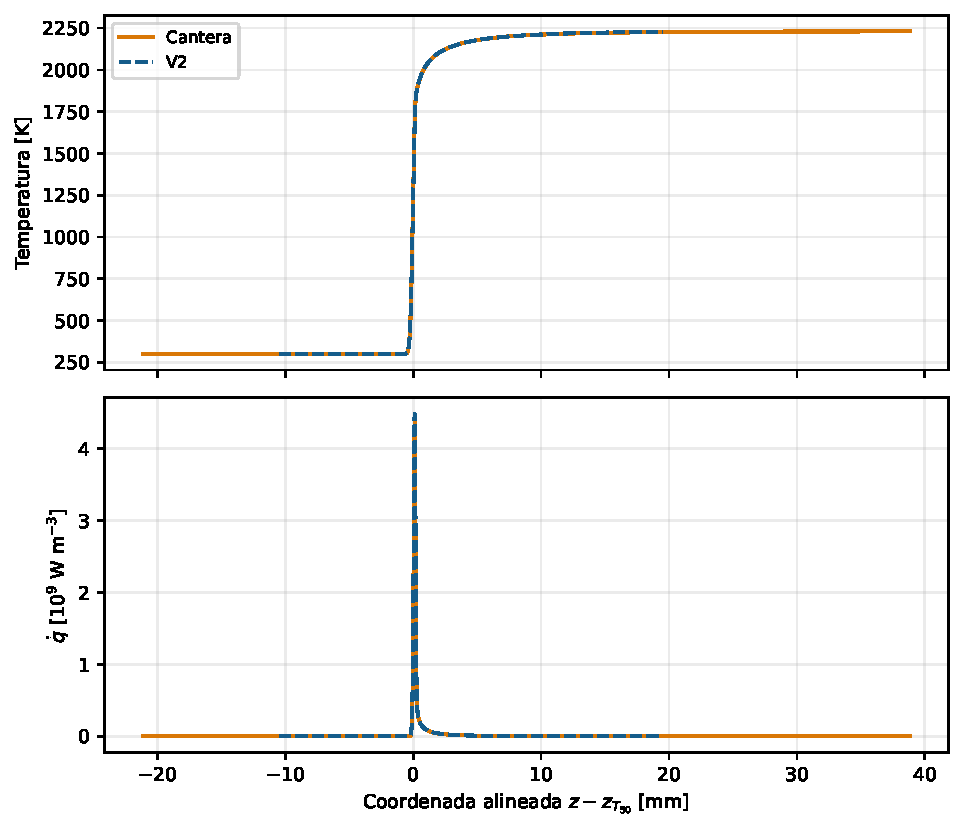
\includegraphics[width=0.98\textwidth]{perfil_estricto_phi1.pdf}
\caption{Perfiles estrictos para \(\phi=1\), alineados por la temperatura media
del salto térmico.}
\label{fig:strict-profile-phi1}
\end{figure}

Los errores de las \cref{eq:error-L2,eq:error-Linf} se evalúan sobre
los perfiles alineados de la figura.
En el caso estequiométrico se obtuvieron \(E_2(T)=\SI{0.0456}{\percent}\),
\(\Delta_\infty(T)=\SI{2.44}{\kelvin}\), \(E_2(\dot q)=\SI{0.602}{\percent}\) y
una diferencia de \(\Su\) de \SI{0.445}{\percent}. El pequeño \(\epsilon\) solo
regulariza campos casi nulos; para especies se acompaña el error relativo con el
error absoluto.

\section{Convergencia de malla y suficiencia del dominio}

Se emplea la medida de sensibilidad espacial definida en la
\cref{eq:mesh-cycle-change}.

Se resolvió el caso estequiométrico desde cero con cuatro niveles de criterio.
La malla ``ultra'' \((2.1,0.02,0.04,0.001)\) es la referencia más fina de esta
secuencia. Todos los casos expandieron el dominio a \SI{0.06}{\metre}.

La \cref{tab:mesh-convergence-pending} reúne las mallas y velocidades de
cada nivel para cuantificar la sensibilidad espacial.

\begin{table}[htbp]
\centering
\caption{Convergencia espacial del caso \(\phi=1\). Los tiempos son ejecuciones
únicas y no constituyen todavía una estadística de rendimiento.}
\label{tab:mesh-convergence-pending}
\begin{tabular}{@{}llrrr@{}}
\toprule
\textbf{Nivel} & \textbf{Solver} & \textbf{Nodos} &
\(\boldsymbol{\Su}\) \textbf{[m/s]} &
\(\boldsymbol{\delta_{\Su}}\) \textbf{[\%]} \\
\midrule
Gruesa & V2 & 109 & 0.3860049 & 2.582 \\
       & Cantera & 105 & 0.3873169 & 2.889 \\
Base   & V2 & 150 & 0.3810358 & 1.262 \\
       & Cantera & 149 & 0.3820550 & 1.491 \\
Estricta & V2 & 261 & 0.3788377 & 0.678 \\
         & Cantera & 275 & 0.3788137 & 0.630 \\
Ultra    & V2 & 505 & 0.3762875 & 0.000 \\
         & Cantera & 517 & 0.3764409 & 0.000 \\
\bottomrule
\end{tabular}
\end{table}

En el nivel ultra, los tiempos de resolución fueron \SI{14.66}{\second}
para V2 y \SI{27.69}{\second} para Cantera. Son observaciones individuales
bajo esta configuración, no una estimación estadística de rendimiento.

La \cref{fig:mesh-convergence-phi1} permite comparar visualmente la
aproximación de ambos solvers al nivel más fino.

\begin{figure}[htbp]
\centering
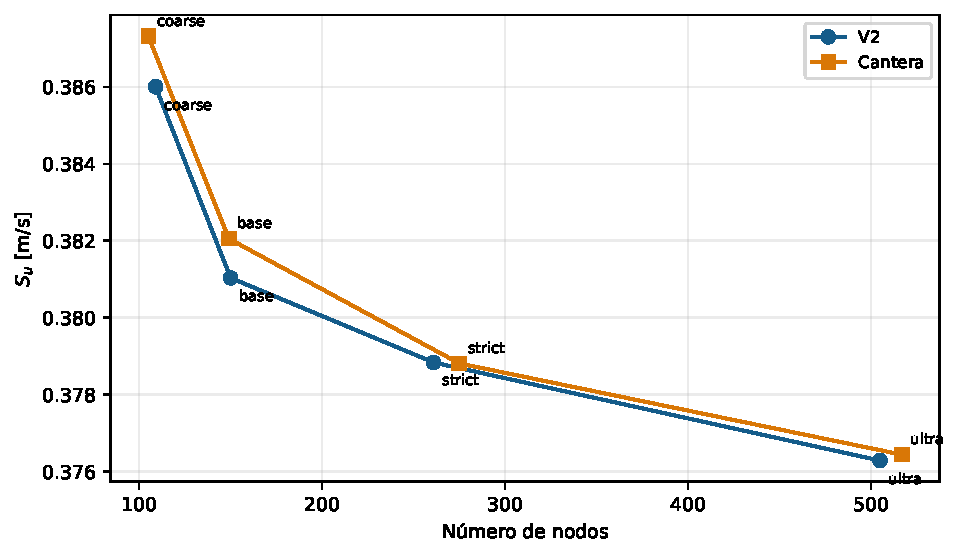
\includegraphics[width=0.90\textwidth]{convergencia_malla_phi1.pdf}
\caption{Velocidad de llama frente al número de nodos para la secuencia de
refinamiento.}
\label{fig:mesh-convergence-phi1}
\end{figure}

La diferencia V2--Cantera es \SI{0.0064}{\percent} en el nivel estricto y
\SI{0.0407}{\percent} en el ultra. Sin embargo, el cambio estricta--ultra de cada
solver aún es aproximadamente \SIrange{0.63}{0.68}{\percent}. Por tanto, la
secuencia demuestra convergencia hacia valores concordantes, pero no justifica
atribuir al nivel estricto una incertidumbre espacial inferior al
\SI{0.1}{\percent}.

El nivel estricto de esta secuencia se obtuvo como llama individual desde frío.
No es la misma trayectoria adaptativa que la fila \(\phi=1\) del barrido: allí
cada solver recibe su propia continuación y termina con 264 y 343 nodos, frente
a 261 y 275 en la ejecución individual. Esta dependencia del camino explica que
la discrepancia de \(\Su\) sea \SI{0.445}{\percent} en el barrido aunque sea
\SI{0.0064}{\percent} en el arranque frío. Lejos de ocultarla, la comparación
refuerza la necesidad de la referencia ultra y de informar malla y semilla junto
con cada resultado.

\section{Conservación y coherencia física}

Las \cref{eq:mass-flow-error,eq:species-sum-error} controlan continuidad y cierre
de composición. En las cinco mezclas estrictas, el peor valor de \(E_m\) fue
\(1.40\times10^{-6}\) para V2 y \(7.35\times10^{-8}\) para Cantera; el peor
\(E_Y\) fue \(4.26\times10^{-10}\) y \(1.96\times10^{-10}\), respectivamente.
La \cref{fig:conservation-sweep} muestra que los errores se mantienen pequeños
en todo el barrido.

\begin{figure}[htbp]
\centering
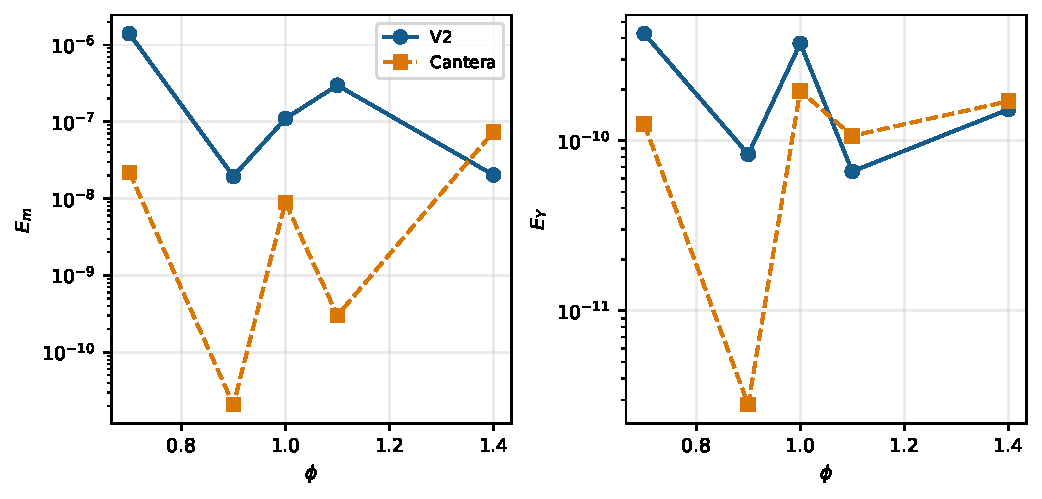
\includegraphics[width=0.91\textwidth]{conservacion_barrido.pdf}
\caption{Errores de flujo másico y suma de fracciones en el barrido estricto.}
\label{fig:conservation-sweep}
\end{figure}

Las pendientes térmicas relativas en ambos bordes quedaron por debajo del
umbral 0.02; el máximo fue 0.00387 en V2 y 0.000734 en Cantera. Entre las cinco
mezclas, el error máximo de perfil fue \(E_2(T)=\SI{0.145}{\percent}\),
\(\Delta_\infty(T)=\SI{6.40}{\kelvin}\) y
\(E_2(\dot q)=\SI{2.52}{\percent}\), todos en \(\phi=1.4\). Estas métricas
complementan a \(\Su\): una velocidad cercana por sí sola no certificaría la
estructura de la llama.

\section{Verificación y rendimiento de la extensión Soret}
\label{sec:soret-verified-results}

\subsection{Verificación de perfiles y balances a una atmósfera}

Una campaña de siete pares alternados para H\(_2\)--aire, GRI-Mech 3.0,
\SI{300}{\kelvin} y \SI{1}{\atmosphere} produjo los resultados de la \cref{tab:soret-native-initial}. Ambas rutas emplearon ratio \(2.5\), slope
\(0.04\), curve \(0.08\) y prune \(0.003\), con aceptación espacial obligatoria.
El coste de \Vdos incluye el arranque nativo con transporte promediado por
mezcla y el corrector final multicomponente/Soret. No se reutilizaron perfiles
persistentes; las cachés de compilación ya estaban preparadas por las pruebas.

\begin{table}[htbp]
\centering
\caption{Verificación inicial con Soret: siete pares alternados. Los tiempos
excluyen la preparación externa del problema.}
\label{tab:soret-native-initial}
\begin{tabular}{@{}lrr@{}}
\toprule
Magnitud & \Vdos & \Cantera\\
\midrule
Mediana de resolución [s] & 8.1535 & 10.4920\\
Cuartiles Q1/Q3 [s] & 7.8790 / 9.2849 & 10.2683 / 10.7651\\
Nodos finales & 207 & 203\\
Dominio final [m] & 0.03 & 0.03\\
\(\Su\) [m/s] & 2.10656035 & 2.10633474\\
Temperatura quemada [K] & 2372.518 & 2371.884\\
\bottomrule
\end{tabular}
\end{table}

La reducción de mediana fue \SI{22.29}{\percent}. El intervalo bootstrap
pareado del \SI{95}{\percent} para el cociente de medianas \Vdos/\Cantera
fue \([0.7463,0.9501]\), con 20000 remuestreos; se conservaron los siete pares,
incluidos los más lentos. La diferencia de \(\Su\) fue
\SI{0.01071}{\percent}. Tras alinear ambos perfiles mediante una temperatura
interior común, las normas \(L_2\) integradas espacialmente dieron errores de
\SI{0.03850}{\percent} en temperatura y \SI{0.08465}{\percent} en liberación
de calor. El máximo entre especies con pico \(Y_k\ge10^{-5}\) fue
\SI{0.54055}{\percent}, para H\(_2\)O\(_2\). El diagnóstico de calor se
reconstruyó mediante \Cantera sobre ambos perfiles, fuera del tiempo medido.

El residual completo final de \Vdos fue 6.7233; el error de suma de fracciones
fue \(1.01\times10^{-12}\) y la variación relativa de flujo másico,
\(2.15\times10^{-10}\). Estos resultados verifican la implementación y una
ventaja temporal en esta campaña. La convergencia del refinador y los gradientes
pequeños en los bordes no sustituyen un estudio independiente de malla y dominio;
tampoco permiten extrapolar el ahorro a otras presiones o mecanismos.

Como comprobación independiente, al reducir slope y curve a \(0.02\) y
\(0.04\), respectivamente, \Vdos obtuvo 390 nodos y
\(\Su=\SI{2.10921829}{\metre\per\second}\); \Cantera obtuvo 386 nodos y
\(\Su=\SI{2.10995877}{\metre\per\second}\). Los tiempos de esta única pareja
fueron \SI{14.29}{\second} y \SI{20.65}{\second}. La discrepancia entre códigos
fue \SI{0.0351}{\percent}, pero el cambio frente a la malla base alcanzó
\SI{0.126}{\percent} y \SI{0.172}{\percent}, respectivamente. Se necesitan más
niveles para establecer un orden observado y una tolerancia de independencia.

El flujo elemental total, reconstruido en caras como convección de punto medio
más difusión, mostró su mayor desviación relativa en el hidrógeno: disminuyó
de \SI{1.644}{\percent} a \SI{0.958}{\percent} en \Vdos y de
\SI{1.617}{\percent} a \SI{0.903}{\percent} en \Cantera al refinar. Esta
reconstrucción es un diagnóstico del balance continuo, no el residual upwind
discreto. Con difusión preferencial no debe confundirse conservación del flujo
elemental con constancia espacial de la fracción elemental.

El control de dominio, iniciado con \SI{0.06}{\metre}, apenas modificó
\(\Su\), pero la temperatura quemada de \Vdos cambió unos
\SI{4.26}{\kelvin}. V2 expandió a \SI{0.12}{\metre} y Cantera conservó
\SI{0.06}{\metre}. Esta sensibilidad exige comprobar también temperatura y
especies lentas, no solamente velocidad. La suficiencia del dominio y el coste
de sus expansiones deben verificarse para cada configuración; los tiempos de
la tabla no se extrapolan a otros dominios iniciales.

\subsection{Comparación del método completo a alta presión}

El método completo combina el transporte nativo con la evaluación química
consistente durante Newton descrita en la \cref{sec:kinetics-newton-treatment}.
La comparación siguiente incluye el coste de la etapa preliminar y del
corrector Soret, con los mismos controles finales de aceptación.

La campaña de alta presión comprendió siete parejas alternadas y empleó slope=0.01,
curve=0.02, ratio=2.5 y prune=0.003 en ambos solvers, con mallas adaptativas
propias. No se reutilizaron perfiles; se conservó la caché de compilación en
disco y se incluyó la primera ejecución. Por tanto, se mide arranque frío
del problema de llama, no compilación completamente fría.
La \cref{tab:soret-signed-kinetics-timing} reúne esta campaña y los controles
complementarios de la misma revisión a una atmósfera. No se mezclan sus tiempos
con los de la verificación inicial: corresponden a campañas distintas.

\begin{table}[htbp]
\centering
\caption{Comparación del método completo con y sin Soret.
Medianas de tiempo de resolución, incluida la etapa preliminar cuando existe.
Los controles de 1 atm conservan slope=0.04 y curve=0.08.}
\label{tab:soret-signed-kinetics-timing}
\begin{tabular}{@{}lrrr@{}}
\toprule
\textbf{Caso} & \textbf{Pares} & \textbf{V2 [s]} & \textbf{Cantera [s]}\\
\midrule
H\(_2\)/Soret, 1 atm & 3 & 5.19 & 9.60\\
CH\(_4\), sin Soret, 1 atm & 3 & 3.80 & 18.92\\
H\(_2\)/Soret, 10 atm, malla fina & 7 & 45.87 & 78.67\\
\bottomrule
\end{tabular}
\end{table}

En el caso fino de \SI{10}{\atmosphere}, las catorce soluciones fueron
aceptadas y cada solver reprodujo exactamente su malla y perfiles entre
repeticiones. La reducción de la mediana fue \SI{41.69}{\percent}; los
cuartiles temporales fueron [44.89,49.86] s para \Vdos y [77.73,79.15] s
para \Cantera. Un bootstrap pareado de 20000 remuestreos dio un intervalo
del 95\% [0.56495,0.66745] para la razón de medianas V2/Cantera.
No se excluyeron las repeticiones lentas.

Los dominios finales fueron de \SI{0.06}{\metre}, con 854 y 868 nodos.
Las velocidades fueron \SI{1.37321383}{\metre\per\second} y
\SI{1.37189618}{\metre\per\second}, diferencia de \SI{0.09605}{\percent}.
Los errores \(E_2\) de perfiles alineados, integrados espacialmente, fueron
\SI{0.004055}{\percent} para temperatura, \SI{0.14283}{\percent} para
liberación de calor y, como máximo entre especies activas,
\SI{0.43261}{\percent} para NO. El residual completo final de \Vdos fue
0.35918, manteniendo la guarda \(10^4\).

La concordancia entre códigos no demuestra por sí sola independencia
espacial. Al pasar de slope=0.02/curve=0.04 al nivel fino, \(\Su\) todavía
cambió aproximadamente \SI{1.18}{\percent} en \Vdos y
\SI{0.84}{\percent} en \Cantera. El error del flujo elemental de hidrógeno
reconstruido en caras fue \SI{0.7145}{\percent} y \SI{0.7501}{\percent},
respectivamente. Se necesita un nivel adicional o extrapolación y control
de dominio para cerrar la incertidumbre espacial. La ventaja temporal queda
demostrada para esta configuración discreta, no para cualquier tolerancia
de error respecto al continuo.

\section{Barrido FGM y efecto de la región de confianza}

Se evaluaron cinco flamelets con
\(\phi=[0.7,0.9,1.0,1.1,1.4]\), refinamiento estricto, caché desactivada y
convergencia de malla obligatoria. Los dos solvers comenzaron con los criterios
estrictos, adaptaron su propia malla y pudieron expandir el dominio. La
\cref{tab:broad-sweep-final} reúne magnitud física, coste y tamaño final sin usar
el residual bruto como indicador de exactitud.

\begin{table}[htbp]
\centering
\caption{Barrido estricto en frío con continuación local. Los tiempos son una
ejecución reproducible.}
\label{tab:broad-sweep-final}
\resizebox{\textwidth}{!}{%
\begin{tabular}{@{}rrrrrrrr@{}}
\toprule
\(\boldsymbol{\phi}\) & \multicolumn{3}{c}{\textbf{V2}} &&
\multicolumn{3}{c}{\textbf{Cantera}}\\
\cmidrule(lr){2-4}\cmidrule(lr){6-8}
& \textbf{Tiempo [s]} & \textbf{Nodos} & \(\boldsymbol{\Su}\) \textbf{[m/s]} &&
\textbf{Tiempo [s]} & \textbf{Nodos} & \(\boldsymbol{\Su}\) \textbf{[m/s]}\\
\midrule
0.7 & 9.57 & 271 & 0.1940860 && 18.36 & 276 & 0.1941428\\
0.9 & 6.64 & 254 & 0.3385254 && 15.55 & 340 & 0.3367645\\
1.0 & 1.14 & 264 & 0.3782542 &&  2.32 & 343 & 0.3765803\\
1.1 & 2.90 & 274 & 0.3815459 &&  4.33 & 344 & 0.3799863\\
1.4 & 8.07 & 259 & 0.1399376 && 20.83 & 396 & 0.1415198\\
\midrule
Suma & 28.32 & -- & -- && 61.38 & -- & --\\
\bottomrule
\end{tabular}}
\end{table}

Los cinco casos \Vdos fueron aceptados. La razón de tiempos exclusivos de
resolución se expresa en la \cref{eq:broad-speedup}:
\begin{equation}
  S_{t,5\phi}=\frac{61.3822}{28.3165}=2.168.
  \label{eq:broad-speedup}
\end{equation}
La \cref{eq:broad-speedup} usa exclusivamente los tiempos de resolución de las
cinco llamas. La diferencia máxima relativa de \(\Su\) fue
\SI{1.118}{\percent}, en \(\phi=1.4\). El resultado temporal del lote es
\(2.17\times\), pero no se generaliza más allá de esta ejecución hasta disponer
de repeticiones alternadas.

\section{Atribución de la mejora}
\label{sec:performance-attribution}

La comparación V2--Cantera recoge la arquitectura completa y no permite asignar
una fracción del ahorro a cada kernel. Para aislar el aporte de la continuación
acotada se repitió el mismo barrido V2 desactivando únicamente
\cref{eq:phi-trust-region}. Todas las demás opciones y criterios de aceptación se
mantuvieron.

La \cref{fig:continuation-ablation} compara el coste de las dos estrategias
para aislar el efecto de acotar la continuación.

\begin{figure}[htbp]
\centering
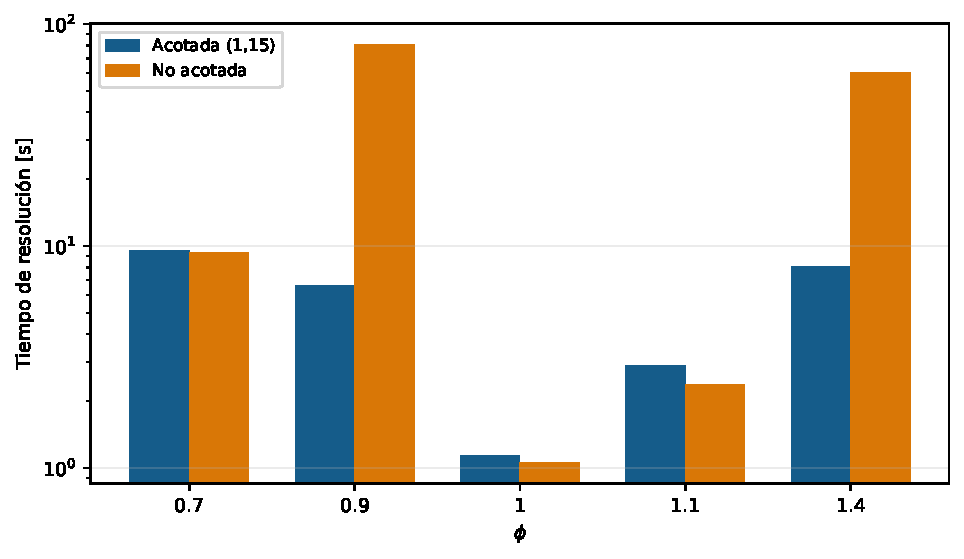
\includegraphics[width=0.91\textwidth]{ablacion_continuacion.pdf}
\caption{Ablación de la región de confianza. La escala logarítmica muestra el
coste concentrado en los saltos \(0.7\to0.9\) y \(1.1\to1.4\).}
\label{fig:continuation-ablation}
\end{figure}

El tiempo acumulado disminuyó de \SI{153.84}{\second} sin límite a
\SI{28.32}{\second} con el radio 1.15: una reducción del
\SI{81.6}{\percent} y una razón interna de \(5.43\times\). En los saltos no
locales, la continuación irrestricta produjo mallas de 325 y 384 nodos y tiempos
de \SI{80.73}{\second} y \SI{60.34}{\second}; el reinicio protegido resolvió los
mismos casos con 254 y 259 nodos en \SI{6.64}{\second} y
\SI{8.07}{\second}. Esta es la mejora causalmente atribuible a la regla de
confianza. El resto de la ventaja frente a Cantera corresponde al conjunto del
solver y no se descompone artificialmente.

\subsection{Ablación de la sustitución por bloques compilada}
\label{sec:block-substitution-ablation}

La segunda ablación mantiene el residual, el Jacobiano, la factorización
pivotada, la continuación y el refinamiento; solo cambia cómo se aplican los
factores a cada lado derecho. La referencia ejecuta una llamada de sustitución
densa por bloque. La variante productiva fusiona el recorrido espacial descrito
en la \cref{eq:block-pivoted-lu} en un kernel compilado. Se ejecutaron dos pares de
barridos completos de cinco llamas, sin caché y con aceptación obligatoria.

La \cref{tab:block-substitution-ablation} resume el coste de ambos modos
de sustitución y permite comprobar su equivalencia física.

\begin{table}[htbp]
\centering
\caption{Ablación pareada de la sustitución lineal. Los tiempos son la suma de
los cinco flamelets; la factorización pivotada es idéntica en ambas rutas.}
\label{tab:block-substitution-ablation}
\begin{tabular}{@{}lrrrr@{}}
\toprule
\textbf{Par} & \textbf{Por bloque [s]} & \textbf{Fusionada [s]} &
\textbf{Reducción [\%]} & \textbf{Aceleración} \\
\midrule
1 & 36.9689 & 33.1981 & 10.20 & 1.114 \\
2 & 37.3083 & 32.1509 & 13.82 & 1.160 \\
\midrule
Mediana & 37.1386 & 32.6745 & 12.02 & 1.137 \\
\bottomrule
\end{tabular}
\end{table}

Todos los flamelets fueron aceptados y cada par terminó con los mismos nodos.
La máxima diferencia absoluta de \(\Su\) fue
\(1.19\times10^{-11}\ \mathrm{m\,s^{-1}}\). Después de proyectar a la tabla
común, las diferencias máximas fueron \SI{0.107}{\kelvin} en temperatura y
\(1.45\times10^{-5}\) en fracción másica. Estas últimas proceden de cambios de
redondeo acumulados durante la trayectoria no lineal y permanecen por debajo de
las discrepancias V2--Cantera documentadas en la verificación de perfiles. La
mejora del \SI{12.0}{\percent} es, por tanto, atribuible al modo de sustitución y
no a una relajación del criterio de aceptación.

Como comprobación temporal independiente de la campaña principal, se intercaló
un barrido Cantera entre dos barridos V2 ya optimizados. Cantera acumuló
\SI{66.70}{\second}; V2 obtuvo \SI{32.15}{\second} antes y
\SI{35.62}{\second} después, con mediana envolvente de
\SI{33.88}{\second} y razón \(1.97\times\). Este ensayo confirma que la ventaja
persiste tras la optimización, pero no se combina con los tiempos de la \cref{tab:broad-sweep-final} ni sustituye las siete repeticiones previstas para
una estimación estadística.

\subsection{Ablación de productos químicos y despacho lineal}
\label{sec:chemical-products-ablation}

Se comparó la combinación de productos químicos especializados de la \cref{eq:small-molecularity-product} y acceso directo a LAPACK con una
referencia que restituye el orden anterior de evaluación química y los
envoltorios lineales anteriores. Cada resolución parte de una conjetura física
sin perfiles guardados. El calentamiento completo se registra por separado y
no se reutiliza como semilla. La \cref{tab:chemical-products-ablation} recoge
siete pares alternados por caso a \SI{1}{\atmosphere}.

\begin{table}[htbp]
\centering
\caption{Ablación interna de V2: medianas de tiempo de resolución a 1 atm.
No es una nueva comparación temporal con Cantera.}
\label{tab:chemical-products-ablation}
\begin{tabular}{@{}lrrr@{}}
\toprule
\textbf{Caso} & \textbf{Anterior [s]} & \textbf{Combinación [s]} &
\textbf{Reducción} \\
\midrule
CH\(_4\), sin Soret & 4.9522 & 4.5983 & \SI{7.15}{\percent} \\
H\(_2\), multicomponente y Soret & 6.9245 & 6.5162 & \SI{5.90}{\percent} \\
\bottomrule
\end{tabular}
\end{table}

Los intervalos bootstrap pareados del \SI{95}{\percent} para la razón de
medianas nueva/anterior fueron \([0.91133,0.95255]\) en metano y
\([0.92865,0.96370]\) en hidrógeno. Las 28 resoluciones medidas fueron
aceptadas, conservaron sus mallas y presentaron diferencias máximas de
temperatura inferiores a \(10^{-8}\) K. La guarda residual se mantuvo en
\(10^4\), sin cambiar las tolerancias ni el refinamiento. Estos ensayos
demuestran una mejora de implementación sobre los casos comparados, no una
nueva formulación física ni independencia de malla. El porcentaje combinado
no puede atribuirse íntegramente a LAPACK ni sumarse a aceleraciones de otras
campañas.

Una confirmación exploratoria adicional empleó tres pares H\(_2\)/Soret a
\SI{10}{\atmosphere}, con slope=0.01 y curve=0.02. Las medianas fueron
\SI{53.9952}{\second} para la referencia anterior y \SI{48.0511}{\second}
para la combinación, una reducción del \SI{11.01}{\percent}. Las seis
resoluciones conservaron 854 nodos y fueron aceptadas; la diferencia máxima
de temperatura fue inferior a \(3\times10^{-10}\) K. El intervalo bootstrap
pareado de la razón fue \([0.88274,0.90347]\), pero tres pares no sustituyen
una campaña estadística más amplia ni cierran la independencia espacial.

Una pareja directa posterior, con esa misma configuración a 10 atm, obtuvo
\SI{46.85}{\second} para \Vdos y \SI{81.79}{\second} para \Cantera,
con 854 y 868 nodos respectivamente y discrepancia de \(\Su\) del
\SI{0.09605}{\percent}. Este control individual no reemplaza la comparación
estadística ni permite mezclar sus tiempos con las medianas de otras campañas.



\subsection{Ablación del refresco local certificado}
\label{sec:local-refresh-ablation}

El refresco de la \cref{sec:local-jacobian-refresh} se evaluó como una ablación
del corrector, no como una comparación fría V2--Cantera. Se usó
CH\(_4\)--aire con GRI-Mech~3.0, \SI{300}{\kelvin}, \SI{10}{\atmosphere} y
las dos transiciones locales \(\phi=1.00\rightarrow1.02\rightarrow1.04\).
Se alternaron siete pares con y sin el rescate, manteniendo el mismo predictor
tangente, la malla, el certificado y la guarda operacional
\(\norm{\vect F}_\infty\le10^4\). Así se aísla el coste de corregir un modelo
lineal envejecido de la diferencia entre dos soluciones físicas o de la
variabilidad de un arranque frío.

La \cref{tab:local-refresh-ablation} presenta los tiempos pareados del
corrector con y sin refresco selectivo, manteniendo el mismo certificado.

\begin{table}[htbp]
\centering
\caption{Ablación pareada del refresco local certificado en transiciones FGM a
alta presión. La razón es tiempo sin refresco dividido por tiempo con refresco.}
\label{tab:local-refresh-ablation}
\begin{tabular}{@{}p{0.43\textwidth}p{0.42\textwidth}@{}}
\toprule
\textbf{Magnitud} & \textbf{Resultado} \\
\midrule
Pares alternados & 7 \\
Transiciones por par & \(1.00\rightarrow1.02\rightarrow1.04\) \\
Mediana de la razón temporal & \(2.023\times\) \\
IC bootstrap pareado al \SI{95}{\percent} & \([1.943,\,2.056]\) \\
Pares que conservaron certificación & 7 de 7 \\
Actividad del rescate & 79 bloques actualizados en dos eventos por barrido \\
Máxima diferencia frente al baseline &
\(\Delta\Su=1.36\times10^{-8}\),
\(E_2(T)=2.10\times10^{-9}\),
\(E_2(Y)=3.94\times10^{-8}\),
\(E_2(\dot q)=6.23\times10^{-8}\) \\
\bottomrule
\end{tabular}
\end{table}

La \cref{tab:local-refresh-ablation} demuestra una mejora pareada del
corrector en la región donde el defecto de linealización se activa, sin un
cambio medible de la solución certificada. En una transición análoga a
\SI{1}{\atmosphere} el indicador no seleccionó bloques y ambas rutas produjeron
perfiles idénticos; esa inactividad es deseable, porque evita pagar un rescate
cuando la linealización ya es suficiente. La evidencia no autoriza afirmar una
aceleración universal a \SI{10}{\atmosphere}, ni reemplaza una comparación fría
con Cantera: su conclusión acotada es que el defecto local puede identificar un
refresco rentable dentro de una continuación paramétrica certificada.

\section{Validación de la tabla FGM}

La tabla demostrativa contiene cinco filas en \(Z\), 241 nodos comunes en \(c\)
y las 53 especies de GRI-Mech 3.0. Después de interpolar, el máximo error de
suma de fracciones fue \(4.26\times10^{-10}\) en V2 y
\(1.96\times10^{-10}\) en Cantera. Esta comprobación demuestra consistencia
estructural, pero no mide resolución entre filas.

Para ello se retiraron sucesivamente \(\phi=0.9,1.0,1.1\) y cada perfil se
reconstruyó linealmente con sus vecinos. La \cref{tab:fgm-cross-validation}
recoge la validación cruzada de la tabla V2.

\begin{table}[htbp]
\centering
\caption{Error de exclusión de una mezcla interior en la tabla V2.}
\label{tab:fgm-cross-validation}
\resizebox{\textwidth}{!}{%
\begin{tabular}{@{}rrrrr@{}}
\toprule
\(\boldsymbol{\phi}\) & \(\boldsymbol{E_2(T)}\) \textbf{[\%]} &
\(\boldsymbol{E_2(\dot q)}\) \textbf{[\%]} &
\(\boldsymbol{E_2(\dot\omega_c)}\) \textbf{[\%]} &
\(\boldsymbol{\max|\Delta Y_k|}\) \\
\midrule
0.9 & 1.605 & 5.602 & 8.897 & 0.00621 \\
1.0 & 2.036 & 11.541 & 11.137 & 0.00996 \\
1.1 & 2.907 & 27.891 & 26.251 & 0.00561 \\
\bottomrule
\end{tabular}}
\end{table}

La \cref{fig:fgm-cross-validation} muestra dónde se concentra el error al
reconstruir una mezcla que no intervino en la interpolación.

\begin{figure}[htbp]
\centering
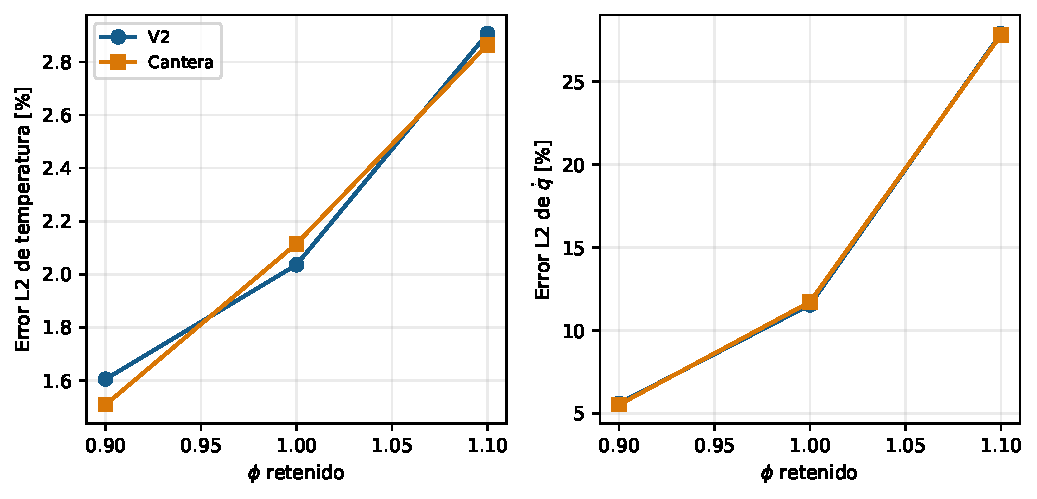
\includegraphics[width=0.90\textwidth]{validacion_cruzada_fgm.pdf}
\caption{Error de validación cruzada al retener mezclas interiores.}
\label{fig:fgm-cross-validation}
\end{figure}

El error de \(\dot q\) alcanza \SI{27.9}{\percent}, con un comportamiento casi
idéntico en la tabla construida desde Cantera. La limitación es, por tanto, la
separación de las filas en \(Z\), no el solver que generó los flamelets. La tabla
de cinco mezclas valida el flujo de trabajo y el contrato de datos, pero no debe
emplearse como cierre de una simulación CFD. Una tabla de producción requiere
muestreo adaptativo en \(Z\) hasta cumplir una tolerancia de validación externa.

% =============================================================================
\chapter{Discusión}
\label{chap:discusion}

\section{Cumplimiento de los objetivos y fidelidad numérica}

La evidencia obtenida permite responder al objetivo principal dentro del régimen
estudiado. \Vdos reproduce la velocidad de llama y los perfiles de \Cantera con
diferencias pequeñas una vez que ambos solvers se comparan bajo el mismo modelo
y con resolución espacial suficiente. En el nivel ultra del caso
estequiométrico, la diferencia de \(\Su\) fue de \SI{0.041}{\percent}; en el
barrido de cinco mezclas, los errores máximos alineados fueron
\SI{0.145}{\percent} en temperatura y \SI{2.52}{\percent} en liberación de
calor. Estas cifras no prueban exactitud experimental, pero sí muestran que la
comparación temporal se realiza entre soluciones numéricamente coherentes con la
misma física de referencia.

La secuencia de malla también revela una limitación importante: una diferencia
pequeña entre dos códigos no implica por sí sola independencia del continuo. El
cambio entre los niveles estricto y ultra permanece del orden de
\SIrange{0.63}{0.68}{\percent} en \(\Su\). Por tanto, la concordancia entre
solvers y la convergencia espacial se tratan como pruebas complementarias y no
como sustitutas. Esta separación responde directamente al criterio metodológico
de medir rendimiento solo después de establecer la calidad de la solución.

\section{Origen de la reducción del tiempo de cálculo}

La reducción temporal observada no puede atribuirse a una única optimización.
El tiempo extremo a extremo incluye la trayectoria no lineal, la construcción y
reutilización del Jacobiano, la evaluación termoquímica, la adaptación de malla
y, en los barridos, la selección de la semilla. Por ello, la comparación global
\Vdos--\Cantera caracteriza la arquitectura completa y no debe descomponerse en
porcentajes independientes.

Las ablaciones permiten aislar algunas causas. La sustitución compilada por
bloques reduce el coste repetitivo sin modificar la factorización ni el sistema
lineal, mientras que la región de confianza actúa sobre una fuente distinta de
coste: evita que una solución convergida pero paramétricamente lejana se convierta
en una mala semilla. El resultado de esta última ablación es especialmente
relevante porque muestra que \emph{reutilizar más información no siempre reduce
el tiempo}. La continuación solo es beneficiosa cuando la proximidad paramétrica
compensa el coste de corregir el predictor.

El refresco local del Jacobiano responde a la misma lógica de especialización.
Cuando el defecto de linealización está confinado, actualizar únicamente una
región puede rescatar el corrector sin relajar el certificado final. La evidencia
disponible demuestra esta ventaja en las transiciones evaluadas, pero no permite
convertirla en una afirmación general sobre arranques fríos o mecanismos de otro
tamaño.

\section{Relación con trabajos previos}

Los resultados no contradicen las ventajas de álgebra dispersa y métodos
iterativos reportadas por Lapointe et al. y Perini et al.
\cite{Lapointe2019,Perini2025}. Esos trabajos incluyen mecanismos que alcanzan
centenares o miles de especies, régimen en el que la construcción, almacenamiento
y solución del Jacobiano adquieren un peso creciente. GRI-Mech~3.0 contiene 53
especies y sitúa el presente estudio en un equilibrio computacional diferente.
La observación de Wu et al. de que la estrategia lineal óptima cambia con el
tamaño del mecanismo refuerza esta interpretación \cite{Wu2023}.

En consecuencia, la resolución directa tridiagonal por bloques no se propone
como alternativa universal a GMRES, KLU u otros solvers dispersos. Se presenta
como una decisión adecuada para el régimen medido, donde los bloques siguen
siendo lo bastante pequeños para que el coste y la sobrecarga de una
infraestructura iterativa no estén necesariamente amortizados. Una extensión
hacia mecanismos grandes deberá determinar experimentalmente el punto en que
este equilibrio cambia.

El mismo criterio se aplica a la continuación. Perini et al. muestran que partir
de una solución previamente convergida puede resultar desfavorable si arrastra
una malla refinada hacia una condición suficientemente diferente
\cite{Perini2025}. La región de confianza de este trabajo proporciona una
respuesta simple y reproducible a ese problema: solo reutiliza información en
un entorno local y vuelve al arranque físico fuera de él. La contribución no es
la idea genérica de continuar, sino medir y proteger su dominio de utilidad.

\section{Implicaciones para la generación FGM}

La aplicación FGM convierte una mejora por llama en una reducción acumulada,
pero introduce una segunda fuente de error: la discretización del espacio de
parámetros. La validación por exclusión mostró que una tabla puede ser
estructuralmente correcta y, al mismo tiempo, estar insuficientemente resuelta
en \(Z\). El error de hasta \SI{27.9}{\percent} en liberación de calor impide
presentar las cinco mezclas actuales como una tabla lista para CFD.

Este resultado es metodológicamente útil porque separa dos preguntas que suelen
confundirse. La primera es si el solver produce flamelets correctos; la segunda,
si existen suficientes flamelets para interpolar el manifold. Mejorar el solver
no elimina la necesidad de muestreo paramétrico, y añadir filas a la tabla no
corrige una llama individual mal resuelta. La siguiente extensión natural es,
por tanto, un muestreo adaptativo que inserte flamelets donde la validación
identifique error elevado.

\section{Extensión multicomponente con Soret}

Los resultados de hidrógeno--aire muestran que la arquitectura puede extenderse
a una física de transporte más exigente. La concordancia de velocidad y perfiles
con \Cantera, junto con las campañas pareadas de tiempo, constituye evidencia
favorable para la implementación. Sin embargo, la sensibilidad espacial a alta
presión todavía impide atribuir una incertidumbre de continuo comparable a la
del caso base. La afirmación correcta es, por tanto, que la ruta
multicomponente/Soret ha sido implementada y comparada con éxito en los casos
reportados, no que esté validada para todo el dominio de hidrógeno.

Esta limitación también ilustra por qué el rendimiento debe acompañarse de una
métrica de error. Una configuración puede ser más rápida sobre una malla dada y
seguir necesitando más refinamiento para alcanzar una tolerancia espacial más
estricta. El objetivo futuro debe ser minimizar el tiempo hasta una solución con
error controlado, no solamente el tiempo de una discretización fija.

\section{Limitaciones y amenazas a la validez}

La primera limitación es estadística. Algunos tiempos de la campaña principal de
metano proceden de una única ejecución y se identifican explícitamente como
preliminares; una comparación definitiva requiere repeticiones alternadas para
reducir el efecto de frecuencia de CPU, cachés y carga del sistema. Las
ablaciones y campañas Soret que sí disponen de pares repetidos se interpretan de
forma separada.

La segunda limitación es de equivalencia numérica. Los dos solvers adaptan su
propia malla, por lo que imponer los mismos criterios no produce necesariamente
los mismos nodos. Esta diferencia forma parte de la pregunta de tiempo hasta
aceptación, pero exige reportar simultáneamente malla, dominio y errores de
perfil. Una comparación sobre una malla idéntica solo se utiliza cuando se desea
aislar una operación concreta.

La tercera limitación es de generalización. Los resultados principales se
obtienen con GRI-Mech~3.0 y no permiten extrapolar el balance entre álgebra
directa e iterativa hacia mecanismos grandes. Del mismo modo, la comparación
con \Cantera es una validación numérica independiente, no una validación
experimental del mecanismo químico. El error de modelo, el error de transporte
y el error numérico deben mantenerse conceptualmente separados.

\section{Sostenibilidad e implicaciones del trabajo}

La contribución a la sostenibilidad se sitúa principalmente en el uso eficiente
de recursos computacionales. Reducir el tiempo necesario para generar una
familia de llamas o una tabla termoquímica disminuye potencialmente el consumo de
CPU asociado a campañas paramétricas y permite explorar más condiciones con la
misma infraestructura. No obstante, este TFM mide tiempo de ejecución y no
energía eléctrica; por ello, no se asume una reducción energética proporcional
al \emph{speedup}.

Desde una perspectiva aplicada, una generación termoquímica más eficiente puede
facilitar estudios de combustibles alternativos y diseños orientados a menores
emisiones, pero esa consecuencia no se cuantifica aquí. Una extensión rigurosa
consistiría en registrar energía por llama aceptada y energía por tabla generada,
de modo que la eficiencia computacional pueda evaluarse también en términos
ambientales y económicos.

\section{Síntesis de la discusión}

La evidencia disponible apoya una conclusión acotada: para el régimen estudiado,
la especialización de la estructura 1D, la globalización y la reutilización
paramétrica controlada reducen el trabajo necesario para alcanzar soluciones
aceptadas sin introducir diferencias materiales frente a la referencia. La
fuerza del resultado reside tanto en las mejoras positivas como en los casos en
que una estrategia deja de ser conveniente. Esta lectura evita una afirmación de
superioridad universal y convierte el TFM en una evaluación causal del régimen
en el que cada decisión numérica resulta útil.

% =============================================================================
\chapter{Conclusiones y trabajo futuro}
\label{chap:conclusiones}

\section{Conclusiones}

Este TFM desarrolló y evaluó una metodología especializada para resolver
familias de llamas premezcladas laminares unidimensionales y utilizarlas en la
generación de tablas FGM. La evaluación se planteó desde el inicio sobre una
condición: toda comparación temporal debía realizarse entre soluciones que
superaran criterios explícitos de convergencia no lineal, conservación,
resolución espacial y coherencia física. Bajo ese criterio, los resultados
permiten establecer las siguientes conclusiones:

\begin{enumerate}
  \item La formulación de llama libre debe resolver conjuntamente el flujo
        másico, la temperatura y la composición, mientras una condición de
        anclaje elimina únicamente la indeterminación por traslación. Esta
        formulación permite recuperar \(\Su\) como parte de la solución sin
        prescribirla externamente.

  \item La localidad espacial del problema produce un Jacobiano tridiagonal por
        bloques que puede explotarse de forma directa en el régimen estudiado.
        Mantener la factorización pivotada y fusionar las sustituciones repetidas
        redujo la mediana del barrido de \SI{37.14}{\second} a
        \SI{32.67}{\second}, sin modificar de forma material la malla ni la
        velocidad de llama.

  \item La combinación de Newton amortiguado, PTC--SER y rescate por Euler
        implícito proporciona una jerarquía de globalización en la que las
        correcciones baratas se intentan antes de resolver un paso
        pseudo-transitorio completo. La mejora se evalúa sobre el tiempo hasta
        aceptación y no únicamente sobre el coste de una operación lineal.

  \item Para metano--aire con GRI-Mech~3.0, \Vdos reproduce la referencia con
        diferencias pequeñas una vez controlada la resolución espacial. En el
        nivel ultra del caso estequiométrico, las velocidades fueron
        \SI{0.376287}{\metre\per\second} y
        \SI{0.376441}{\metre\per\second} para \Vdos y \Cantera,
        respectivamente, una diferencia de \SI{0.041}{\percent}.

  \item En el barrido frío de cinco mezclas, el tiempo acumulado fue
        \SI{28.32}{\second} para \Vdos y \SI{61.38}{\second} para
        \Cantera. Esta comparación muestra una ventaja en la configuración
        medida, pero se mantiene como resultado temporal preliminar hasta
        completar repeticiones alternadas.

  \item La continuación paramétrica debe utilizarse de forma local. Eliminar
        la región de confianza elevó el tiempo acumulado del barrido desde
        \SI{28.32}{\second} hasta \SI{153.84}{\second}. Por tanto, una
        solución previamente convergida no constituye automáticamente una buena
        semilla para una condición suficientemente distante.

  \item La extensión multicomponente con Soret mostró concordancia favorable
        con \Cantera en los casos de hidrógeno evaluados y una reducción
        temporal en las campañas pareadas. Sin embargo, la sensibilidad espacial
        a alta presión todavía debe cerrarse antes de generalizar la precisión
        de esta ruta.

  \item La cadena FGM separa correctamente la calidad del flamelet de la
        resolución del manifold. La validación por exclusión alcanzó un error de
        hasta \SI{27.9}{\percent} en liberación de calor con cinco mezclas, por
        lo que la tabla actual demuestra el flujo de generación, pero no puede
        presentarse todavía como una tabla de producción para CFD.
\end{enumerate}

En conjunto, la contribución principal es una arquitectura reproducible para
reducir el tiempo extremo a extremo de obtener una llama aceptada y reutilizarla
de forma controlada dentro de una familia. La evidencia no sustenta una
superioridad universal frente a solvers generales ni permite extrapolar el
resultado a mecanismos cinéticos grandes; sí delimita un régimen en el que la
especialización de la estructura 1D y la continuidad paramétrica aportan una
ventaja medible.

\section{Trabajo futuro}

Las siguientes extensiones se desprenden directamente de las limitaciones
identificadas:

\begin{enumerate}
  \item completar repeticiones alternadas de las campañas temporales para
        reportar medianas e intervalos de incertidumbre en todos los casos;
  \item ampliar la verificación espacial y física al variar temperatura,
        presión, combustible y mecanismo;
  \item estudiar mecanismos cinéticos progresivamente mayores para localizar el
        régimen en que la resolución directa por bloques deja de ser competitiva
        frente a álgebra dispersa y métodos iterativos precondicionados;
  \item completar la campaña del predictor--corrector adaptativo y compararla
        con arranque frío, región fija y puentes fijos bajo el mismo certificado;
  \item introducir muestreo adaptativo en \(Z\) y añadir flamelets hasta que
        la validación por exclusión satisfaga una tolerancia previamente fijada;
  \item ampliar la validación multicomponente/Soret y separar con mayor detalle
        error de transporte, error de discretización y error del mecanismo;
  \item incorporar medidas de energía consumida por llama aceptada para
        complementar el tiempo de pared con una métrica directa de eficiencia
        computacional.
\end{enumerate}

\subsection{Evaluación pendiente del control de paso paramétrico}
\label{sec:future-adaptive-pc}

El controlador de paso implementado como opción propone un punto en \(\ell\), corrige la
llama completa con la cadena Newton--PTC--BE y aplica exactamente el predicado de
aceptación de la \cref{eq:acceptance-predicate}. Tras una corrección aceptada, el
defecto del predictor se mide mediante la \cref{eq:predictor-corrector-defect} sobre la malla final:
\begin{equation}
  \eta_p=\left[\frac{1}{Nn_v}\sum_{j,v}
  \left(\frac{x_{j,v}^*-x_{j,v}^{\mathrm{pred}}}
  {\varepsilon_{a,v}+\varepsilon_{r,v}\,\overline{\abs{x_v^*}}}\right)^2
  \right]^{1/2}.
  \label{eq:predictor-corrector-defect}
\end{equation}
La normalización de la \cref{eq:predictor-corrector-defect} coincide con la usada
para las correcciones no lineales y evita atribuir un defecto grande únicamente a
las unidades de temperatura o a una especie traza.

El paso \(\Delta\ell\) se inicia en \(\log(1.15)\), se limita a
\([\log(1.02),\log(1.20)]\) y, después de tres defectos secantes aceptados,
usa su mediana \(\eta_{\rm ref}\) para actualizarse mediante la \cref{eq:adaptive-continuation-step}:
\begin{equation}
  \Delta\ell_{i+1}=\operatorname{clip}\left[
  \Delta\ell_i\operatorname{clip}\left(
  0.9\sqrt{\frac{\eta_{\rm ref}}{\max(\eta_p,\epsilon)}},0.5,1.25\right),
  \log(1.02),\log(1.20)\right].
  \label{eq:adaptive-continuation-step}
\end{equation}
Si el corrector falla, el estado de prueba no se guarda: se conserva el último
flamelet certificado, se reduce el paso y se reintenta. Tras cuatro rechazos o
al alcanzar el paso mínimo, se resuelve el objetivo mediante un arranque frío y
se registra explícitamente la recuperación. Un defecto alto de un flamelet
certificado reduce solo el paso posterior; no invalida una solución física.

Cuando un objetivo solicitado requiere varios pasos, los puntos puente se
incorporan como filas adicionales del manifold y quedan marcados de forma
explícita. La traza de cada intento conserva parámetros inicial, objetivo y
prueba, predictor empleado, defecto, refinamientos, expansiones de dominio,
tiempo, aceptación, reintentos y paso siguiente. Por tanto, la caché acelera una
semilla pero no sustituye ni la corrección ni la certificación.

La comparación del predictor--corrector adaptativo frente al arranque frío,
la región fija y los puentes fijos no forma parte de la evidencia cerrada de
este TFM. Su evaluación se mantiene como trabajo futuro y, por tanto, no se le
atribuye ninguna ganancia temporal en los resultados.

Para el muestreo paramétrico futuro, un criterio posible es estimar el error de
interpolación en cada intervalo mediante la \cref{eq:parametric-adaptivity}:
\begin{equation}
  \eta_i=\max_{q\in\mathcal{Q}}
  \frac{\norm{q_{\mathrm{mid}}-\mathcal{I}(q_i,q_{i+1})}}
  {s_q},
  \label{eq:parametric-adaptivity}
\end{equation}
y añadir un flamelet únicamente cuando \(\eta_i\) supere la tolerancia
establecida. De esta forma, el número de soluciones deja de fijarse a priori y
pasa a estar determinado por la evidencia de interpolación.

\section{Cierre}

El desarrollo muestra que acelerar una llama unidimensional no consiste en
seleccionar de forma aislada un solver lineal o una estrategia de continuación.
El rendimiento surge de la interacción entre formulación, estructura algebraica,
globalización, adaptación espacial, evaluación termoquímica y elección de
semillas. Al evaluar esas decisiones sobre soluciones previamente certificadas,
el trabajo proporciona una base reproducible para extender el estudio hacia
mecanismos mayores y manifolds FGM con resolución paramétrica controlada.

% =============================================================================
\appendix
\chapter{Configuración, tolerancias y trazabilidad}
\label{app:configuracion}

\section{Caso base}

La \cref{tab:base-physical-config} reúne la configuración que acompaña a todos
los resultados de referencia.

\begin{longtable}{@{}p{0.34\textwidth}p{0.24\textwidth}p{0.30\textwidth}@{}}
\caption{Configuración física de referencia.}
\label{tab:base-physical-config}\\
\toprule
\textbf{Parámetro} & \textbf{Valor} & \textbf{Observación} \\
\midrule
\endfirsthead
\toprule
\textbf{Parámetro} & \textbf{Valor} & \textbf{Observación} \\
\midrule
\endhead
Mecanismo & GRI-Mech 3.0 & 53 especies; validar archivo exacto. \\
Combustible & CH\(_4\) & Composición pura en el caso base. \\
Oxidante & aire & Composición definida en el comando/configuración. \\
Temperatura de entrada & \SI{300}{\kelvin} & Uniforme en corriente fresca. \\
Presión & \SI{1}{\atmosphere} & Constante. \\
Ancho inicial & \SI{0.03}{\metre} & Expandible si el borde no es plano. \\
Transporte & mixture-averaged & Gradiente molar corregido. \\
Soret & desactivado & Activarlo para H\(_2\) requiere nueva validación. \\
Malla inicial & 8 nodos & Bootstrap fijo intermedio desactivado. \\
\bottomrule
\end{longtable}

\section{Parámetros no lineales}

Los valores productivos y su justificación se registran en la \cref{tab:nonlinear-config}.

\begin{longtable}{@{}p{0.38\textwidth}p{0.18\textwidth}p{0.32\textwidth}@{}}
\caption{Parámetros productivos del solver no lineal.}
\label{tab:nonlinear-config}\\
\toprule
\textbf{Parámetro} & \textbf{Valor} & \textbf{Justificación} \\
\midrule
\endfirsthead
\toprule
\textbf{Parámetro} & \textbf{Valor} & \textbf{Justificación} \\
\midrule
\endhead
Tolerancia estacionaria relativa & \(10^{-4}\) & Compatible con aceptación base. \\
Tolerancia estacionaria absoluta & \(10^{-9}\) & Protege especies pequeñas. \\
Tolerancia transitoria relativa & \(10^{-4}\) & Misma escala relativa. \\
Tolerancia transitoria absoluta & \(10^{-11}\) & Mayor exigencia en rescate. \\
Norma ponderada de paso & \(<1\) & Criterio principal con guarda residual. \\
Máximo de damping & 7 & Factor entre niveles \(\sqrt{2}\). \\
Edad máxima de Jacobiano & 20 & Valor fijo en todos los casos comparativos. \\
Factor SER & 1.1 & Valor fijo en todos los casos comparativos. \\
Clip SER & \([0.2,5.0]\) & Limita cambios extremos. \\
Crecimiento residual permitido & 10 & Rechaza correcciones divergentes. \\
Solver lineal & Tridiagonal por bloques híbrido & Factorización pivotada de los
bloques con LAPACK y sustituciones fusionadas compiladas, sin formar inversas. \\
\bottomrule
\end{longtable}

\section{Refinamiento y dominio}

La \cref{tab:refinement-config} separa la fase base de la fase estricta.

\begin{table}[htbp]
\centering
\caption{Criterios de refinamiento usados en la comparación estricta.}
\label{tab:refinement-config}
\begin{tabular}{@{}lrrrr@{}}
\toprule
\textbf{Etapa} & \textbf{Ratio} & \textbf{Slope} & \textbf{Curve} &
\textbf{Prune} \\
\midrule
Base & 3.0 & 0.08 & 0.12 & 0.010 \\
Estricta & 2.5 & 0.04 & 0.08 & 0.003 \\
\bottomrule
\end{tabular}
\end{table}

Se permiten seis ciclos adaptativos. El dominio puede duplicarse con factor 2
hasta el límite configurado; la pendiente relativa de borde de referencia es
0.02. Estos valores deben figurar junto a cualquier tiempo, porque una malla no
convergida puede parecer artificialmente rápida.

\section{Continuación paramétrica}

La referencia fija usa la razón máxima de \SI{15}{\percent} de la \cref{eq:phi-trust-region}. El predictor--corrector adaptativo conserva esa
escala como paso inicial, pero controla el paso en \(\log\phi\) y registra cada
intento. La \cref{tab:continuation-config} documenta la opción adaptativa de la
\cref{sec:future-adaptive-pc}, cuya evaluación comparativa permanece pendiente.

\begin{table}[htbp]
\centering
\caption{Parámetros del controlador de paso adaptativo pendiente de evaluación.}
\label{tab:continuation-config}
\begin{tabularx}{\textwidth}{@{}p{0.34\textwidth}p{0.18\textwidth}Y@{}}
\toprule
\textbf{Parámetro} & \textbf{Valor} & \textbf{Función} \\
\midrule
Coordenada & \(\ell=\log\phi\) & Hace simétricos los cambios
multiplicativos de mezcla. \\
Paso inicial & \(\log(1.15)\) & Reproduce la escala de la región fija como
condición inicial. \\
Intervalo de paso & 1,02--1,20 & Evita tanto saltos
no locales como subdivisiones inútiles. \\
Referencia de defecto & Mediana de 3 secantes & Evita fijar una escala de
error dependiente de un único combustible. \\
Factor de seguridad / clip & \(0.9\), \([0.5,1.25]\) & Limita la variación
del paso entre correcciones. \\
Máximo de rechazos & 4 & Activa un arranque frío trazable, no una semilla
oculta. \\
Filas puente & Sí & Aumentan la resolución paramétrica de la tabla y quedan
marcadas en sus metadatos. \\
\bottomrule
\end{tabularx}
\end{table}

\section{Variables de entorno}

La \cref{tab:thread-config} documenta el reparto de hilos y procesos de la
máquina de referencia.

\begin{table}[htbp]
\centering
\caption{Control de paralelismo en la máquina de referencia.}
\label{tab:thread-config}
\begin{tabularx}{\textwidth}{@{}p{0.30\textwidth}p{0.18\textwidth}Y@{}}
\toprule
\textbf{Variable/opción} & \textbf{Base} & \textbf{Motivo} \\
\midrule
\codigo{OPENBLAS\_NUM\_THREADS} & 1 & Evitar coste de hilos en bloques densos
pequeños. \\
\codigo{NUMBA\_NUM\_THREADS} & 4 & Mejor resultado del kernel secuencial en
la máquina medida. \\
Hilos de química por proceso & automático/4 & Permite repartir el trabajo
entre procesos FGM sin sobreparalelismo. \\
Número de procesos & 1 frío; hasta \(N_\phi\) cacheado & Conservar continuación
fría y explotar independencia cacheada. \\
\bottomrule
\end{tabularx}
\end{table}

Numba compila funciones numéricas a través de LLVM \cite{LamNumba2015}; SciPy
proporciona acceso a rutinas lineales optimizadas \cite{VirtanenSciPy2020}. Las
versiones exactas forman parte del entorno experimental y deben conservarse con
cualquier campaña que pretenda comparar tiempos.

\section{Reglas de cambio de configuración}

Para impedir que una aceleración rompa silenciosamente la solución, toda
modificación productiva debe superar:

\begin{enumerate}
  \item pruebas unitarias de propiedades y conservación;
  \item misma llama sobre malla fija, con diferencias cercanas al redondeo cuando
        el cambio pretende ser algebraicamente equivalente;
  \item barrido FGM frío con aceptación completa;
  \item comparación de \(\Su,T,\dot q,Y_k\) y nodos;
  \item al menos cinco repeticiones alternadas de tiempo;
  \item actualización del registro de decisiones.
\end{enumerate}

Una mejora que cambia ligeramente la trayectoria puede terminar en otra malla
igualmente válida. En ese caso no se exige identidad bit a bit; se exige
convergencia de malla y error físico cuantificado.

\chapter{Reproducción de resultados y formato de datos}
\label{app:reproducibilidad}

\section{Procedimiento reproducible}

La campaña se ejecuta desde dos puntos de entrada equivalentes: uno resuelve con
V2 y otro con \codigo{FreeFlame}. Ambos reciben la misma lista de \(\phi\), el
mismo mecanismo, transporte, criterios de malla y resolución \((Z,c)\), y ambos
usan el mismo posprocesado. Cada ejecución guarda argumentos, versiones, tiempos,
estado de aceptación, perfiles nodales y tabla final. Un tercer proceso de
análisis lee esos archivos, alinea los frentes y produce las métricas y figuras
del \cref{chap:resultados}. Los comandos literales permanecen junto a los
generadores para evitar que la tesis dependa de una sintaxis de interfaz. En
continuación adaptativa se añade una traza estructurada por intento: parámetros
inicial, objetivo y prueba, predictor, defecto, refinamiento, dominio,
aceptación, recuperación y paso siguiente. Así se puede reproducir la ruta, no
solo sus resultados finales.

\section{Lista de comprobación antes de medir}

\begin{enumerate}
  \item Guardar la revisión y el estado del árbol de trabajo.
  \item Registrar la versión del intérprete y de las dependencias.
  \item Registrar CPU, memoria y política de energía.
  \item Fijar variables de hilos y cerrar cargas ajenas evitables.
  \item Decidir si se mide JIT frío o caliente y etiquetarlo.
  \item Vaciar únicamente la caché específica si el ensayo es frío; no borrar
        resultados ajenos ni usar rutas amplias.
  \item Ejecutar una ronda de calentamiento separada.
  \item Alternar el orden Cantera/V2 entre repeticiones.
  \item Conservar todas las corridas hasta consolidar estadísticas.
  \item Generar un resumen inmutable con hash de cada NPZ.
\end{enumerate}

\section{Esquema de la tabla NPZ}

La \cref{tab:npz-schema} es el contrato mínimo entre el generador y cualquier
consumidor de la tabla.

\begin{longtable}{@{}p{0.25\textwidth}p{0.18\textwidth}p{0.45\textwidth}@{}}
\caption{Campos principales producidos por el generador FGM.}
\label{tab:npz-schema}\\
\toprule
\textbf{Campo} & \textbf{Forma conceptual} & \textbf{Contenido} \\
\midrule
\endfirsthead
\toprule
\textbf{Campo} & \textbf{Forma conceptual} & \textbf{Contenido} \\
\midrule
\endhead
\codigo{phi\_grid} & \((N_Z,)\) & Relaciones de equivalencia resueltas. \\
\codigo{Z\_grid} & \((N_Z,)\) & Fracciones de mezcla Bilger. \\
\codigo{c\_grid} & \((N_c,)\) & Malla común de progreso. \\
\codigo{Su} & \((N_Z,)\) & Velocidad de llama por mezcla. \\
\codigo{solve\_ok} & \((N_Z,)\) & Indicador de terminación del solve. \\
\codigo{final\_accepted} & \((N_Z,)\) & Aceptación conjunta del flamelet. \\
\codigo{requested} & \((N_Z,)\) & Marca las condiciones solicitadas por el diseño
experimental. \\
\codigo{bridge} & \((N_Z,)\) & Identifica filas puente añadidas por la continuación
adaptativa. \\
\codigo{predictor\_kind} & \((N_Z,)\) & Arranque frío, copia proyectada o predictor secante. \\
\codigo{prediction\_defect} & \((N_Z,)\) & Defecto \(\eta_p\) evaluado tras la corrección. \\
\codigo{residual\_inf} & \((N_Z,)\) & Guarda final de residual registrada. \\
\codigo{weighted\_step\_}\newline\codigo{norm} & \((N_Z,)\) & Norma ponderada final. \\
\codigo{n\_points} & \((N_Z,)\) & Nodos de la llama antes de proyección. \\
\codigo{solve\_time} & \((N_Z,)\) & Tiempo exclusivo por flamelet. \\
\codigo{T} & \((N_Z,N_c)\) & Temperatura tabulada. \\
\codigo{u} & \((N_Z,N_c)\) & Velocidad axial tabulada. \\
\codigo{rho} & \((N_Z,N_c)\) & Densidad. \\
\codigo{cp\_mass} & \((N_Z,N_c)\) & Capacidad calorífica másica. \\
\codigo{conductivity} & \((N_Z,N_c)\) & Conductividad térmica. \\
\codigo{qdot} & \((N_Z,N_c)\) & Liberación volumétrica de calor. \\
\codigo{beta} & \((N_Z,N_c)\) & Progreso no normalizado. \\
\codigo{omega\_c} & \((N_Z,N_c)\) & Fuente normalizada de progreso. \\
\codigo{Y} & \((N_Z,K,N_c)\) & Fracciones másicas. \\
\bottomrule
\end{longtable}

El consumidor debe consultar los nombres de especies y metadatos, no asumir que
\(K=53\). Antes de guardar el NPZ, el generador valida automáticamente este
contrato y registra el diagnóstico en los metadatos.

\section{Pruebas estructurales de la tabla}

Los ejes deben ser estrictamente crecientes, \(c\) debe incluir exactamente 0 y
1 y las magnitudes termodinámicas deben ser finitas y positivas donde
corresponda. Las fracciones másicas deben respetar su tolerancia inferior y sumar
uno; todas las filas deben proceder de flamelets aceptados y las dimensiones de
campos, ejes y especies deben coincidir. Esta prueba se ejecuta antes de la
persistencia y detiene la generación ante cualquier incumplimiento. Para
\(\dot q\) y \(\dot\omega_c\) no se impone positividad global, pues pueden
existir regiones locales de signo contrario; sí se exige finitud y forma
dimensional correcta.

\section{Plantilla de registro de corrida}

La \cref{tab:run-record-template} evita publicar un tiempo sin la configuración
necesaria para reproducirlo.

\begin{longtable}{@{}p{0.35\textwidth}p{0.53\textwidth}@{}}
\caption{Ficha que debe acompañar cada resultado definitivo.}
\label{tab:run-record-template}\\
\toprule
\textbf{Campo} & \textbf{Valor} \\
\midrule
\endfirsthead
\toprule
\textbf{Campo} & \textbf{Valor} \\
\midrule
\endhead
Revisión Git de partida & \codigo{8f18efe9fcc1} \\
Estado del árbol & Cambios locales documentados; no se afirma árbol limpio. \\
Fecha y zona horaria & 3 de septiembre de 2026; America/Guayaquil. \\
CPU / núcleos / memoria & AMD Ryzen 9 7845HX; 12 núcleos, 24 hilos;
\SI{32}{\giga\byte}. \\
Sistema operativo & Microsoft Windows 11 Home. \\
Python / NumPy / SciPy / Numba / Cantera & 3.11.0 / 2.4.6 / 1.17.1 / 0.65.1 /
3.2.0. \\
Mecanismo y hash & GRI-Mech 3.0; SHA-256 con prefijo
\codigo{06650B1E0EE0}; hash completo en metadatos. \\
Combustible / oxidante & CH\(_4\) / O\(_2\):1, N\(_2\):3.76. \\
\(T,p,\phi,L\) & \SI{300}{\kelvin}; \SI{1}{\atmosphere};
\(\phi=[0.7,0.9,1.0,1.1,1.4]\); \(L_0=\SI{0.03}{\metre}\). \\
Transporte / Soret & Promediado por mezcla, gradiente molar / desactivado. \\
Refinamiento & Ratio 2.5, slope 0.04, curve 0.08, prune 0.003; convergencia de
malla obligatoria. \\
Hilos y procesos & Un proceso; cuatro hilos de cinética V2; un hilo BLAS. \\
Estado de caché & Fría; lectura y escritura de semillas desactivadas. \\
Configuración literal & Guardada en los metadatos de cada ejecución. \\
Salidas / hash & \codigo{v2\_strict\_final} (prefijo \codigo{6F8CAC7F57F2}) y
\codigo{cantera\_strict\_direct} (prefijo \codigo{CDE1869C0FFA}). \\
Aceptación & Cinco de cinco flamelets aceptados en ambas rutas. \\
Nota temporal & Ejecución única; no representa todavía una distribución
estadística. \\
\bottomrule
\end{longtable}

\chapter{Mapa de trazabilidad de afirmaciones}
\label{app:traceability}

La \cref{tab:claim-traceability} distingue resultados medidos, condiciones de
uso y límites que impiden generalizarlos fuera del alcance evaluado.

\begin{longtable}{@{}>{\raggedright\arraybackslash}p{0.28\textwidth}
>{\raggedright\arraybackslash}p{0.30\textwidth}
>{\raggedright\arraybackslash}p{0.30\textwidth}@{}}
\caption{Origen y condición de las afirmaciones principales.}
\label{tab:claim-traceability}\\
\toprule
\textbf{Afirmación} & \textbf{Evidencia} & \textbf{Condición de uso} \\
\midrule
\endfirsthead
\toprule
\textbf{Afirmación} & \textbf{Evidencia} & \textbf{Condición de uso} \\
\midrule
\endhead
V2 y Cantera convergen espacialmente al mismo valor & Nivel ultra: 0.3762875 y
0.3764409 m/s, diferencia de 0.0407\%. & Caso \(\phi=1\), CH\(_4\)--aire,
GRI-Mech 3.0. \\
V2 reduce el tiempo del barrido & Suma de solve 28.3165 s frente a 61.3822 s;
razón \(2.168\times\). & Una ejecución estricta en frío; resultado temporal
preliminar. \\
La región de confianza reduce el coste & 153.8411 s sin cota frente a 28.3165 s
con radio 1.15. & Ablación interna; resto de la configuración constante. \\
La sustitución compilada reduce el coste lineal & Medianas pareadas 37.1386 s
frente a 32.6745 s; reducción de 12.02\%. & Dos pares de barridos completos;
misma factorización, aceptación y número de nodos. \\
Los perfiles concuerdan en el barrido & Máximos \(E_2(T)=0.145\%\) y
\(E_2(\dot q)=2.52\%\). & Frentes alineados por \(T_{50}\); cinco mezclas. \\
La tabla es estructuralmente consistente & Error máximo de suma de masa
\(4.26\times10^{-10}\) para V2. & Tabla de cinco filas y 241 puntos en \(c\). \\
Cinco mezclas no forman una tabla de producción & Validación por exclusión:
\(E_2(\dot q)\) hasta 27.9\%. & Demostración FGM; requiere más resolución en
\(Z\). \\
\bottomrule
\end{longtable}

Este mapa deberá ampliarse si se incorporan nuevos combustibles o repeticiones.
Su propósito es que cada cifra de la defensa pueda remontarse a un archivo o a
una fuente y que cada propuesta se identifique como tal.

% =============================================================================
\cleardoublepage
\phantomsection
\addcontentsline{toc}{chapter}{Referencias bibliogr\'aficas}
\bibliographystyle{unsrt}
\bibliography{referencias}

\end{document}
